%# -*- coding: utf-8-unix -*-
%======================================================================
% qbook.tex for Qbook Template
%======================================================================
% 双面打印
\documentclass{qbook}
\addbibresource{bib/qbook.bib}  % 导入参考文献数据库
\usepackage{tikz}
\usepackage{etoolbox}
\usepackage{enumitem}
\newcommand*{\circled}[1]{\lower.7ex\hbox{\tikz\draw (0pt, 0pt)%
    circle (.5em) node {\makebox[1em][c]{\small #1}};}}
\robustify{\circled}
\begin{document}
\mbox{}\rlap{\rule{.7\linewidth}{.4pt}}%
\begin{document}
\pagestyle{empty}
%# -*- coding: utf-8-unix -*-
\thispagestyle{empty}
\begin{tikzpicture}[overlay,remember picture,font=\sffamily\bfseries]
\draw[ultra thick,c4,name path=big arc] ([xshift=-2mm]current page.north) arc(150:285:11)
coordinate[pos=0.225] (x0);
\begin{scope}
\clip ([xshift=-2mm]current page.north) arc(150:285:11) --(current page.north
east);
\fill[c4!50,opacity=0.25] ([xshift=4.55cm]x0) circle (4.55);
\fill[c4!50,opacity=0.25] ([xshift=3.4cm]x0) circle (3.4);
\fill[c4!50,opacity=0.25] ([xshift=2.25cm]x0) circle (2.25);
\draw[ultra thick,c4!50] (x0) arc(-90:30:6.5);
\draw[ultra thick,c4] (x0) arc(90:-30:8.75);
\draw[ultra thick,c4!50,name path=arc1] (x0) arc(90:-90:4.675);
\draw[ultra thick,c4!50] (x0) arc(90:-90:2.875);
\path[name intersections={of=big arc and arc1,by=x1}];
\draw[ultra thick,c4,name path=arc2] (x1) arc(135:-20:4.75);
\draw[ultra thick,c4!50] (x1) arc(135:-20:8.75);
\path[name intersections={of=big arc and arc2,by={aux,x2}}];
\draw[ultra thick,c4!50] (x2) arc(180:50:2.25);
\end{scope} 
\path[decoration={text along path,text color=c4,
	raise = -2.8ex,
	text  along path,
	text = {|\sffamily\bfseries|\today},
	text align = center,
},
decorate
] ([xshift=-2mm]current page.north) arc(150:245:11);
%
\begin{scope}
\path[clip,postaction={fill=c3}]
([xshift=2cm,yshift=-8cm]current page.center) rectangle ++ (4.2,7.7);
\fill[c2] ([xshift=0.5cm,yshift=-8cm]current page.center)
([xshift=0.5cm,yshift=-8cm]current page.center)  arc(180:60:2)
|- ++ (-3,6) --cycle;
\draw[ultra thick,c4] ([xshift=-1.5cm,yshift=-8cm]current page.center) 
arc(180:0:2);
\draw[ultra thick,c4] ([xshift=0.5cm,yshift=-8cm]current page.center) 
arc(180:0:2);
\draw[ultra thick,c4] ([xshift=2.5cm,yshift=-8cm]current page.center) 
arc(180:0:2);
\draw[ultra thick,c4] ([xshift=4.5cm,yshift=-8cm]current page.center) 
arc(180:0:2);
\fill[red] ([xshift=2.5cm,yshift=-8cm]current page.center) +(60:2) circle(1.5mm);
\node[text=c5!80!black] at ([xshift=4.7cm,yshift=-5.2cm]current page.center) {$\rho:=\dfrac{1+\sqrt{-3}}{2}$};
\end{scope}
%
\fill[c1] ([xshift=2cm,yshift=-8cm]current page.center) rectangle ++ (-13.7,7.7);
\node[text=white,anchor=west,scale=4,inner sep=0pt] at
([xshift=-10.55cm,yshift=-3cm]current page.center) {$\mathbb{ Q }$-book 书籍模板};
\node[text=white,anchor=west,scale=2,inner sep=0pt] at
([xshift=-4.5cm,yshift=-5.5cm]current page.center) {333 \quad 制作};
\end{tikzpicture}  % 载入封面
\begin{center}
	\Large{\sffamily\bfseries\heiti Version 2.00} \\ \vspace{2em}
	\Large{\sffamily\bfseries\heiti 编译日期: \today} \\ \vspace{1em}
	\Large{\sffamily\bfseries\heiti 任何建议及错误信息请发送至邮箱} \\
	\texttt{jey74165@163.com}
\end{center}
\vfill
\vspace{30em}
\begin{tabular*}{\textwidth}{ccc}
	\includegraphics{figure/by-nc.eps}
	& \begin{minipage}[b]{0.6\textwidth}
		\small\sffamily
		本作品采用知识共享 署名-非商业性使用 4.0 国际 许可协议进行许可. 访问\url{http://creativecommons.org/licenses/by-nc/4.0/  }查看该许可协议.
	\end{minipage}
\end{tabular*}
\thispagestyle{empty}
\frontmatter  % 对前言和概览用罗马数字作为页码
\pagestyle{empty}

\begin{pre}
	\thispagestyle{empty}
	\begin{center}
		{\kaishu{人在春风和气中}}
	\end{center}

\vspace*{5\baselineskip}
\centerline{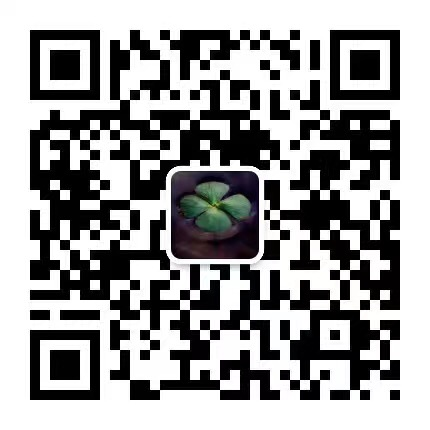
\includegraphics[scale=0.6]{example/gzh.jpg}}
\centerline{\fontsize{26pt}{26pt} 微信公众号}
\end{pre}
\pagestyle{empty}
\tableofcontents
\cleardoublepage
%# -*- coding: utf-8-unix -*-
\begin{overview}
\thispagestyle{empty}
在2018年3月底,翻译\footnote{这个模板原本是用于一项书籍翻译计划的,关注我公众号的读者对此有所了解。然而由于版权原因,该译本无法公开分享。}进度已过大半,于是开始着手进行\LaTeX 排版。在此之前我对\LaTeX 的了解微乎其微,甚至第一次安装TexLive就出了问题,不得不重新安装。也是借着给这个译本排版的机会,才逐渐熟悉了这一软件的使用方法。

如大家所见,模板的封面和扉页设计均高仿\footnote{李老师的书籍源码尚未公开,此为仿作。}自李文威老师《模形式初步》一书,并已得到李老师的使用许可;定理和定义环境则取材自网上流传的Elegantbook模版。我也从这一以模仿为主的学习过程中,对\LaTeX 有了更深入的了解。

本模板命名为$\mathbb{ Q }$-book,谐音自cubic一词。由于是一个菜鸟的作品,自然还有许多瑕疵,对此模板的错误和不足之处还请各位多多包涵。

\end{overview}

\mainmatter	  % 对正文用阿拉伯数字作为页码
%======================================================================
% 正文内容
\pagestyle{fancy}
\setcounter{page}{0}
%# -*- coding: utf-8-unix -*-
%%==================================================
\chapter{多任务联合学习}

\section{Multi-Task Learning Using Uncertainty to Weigh Losses for Scene Geometry and Semantics}

论文地址: \href{https://arxiv.org/abs/1705.07115v3}{Multi-Task Learning Using Uncertainty to Weigh Losses for Scene Geometry and Semantics}

参考资料: \href{https://zhuanlan.zhihu.com/p/65137250}{多任务损失优化1},\href{https://blog.csdn.net/cdknight_happy/article/details/102618883}{多任务损失优化2},\href{https://blog.csdn.net/qq_41214679/article/details/110750812}{多任务损失优化3}

\subsection{问题提出}

\subsubsection{多任务学习介绍}

以前多任务的总损失函数可用如下表达式表示
\begin{align}
& L_{total} = \sum_i w_iL_i
\end{align}

只是简单的对每个子任务进行线性求和,这样会存在很多问题,例如模型对于权重参数很敏感,如下图\href{fig:1-1}{1-1}所示
\begin{figure}
  \centering
  % Requires \usepackage{graphicx}
  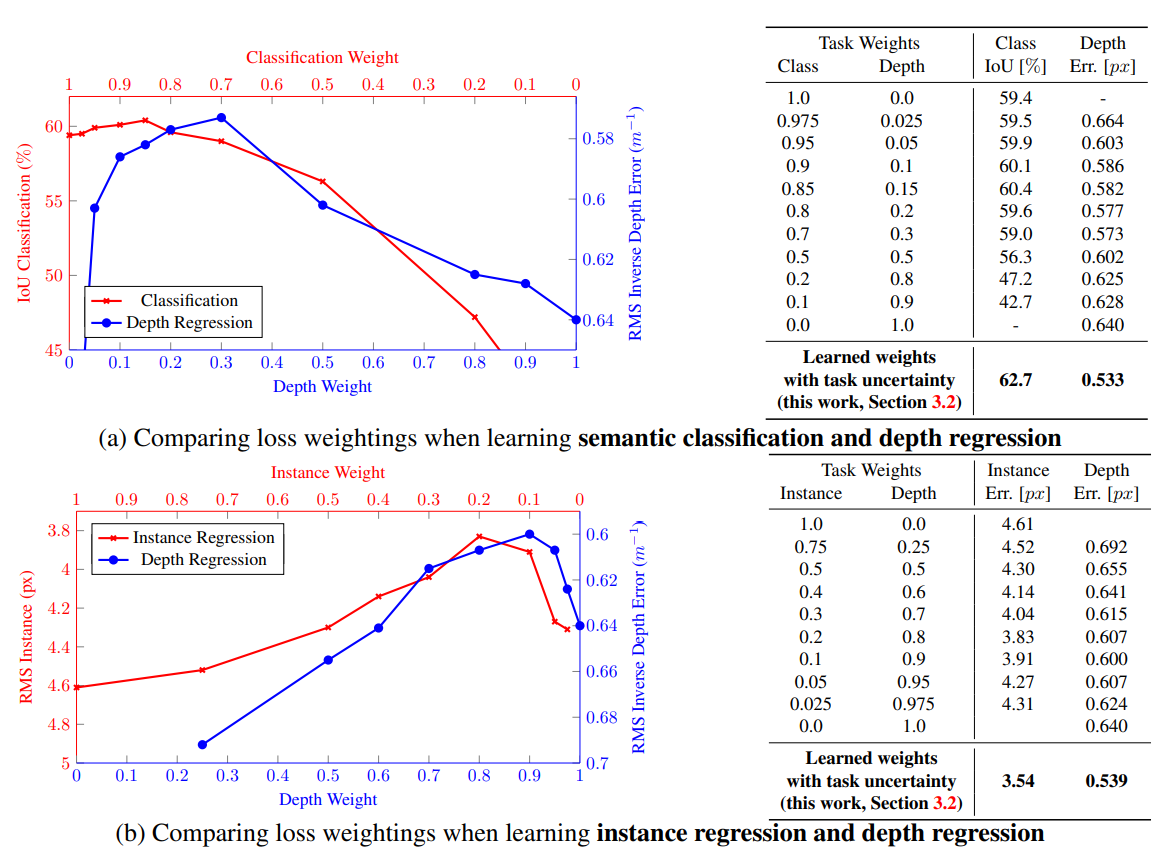
\includegraphics[width=4.5in]{figure/example/2.png}\\
  \caption{不同任务对权重参数很敏感}
  \label{fig:1-1}
\end{figure}

\subsubsection{本文创新点}

多任务联合学习可以提升各任务的学习效果,因为多任务可以共享数据集、共享低层特征。但多任务联合学习时,该如何对各子任务的损失函数进行加权才能取得最优的训练效果,这是本文所关心的问题。

本文中作者提出的多任务如下图\href{fig:1-2}{1-2}所示:
\begin{figure}
  \centering
  % Requires \usepackage{graphicx}
  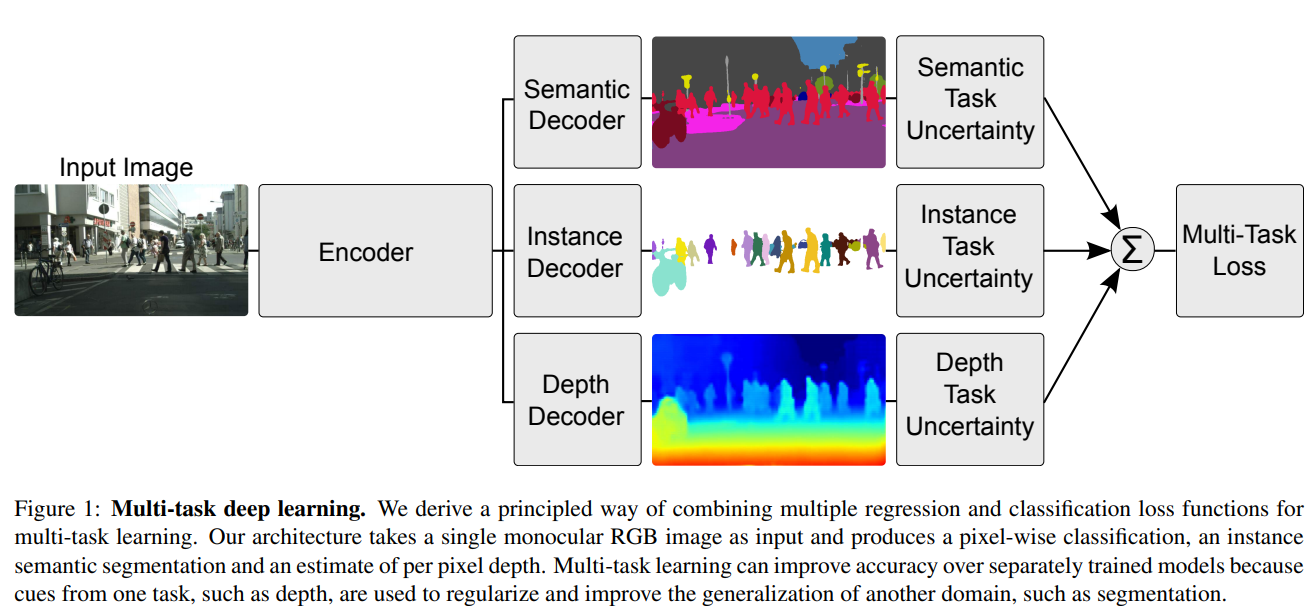
\includegraphics[width=5.5in]{figure/example/1.png}\\
  \caption{论文中用到的多任务图}
  \label{fig:1-2}
\end{figure}

本论文创新点:
\begin{enumerate}
    \item 利用同方差不确定性同时学习不同数量和单元的分类和回归损失的一种新颖多任务损失
    \item 建立统一的组合语义分割、定位分割和深度回归体系结构
    \item 证明模型损失权重的重要性,并且能够解决并获得良好的参数。
\end{enumerate}

\subsection{解决方案}

\subsubsection{多任务似然}
下面通过最大化同方差不确定性的最大高斯似然估计来推导多任务损失函数。

假设输入数据为X,参数矩阵为W,模型输出为$f^W(x)$,真实输出为$y$,这里的$f^W(x)$可以理解成多个子任务的输出汇总。

1、对于回归任务,定义其概率是以输出为均值的高斯似然,即
\begin{align}
& p(y|f^W(x)) = N(f^W(x),\sigma^2)
\end{align}
这个函数可以理解成:真实输出$y$和输出值$f^W(x)$之间(也就是误差)服从正态分布,标准差为$\sigma$

2、对于分类任务,通过Softmax将输出转化为概率,即:
\begin{align}
& p(y|f^W(x)) = Softmax(f^W(x))
\end{align}

3、对于多任务模型(输出是相互独立的),其似然为:
\begin{align}
& p(y_1,...,y_k|f^W(x)) = p(y_1|f^W(x))...p(y_K|f^W(x))
\end{align}

其中

正态分布的概率密度函数为
\begin{align}
& f(x) = \frac{1}{\sqrt{2 \pi}\sigma}exp(-\frac{(x - \mu)^2}{2\sigma^2})
\end{align}

Softmax表达式为
\begin{align}
& softmax(X)_{ij} = \frac{exp(X_{ij})}{\sum_k exp(X_{ik})}
\end{align}

\subsubsection{回归任务}

对于回归任务,即公式(2),其对数似然为:
\begin{align}
&\log p(y|f^W(x)) \propto - \frac{1}{2\sigma^2}||y - f^W(x)||^2 - log \sigma
\end{align}

其中,$\sigma$是高斯似然的标准差,也是模型的噪声参数,表示输出数据中的噪声量。我们的目的是基于参数矩阵$W$和标准差$\sigma$最大化对数似然。

假设多任务模型进行两个回归任务,两个任务都符合高斯分布,输出分别是 $y_1$和$y_2$,那么总的对数似然为:
\begin{align}
&p(y_1,y_2 | f^W(x)) = p(y_1|f^W(x))p(y_2|f^W(x)) \nonumber \\
&= N(y_1;f^W(x),\sigma^2_1)N(y_2;f^W(x),\sigma^2_2)
\end{align}

取对数,优化目标变成了最大化对数似然,也是最小化负对数似然,即:
\begin{align}
& = -\log p(y_1,y_2 | f^W(x)) \nonumber \\
&\propto \frac{1}{2\sigma^2_1}||y_1 - f^W(x)||^2 + \frac{1}{2\sigma^2_2}||y_2 - f^W(x)||^2 + \log \sigma_1 \sigma_2 \nonumber \\
& = \frac{1}{2\sigma^2_1}L_1(w) + \frac{1}{2\sigma^2_2}L_2(w) + \log \sigma_1 \sigma_2
\end{align}

要是想最小化负对数似然,就需要调整$\sigma_1$ 和 $\sigma_2$的值。 $\sigma_1$ 增加,$L_1(w)$会减小,反之亦然。最后项影响不大,可以当作正则化项。

\subsubsection{分类任务}

对于分类任务的概率,添加一个标量缩放系数$\sigma^2$
\begin{align}
&p(y|f^W(x),\sigma) = Softmax(\frac{1}{\sigma^2}f^W(x))
\end{align}

这被称作是Boltzmann分布,也叫做吉布斯分布。系数$\sigma^2$可以是设定的,也可以是通过学习得到的,决定离散分布的平坦程度。该值和分布的不确定性(熵)有关。其对数似然可以写成:
\begin{align}
log(y=c|f^W(x),\sigma) = \frac{1}{\sigma^2}f_c^W(x) - log(\sum_{c'}exp(\frac{1}{\sigma^2}f^W_{c'}(x)))
\end{align}

\subsubsection{回归和分类任务}
假设一个多任务模型由一个分类任务和一个回归任务组成,那么联合损失为:
\begin{align}
& -\log p(y_1,y_2 = c|f^W(x)) \nonumber \\
& = - \log N(y_1;f^W(x),\sigma_1^2) \cdot Softmax(y_2 = c;f^W(x),\sigma_2) \nonumber \\
& = \frac{1}{2\sigma^2_1}||y_1 - f^W(x)||^2 + log\sigma_1 - \log p(y_2 = c | f^W(x),\sigma_2) \nonumber \\
& = \frac{1}{2\sigma^2_1}L_1(W) +\frac{1}{\sigma^2_2}L_2(W)+ \log \sigma_1+ \log\frac{\sum_{c'}exp(\frac{1}{\sigma^2_2}f_{c'}^W(x))}{(\sum_{c'}exp(f_{c'}^W(x))^{\frac{1}{\sigma^2_2}}}\nonumber \\
&\approx \frac{1}{2\sigma_1^2}L_1(W) + \frac{1}{\sigma^2_2}L_2(W)+\log\sigma_1+ \log\sigma_2
\end{align}

上式中,$L_1(W) = || y_1-f^W(x)||^2$,为回归子任务输出和真实label = $y_1$ 间的欧式距离。 $L_2(W)=-\log (Softmax( y_2 , f^W(x)))$是分类子任务的交叉熵损失。对于最后一项,我们假设是约等的,即
\begin{align}
& \frac{1}{\sigma_2}\sum_{c'}exp(\frac{1}{\sigma^2_2}f_{c'}^W(x)) \approx (\sum_{c'}exp(f_{c'}^W(x))^{\frac{1}{\sigma^2_2}}
\end{align}

当$\sigma_2 = 1$时,上式等号成立。优化的目的是同时寻找最优的$W$、$\sigma_1$和$\sigma_2$。

最终的目标可以看成是学习每一个子任务输出的相对权重。大的$\sigma_2$会降低$L_2(W)$的影响,小的$\sigma_2$会增大$L_2(W)$的影响。

作者最终的做法是在模型训练的过程中去优化$\sigma_1$和$\sigma_2$,并且为了提升数值稳定性,作者去学习参数$s:=\log \sigma^2$。


\subsection{实验结果}

实验结果如图\href{fig:1-3}{1-3}所示, 得出的结论是基于三个任务的不确定性进行损失加权的效果最好。
\begin{figure}
  \centering
  % Requires \usepackage{graphicx}
  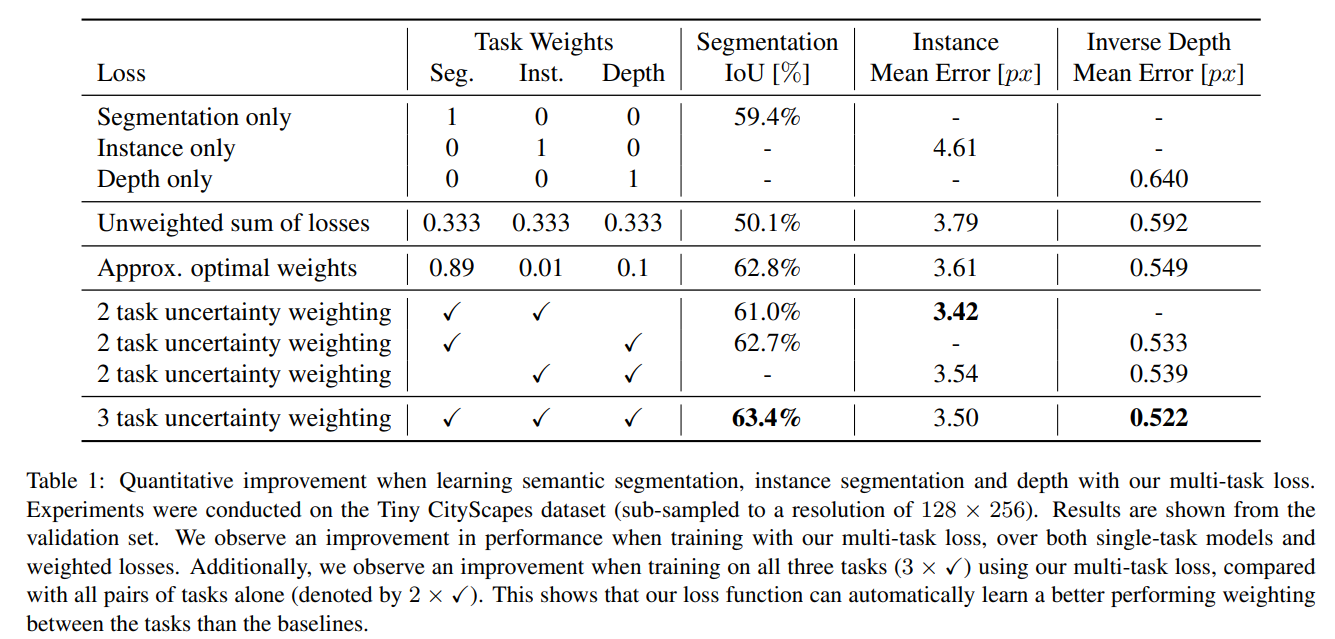
\includegraphics[width=5in]{figure/example/3.png}\\
  \caption{实验结果图}
  \label{fig:1-3}
\end{figure}

\subsection{参考代码}

多任务联合学习的特点是不同子任务共享低层特征,并通过不同子任务的协同学习进行信息的交互,在相互促进中完成整个任务。举个计算机视觉的例子,在计算机视觉感知上,任务级别从低到高可以划分为:物体分类,目标检测,语义分割和实例分割。如果想通过端到端方式训练整个模型,完成所有任务,我们必须为这些任务分配合理的权重。假设目标检测和语义分割可以实现端到端学习的话,那么如果目标检测在训练上表现的效果很差,语义分割的效果也不会好到哪去。我们在训练模型完成多个任务时,期待这些相互协同的任务是往相互促进的方向发展,而不是相互制约。

在作者给出的参考代码中,以两个回归任务联合学习为例,其对应的联合损失如下:

\begin{align}
& = -\log p(y_1,y_2 | f^W(x)) \nonumber \\
&\propto \frac{1}{2\sigma^2_1}||y_1 - f^W(x)||^2 + \frac{1}{2\sigma^2_2}||y_2 - f^W(x)||^2 + \log \sigma_1 \sigma_2 \nonumber \\
& = \frac{1}{2\sigma^2_1}L_1(w) + \frac{1}{2\sigma^2_2}L_2(w) + \log \sigma_1 \sigma_2
\end{align}

假设我们手头上有服从正态分布的,样本数为1024一维随机样本$X$,通过这些样本,我们分别添加了方差为10,方差为1的线性随机噪声$y1$,$y2$,如图\href{fig:1-4}{1-4}所示。
\begin{figure}
  \centering
  % Requires \usepackage{graphicx}
  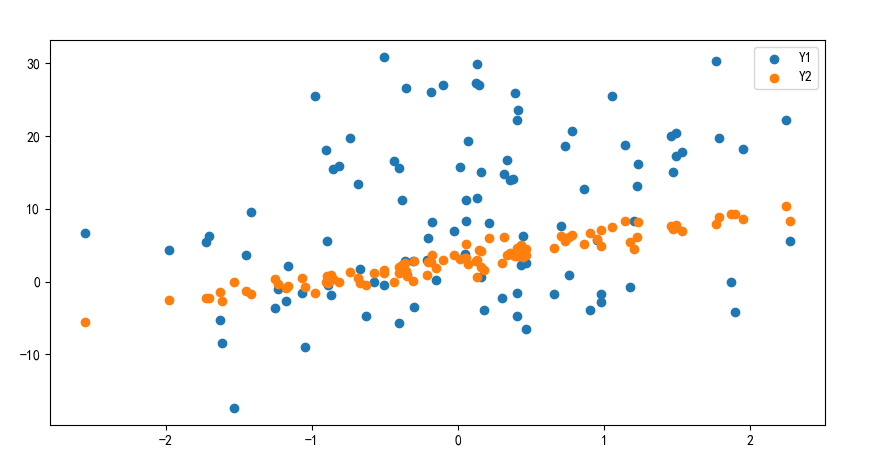
\includegraphics[width=5in]{figure/example/4.png}\\
  \caption{方差为10,方差为1的线性随机噪声y1,y2}
  \label{fig:1-4}
\end{figure}

\begin{lstlisting}[language={C}, caption={数据生成代码}]
 '''Evaluate on synthetic data'''
N = 100
nb_epoch = 2000
batch_size = 20
nb_features = 1024
Q = 1
D1 = 1  # first output
D2 = 1  # second output

def gen_data(N):
    X = np.random.randn(N, Q)
    w1 = 2.
    b1 = 8.
    sigma1 = 1e1  # ground truth 方差为10
    Y1 = X.dot(w1) + b1 + sigma1 * np.random.randn(N, D1)  #添加方差为10的线性随机噪声
    w2 = 3.
    b2 = 3.
    sigma2 = 1e0  # ground truth 方差为1
    Y2 = X.dot(w2) + b2 + sigma2 * np.random.randn(N, D2)  #添加方差为1的线性随机噪声
    return X, Y1, Y2
\end{lstlisting}

接着我们定义一个简单的模型来同时拟合这两组数据。因为输入的样本维数只有1维,因此我们定义一个神经元作为输入层,接着定义一个含1024个神经元的全连接层,并在每个单元后连接一个Relu非线性激活函数,进行特征提取。整个全连接层可以对一个样本提取1024维的特征。

接着我们定义两个神经元作为输出层,这两个神经元分别代表两个子任务,这两个子任务共享前面隐藏层提取的特征,并分别对方差为10,方差为1的线性随机噪声进行拟合。

接下来就是本文的重点了:我们根据式子\href{1-14}{1-14},定义一个MultiLoss层,并将输出层中两个神经元作为输入,核心代码如下所示。

\begin{lstlisting}[language={C}, caption={MultiLoss Layer核心代码}]
 def multi_loss(self, ys_true, ys_pred):
        assert len(ys_true) == self.nb_outputs and len(ys_pred) == self.nb_outputs
        loss = 0
        #这里以两个回归任务为例
        for y_true, y_pred, log_var in zip(ys_true, ys_pred, self.log_vars):
            precision = (K.exp(-log_var[0]))
            loss += K.sum(precision * (y_true - y_pred) ** 2. + log_var[0], -1)

        return K.mean(loss)
\end{lstlisting}

最后输出结果为$[\frac{1}{\sigma_1^2} = 8.648183872325495, \frac{1}{\sigma_2^2} = 0.9251061404392964]$,分别对应在方差为10,方差为1线性随机噪声下损失函数的权值。我们可以发现,线性随机噪声的方差越大,信息的不确定性越大,子任务的损失函数被赋予的权值也就越大。整个模型如图\href{fig:1-5}{1-5} 所示。

\begin{figure}
  \centering
  % Requires \usepackage{graphicx}
  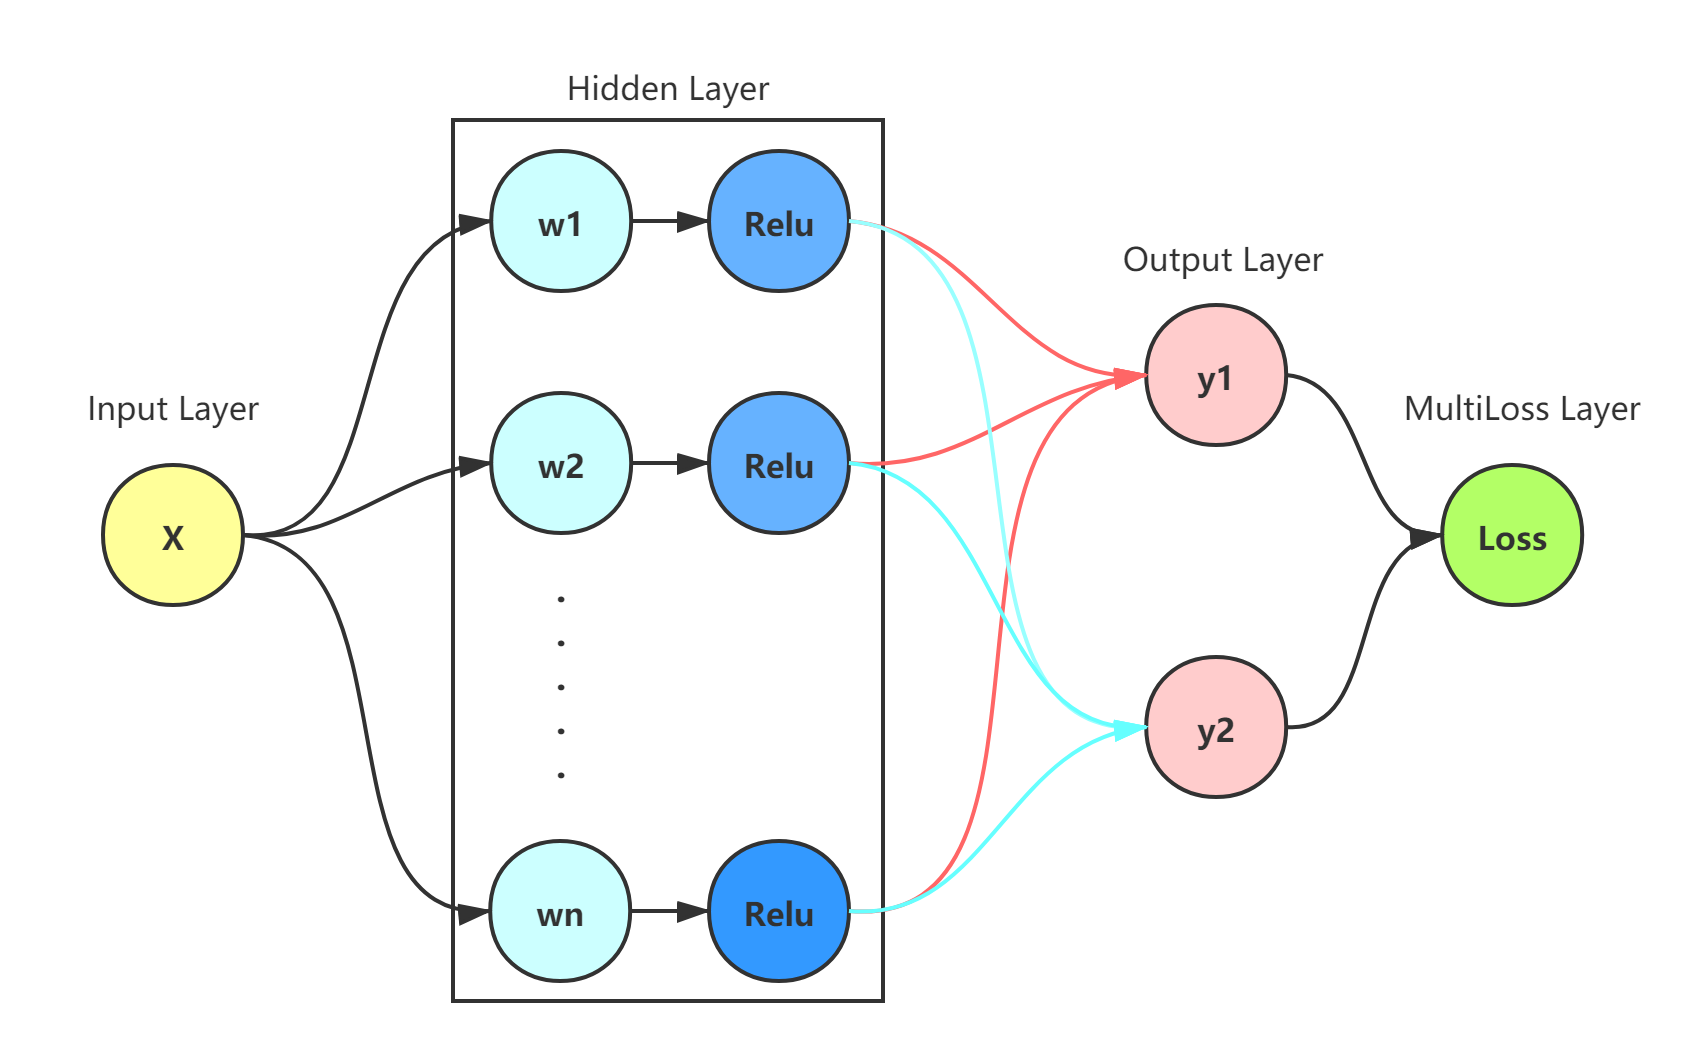
\includegraphics[width=5in]{figure/example/MultiLoss.png}\\
  \caption{多任务损失模型图}
  \label{fig:1-4}
\end{figure}

\subsection{小总结}

作者利用参考代码中简单的小例子,提出了一种多任务联合损失函数优化的方法(上面大部分小节都在讲这个损失函数的推导过程),并尝试将其应用在语义分割,实例分割,深度回归三个子任务所构成的总任务中,发现基于三个子任务的同方差不确定性损失加权效果最好。

一般来说,对于单任务输出的损失函数值是一个标量,而多任务的损失函数输出值是一个向量。如果损失函数值是一个向量的话,则需要通过线性求和来计算总的损失,即$L_{total}    = \sum_i w_i L_i$。在本文中,作者在基于回归任务的输出服从高斯分布,分类任务的输出服从玻尔兹曼分布的假设下,通过高斯似然和Softmax函数,定义了一个多任务联合损失函数(对数似然函数),通过最小化损失函数(最大似然估计)来确定这两个任务的参数,而非简单的线性加权求解参数。

整个任务的总体损失受不同重要因子的子任务共同影响。这个重要因子由输出数据的方差来决定,方差越大,信息不确定性越大,loss被赋予的权重也越大,进而应优先学习不确定性更大的子任务,使整个任务在全局输出上达到最优。

\subsection{补充知识}

\subsubsection{同方差不确定性}

在介绍相关知识前,先简单了解一下什么是"不确定性”。在很多情况下,深度学习领域都有极佳的表现,这种表现依赖于大量的数据,强大的算力,深厚的网络结构,会对某一个问题给出一个特定的答案,这个答案是给定模型在众多候选中找到概率最大的(比如分类问题最后用softmax)得到的,但是在极端情况下,答案的唯一输出会存在些问题。

如果训练的类别只包含A类和B类,但在测试阶段输入C 类的图片,那么分类器大概率会将自己所学到的类别作为输出结果,而这种错误,在容错率极低的行业,如航天,军事等领域,是绝不能容忍的。试想一下,如果面对这种极端情况,在输出结果的同时给出一个极低的相对于结果的置信度,这个低置信度会带来预警,让人为进行干预,效果会更好。这种置信度的输出,就要靠贝叶斯建模了。\\

在贝叶斯建模中,需要解决两种不同类型的不确定性。
\begin{enumerate}
    \item 认知不确定性:表示的是模型本身的不确定性,这是因为缺乏训练数据,模型认知不足,可以通过扩充训练集进行解决;
    \item 偶然不确定性:偶然不确定性表示数据不能解释的信息。举一个例子,在数据标注时如果出现比较大的标注误差,这个误差不是模型带入的,而是数据本身就存在的,数据集里的bias越大,偶然不确定性就越大。这也是贝叶斯派引入先验概率来修正原有数据在统计中产生误差的原因。
\end{enumerate}

偶然不确定性又分成两类:
\begin{enumerate}
    \item 数据依赖型或异方差不确定性(Data-dependent or Heteroscedastic uncertainty):这种不确定性取决于输入的数据,并且预测结果作为模型的输出。
    \item 任务依赖型或同方差不确定性(Task-dependent or Homoscedastic uncertainty):不取决于输入数据,而是取决于不同的任务。对于所有的输入数据,它们具有相同的常量,而对于不同的任务,它们有不同的变量。基于这个特性,我们称之为任务依赖型不确定性。
\end{enumerate}

因为在多任务学习中,任务的不确定性表明了任务间的相对置信度,反映了回归和分类问题中固有的不确定性。因此本文提出把同方差不确定性作为噪声来对多任务学习中的权重进行优化。\\

为了更好地理解后面提到的参考代码,这里先理解一下同方差的2个基本假设:
\begin{enumerate}
    \item 假设一被称为(White Noise Condition)白噪音假设,干扰项即误差部分相互没有关联。假设回归式$y=\alpha + \beta x + u$, 其误差项中,$u1,u2$各误差之间没有任何联系,即:协方差矩阵$COV(u1 * u2)= 0$。
    \item 假设二为干扰项具备同方差性或者等分散, 即误差项与独立变量(independent variable)之间相互独立, 并且误差项的分散(方差)必须等同,即$Var(u|x)=\sigma^2$;解释变量之间不存在多重共线性;解释变量是确定变量。
\end{enumerate}

\subsubsection{频率派和贝叶斯派}

在概率估计或者机器学习里的参数估计上,有两个方法,MLE(最大似然估计) 和MAP(最大后验估计),其实代表了概率论里的两个派别,频率派和贝叶斯派\footnote{频率派vs贝叶斯派 \quad \url{https://blog.csdn.net/weixin_43593330/article/details/105797717}}。 在了解这两个派别所研究内容有啥区别之前,我们有必要先理清一些基础概念:什么是似然函数,什么是概率函数,什么是MLE,MAP。\\

1、似然函数 和 MLE(最大似然估计)

在统计学中,假设我们对含未知参数的模型给定一个参数值,似然函数可以用来衡量这个模型对于数据样本的拟合程度。似然函数由样本的联合概率分布构成,并作为关于参数的函数。通过似然函数最大化来求解这些参数,即最大似然估计。为了计算方便,通常使用对数似然函数。在概率论的两个派别中,似然函数都起着基础性的作用。\\

在MLE中,首先要定义似然函数$$
\begin{align}
& L(\theta|x) = f_D(x_1,x_2,...,x_n|\theta) \nonumber \\
& = \prod_{i = 1}^n p(x_i;\theta)
\end{align}

在$\theta$的所有取值上,使这个函数最大化,这个使可能性最大的值即为MLE(一般求解步骤见Wiki)。

这里举个例子:假设有一个造币厂生产某种硬币,现在我们拿到了一枚硬币,想试试这硬币是不是均匀的,我们可以通过抛硬币的方式,统计硬币正反面出现的概率(记为$\theta$),如果正反面出现的概率相同,则该硬币是均匀的,反之亦然\footnote{贝叶斯公式理解与应用 \quad \url{https://blog.csdn.net/qq_33934427/article/details/105002894}}。

于是我们拿这枚硬币抛了10次,得到的数据($x_0$)是:"反正正正正反正正正反",其中正面概率$\theta$是我们想求的模型参数,我们可以得到似然函数
\begin{align}
& f(x_0,\theta)=(1-\theta) \times \theta \times \theta \times \theta \times \theta \times (1-\theta) \times \theta \times \theta \times \theta \times (1-\theta)=\theta^7(1-\theta)^3 = f(\theta)
\end{align}

实验得到的似然函数值为0.7,这能说明该厂生产的硬币是不均匀吗?显然是不行的,实验的次数太少了,如果实验次数达到上千次,正负面统计的频数或许各占一半。\\

2、MAP(最大后验估计)

最大似然估计通过求解参数$\theta$, 使似然函数$P(x0|\theta)$最大。而最大后验概率估计则是在求解$\theta$过程中,使$P(x0|\theta)P(\theta)$最大。要想使后验概率尽可能大,关于$\theta$的似然函数要大,$\theta$自己出现的先验概率也要大。这有点像正则化里加惩罚项的思想,不过正则化里是利用加法,而MAP里是利用乘法。MAP公式如下

\begin{align}
& P(\theta|x0)=\frac{P(x0|\theta)P(\theta)}{P(x0)}
\end{align}

由于MAP在计算过程中,$x0$是确定的。如果还是拿上面MLE的例子,$x0$ 表示硬币投出正反面数:“反正正正正反正正正反”,假设“投10次硬币”是一次实验,实验做了1000 次,“反正正正正反正正正反”出现了n次,则$P(x0)=n/1000$。因此$P(x0)$是一个已知值,所以在计算MAP时可以去掉分母$P(x0)$

MAP在最大化$P(\theta|x0)$ 的意义也很明确,$x0$已经确定了,求$\theta$ 使$P(\theta|x0)$ 最大。\\

3、概率函数和似然函数

对于如下函数,假设输入有两个:$x$表示某一个具体的数据; $\theta$ 表示模型的参数。
\begin{align}
& P(x|\theta)
\end{align}

若$\theta$是已知确定的,$x$是变量,这个函数叫做概率函数,它描述在给定模型参数$\theta$,对于不同的样本点$x$其出现概率是多少(softmax)。最大后验概率估计目的是求$x$,即
\begin{align}
& p(X|\theta) = \max\{p(x_1 | \theta),p( x_2 | \theta), ... , p( x_3 | \theta)\}
\end{align}

如果$x$是已知确定的,$\theta$是变量,这个函数叫做似然函数,它描述对于不同的模型参数,出现$x$这个样本点的概率是多少。最大似然估计目的是求参数$\theta$,即
\begin{align}
& p(X|\theta) = \max\{p(X | \theta_1),p( X | \theta_2), ... , p( X | \theta_n)\}
\end{align}

\quad

4、统计和概率的区别:

概率(probabilty)和统计(statistics)看似两个相近的概念,其实研究的问题刚好相反。
\begin{itemize}
    \item 概率研究的问题是,已知一个模型和参数,怎么去预测这个模型产生的结果的特性(例如均值,方差,协方差等等)
    \item 统计研究的问题是,有一堆数据,要利用这堆数据去预测模型和参数。
\end{itemize}

一句话总结:概率是已知模型和参数,推数据。统计是已知数据,推模型和参数。\\

5、小总结

往大的说,这两个派别代表了不同的世界观。频率派认为参数($\theta$) 是客观存在不会改变的,虽然未知,但却是固定值。贝叶斯派则认为参数是随机值,因为不可能做完整的实验去确定,因此参数也可以有分布。

往小处说,频率派最常关心的是似然函数,他们认为直接用样本去计算出的概率就是真实的,而贝叶斯派最常关心的是后验分布,他们认为样本只是用来修正经验观点。

贝叶斯派因为所有的参数都是随机变量,都有分布,因此可以使用一些基于采样的方法 (如MCMC)使得我们更容易构建复杂模型。频率派的优点则是没有假设一个先验分布,因此更加客观,也更加无偏,在一些保守的领域(比如制药业、法律)比贝叶斯方法更受到信任。

本质上MLE是根据样本数据直接计算概率参数,而MAP是预设一个参数的概率分布,然后通过样本数据去进行修正。如果样本量不够大的时候,MAP 可能更符合人们的日常经验,比如一个硬币抛五次,都是正面朝上,那么MLE算出来就是这个硬币正面朝上概率为100$\%$,而用先验概率50$\%$加上MAP去算,可能只是51$\%$,更符合人们的日常经验。

如果样本量足够大,这两个方法还是殊途同归的,都是进行参数估计。如果样本量适中,那么MAP使用比较合理的先验概率是很重要的。 \\

6、谈谈我的理解

最大似然估计和最大后验概率,它们两者目的一致,都是为了进行参数估计。频率派认为数据样本是客观可靠的,相信从中统计样本可以进行参数估计,因此最大似然估计则是在给定样本中计算最大的联合概率,求解这个参数,该参数模型对数据样本拟合最好。

而贝叶斯派认为数据样本不可靠,单纯通过对数据样本的统计可能会存在问题,因此最大后验概率需要先给定某个参数的先验概率(这个先验概率可以通过专家讨论得到)作为”正则化项”,来修正通过数据样本计算似然函数时存在的不准确的问题

核心思想搞懂了,再来看看MLE,MAP在计算中,谁是已知的,谁是未知的,这样才不容易搞混:MLE中参数未知,x已知(因为对数据样本统计求解参数),MAP中参数已知(有先验概率),x未知(x不可靠,需要利用先验概率来修正似然函数),最终目的都是为了求解最优参数(参数是个广泛的概念,比如硬币的正反面,单词的含义等)。



%# -*- coding: utf-8-unix -*-
%%==================================================

\chapter{写作示例}
\label{chap2}

\section{列表环境}

\subsection{无序列表}

以下是一个无序列表的例子,列表的每个条目单独分段。

\begin{itemize}
	\item 这是一个无序列表。
	\item 这是一个无序列表。
	\item 这是一个无序列表。
\end{itemize}

使用\verb+itemize*+环境可以创建行内无序列表。
\begin{itemize*}
	\item 这是一个无序列表
	\item 这是一个无序列表
	\item 这是一个无序列表
\end{itemize*}
行内无序列表条目不单独分段,所有内容直接插入在原文的段落中。

\subsection{有序列表}

使用环境\verb+enumerate+和\verb+enumerate*+创建有序列表,
使用方法无序列表类似。
\begin{enumerate}
	\item 这是一个有序列表。
	\item 这是一个有序列表。
	\item 这是一个有序列表。
\end{enumerate}

使用\verb+enumerate*+环境可以创建行内有序列表。
\begin{enumerate*}
	\item 这是一个默认有序列表
	\item 这是一个默认有序列表
	\item 这是一个默认有序列表
\end{enumerate*}
行内有序列表条目不单独分段,所有内容直接插入在原文的段落中。

\subsection{描述列表}
使用环境\verb+description+可创建带有主题词的列表,条目语法是\verb+\item[主题] 内容+。
\begin{description}
	\item[主题一] 详细内容
	\item[主题二] 详细内容
	\item[主题三] 详细内容 \ldots
\end{description}

\section{数学排版}

\subsection{公式排版}

这里有举一个长公式排版的例子,来自\href{http://www.tex.ac.uk/tex-archive/info/math/voss/mathmode/Mathmode.pdf}{《Math mode》}:

\begin {multline}
\frac {1}{2}\Delta (f_{ij}f^{ij})=
2\left (\sum _{i<j}\chi _{ij}(\sigma _{i}-
\sigma _{j}) ^{2}+ f^{ij}\nabla _{j}\nabla _{i}(\Delta f)+\right .\\
\left .+\nabla _{k}f_{ij}\nabla ^{k}f^{ij}+
f^{ij}f^{k}\left [2\nabla _{i}R_{jk}-
\nabla _{k}R_{ij}\right ]\vphantom {\sum _{i<j}}\right )
\end{multline}

\subsection{SI单位}

使用\verb+siunitx+宏包可以方便地输入SI单位制单位,例如\verb+\SI{5}{\um}+可以得到\SI{5}{\um}。

\subsection{定理环境}

在这个模板中,定义了如下几个环境
remark(注),mythm(定理),myprop(性质),mydef(定义),example(例)。
amsmath还提供了一个proof(证明)的环境。
我们举例说明它们的用法。

注环境
\begin{remark}
	存在事先给定的一系列基本操作,并且这些基本操作永远不会改变。
\end{remark}
\begin{remark}
	每个操作都可逆。
	\label{o1.2}
\end{remark}
\begin{remark}
	每一个操作都是确定性的。
\end{remark}
\begin{remark}
	各个操作可以按任何顺序组合。
\end{remark}

性质环境
\begin{myprop}{}{}
	存在一些预先定义的永不发生改变的作用(action)。
\end{myprop}

\begin{myprop}{}{}
	每一个作用都可逆。
\end{myprop}

\begin{myprop}{}{}
	每个作用都是确定性的。
\end{myprop}

\begin{myprop}{}{}
	任意的一系列连续的作用仍然是一个作用。
\end{myprop}

例子环境
\begin{example}
	天地玄黄,宇宙洪荒。
	\soln
	
	日月盈仄,辰宿列张。
\end{example}

定义环境
\begin{mydef}{域}{1}
	设$S$为一个非空集合,其上有“加法”(记作$+$)与“乘法”(记作$\cdot$)两种代数运算. 若满足以下条件,则称$(S,+,\cdot)$构成一个域(field).
	\begin{itemize}
		\item[(1)] $(S,+)$构成一个交换群.
		\item[(2)] 若记$S^{*}=S-\{0\}$,其中$0$为群$(S,+)$中的单位元,则$(S^{*},\cdot)$也构成一个交换群.
		\item[(3)] 乘法对加法有分配律:$a ( b + c ) = a b + a c$.
	\end{itemize}
\end{mydef}

关键点环境
\begin{keypoint}
	伽罗瓦理论在分析从有理数域$\mathbb{ Q }$扩张到新的域的运算或操作时很有用。我们的大问题可以用伽罗瓦理论来回答,数学中其他的一些历史问题也同样可以用伽罗瓦理论来解答。
\end{keypoint}

定理环境
\begin{mythm}{望远镜公式}{2}
	$\left[\mathbb{Q}(a, b) : \mathbb{Q}\right]=\left[\mathbb{Q}(a, b) : \mathbb{Q}(a)\right]\left[\mathbb{Q}(a) : \mathbb{Q}\right] $
\end{mythm}

\begin{proof}
	
	\rthm{thm:2}告诉我们,对任意$s\in S$,均有$\lvert Orb(s)\rvert \cdot \lvert Stab(s)\rvert=\lvert G\rvert=p$. 于是$\lvert Orb(s)\rvert $整除$p$,这里$p$是一个素数。从而$\lvert Orb(s)\rvert $等于1或$p$,也就是说,\textbf{所有轨道的大小要么为1,要么为$p$}. 于是整个集合$S$就被划分为两部分,一部分是大小为1的轨道,另一部分是大小为$p$的轨道,如图9.4所示。
	
	假设大小为1的轨道有$m$个,大小为$p$的轨道有$n$个,则有
 \begin{equation}
		m+p\cdot n=\lvert S\rvert
 \end{equation}
	注意到\rdef{def:1},\textbf{那些$\lvert Orb(s)\rvert =1$的元素$s$即为稳定元},这就表明有$m$个稳定元。从上式立刻看出$\lvert S \rvert \equiv  m\; (\bmod\; p)$.	
\end{proof}

\section{表格}

这一节给出的是一些表格的例子,如表\ref{tab1}所示。

\begin{table}[!hpb]
	\centering
	\bicaption[指向一个表格的表目录索引]
	{一个颇为标准的三线表格\footnotemark[1]}
	{A Table}
	\label{tab1}
	\begin{tabular}{@{}llr@{}} \toprule
		\multicolumn{2}{c}{Item} \\ \cmidrule(r){1-2}
		Animal & Description & Price (\$)\\ \midrule
		Gnat & per gram & 13.65 \\
		& each & 0.01 \\
		Gnu & stuffed & 92.50 \\
		Emu & stuffed & 33.33 \\
		Armadillo & frozen & 8.99 \\ \bottomrule
	\end{tabular}
\end{table}
\footnotetext[1]{这个例子来自\href{http://www.ctan.org/tex-archive/macros/latex/contrib/booktabs/booktabs.pdf}{《Publication quality tables in LATEX》}(booktabs宏包的文档)。这也是一个在表格中使用脚注的例子,请留意与threeparttable实现的效果有何不同。}

下面一个是一个更复杂的表格,用threeparttable实现带有脚注的表格,如表\ref{tab2}。

\begin{table}[!htpb]
	\bicaption[出现在表目录的标题]
	{一个带有脚注的表格的例子}
	{A Table with footnotes}
	\label{tab2}
	\centering
	\begin{threeparttable}[b]
		\begin{tabular}{ccd{4}cccc}
			\toprule
			\multirow{2}{6mm}{total}&\multicolumn{2}{c}{20\tnote{1}} & \multicolumn{2}{c}{40} &  \multicolumn{2}{c}{60}\\
			\cmidrule(lr){2-3}\cmidrule(lr){4-5}\cmidrule(lr){6-7}
			&www & \multicolumn{1}{c}{k} & www & k & www & k \\ % 使用说明符 d 的列会自动进入数学模式,使用 \multicolumn 对文字表头做特殊处理
			\midrule
			&$\underset{(2.12)}{4.22}$ & 120.0140\tnote{2} & 333.15 & 0.0411 & 444.99 & 0.1387 \\
			&168.6123 & 10.86 & 255.37 & 0.0353 & 376.14 & 0.1058 \\
			&6.761    & 0.007 & 235.37 & 0.0267 & 348.66 & 0.1010 \\
			\bottomrule
		\end{tabular}
		\begin{tablenotes}
			\item [1] the first note.% or \item [a]
			\item [2] the second note.% or \item [b]
		\end{tablenotes}
	\end{threeparttable}
\end{table}

\section{插入图片}

\XeTeX 可以很方便地插入PDF、PNG、JPG格式的图片。插入PNG/JPG的例子如\ref{fig1}所示。
这两个水平并列放置的图共享一个“图标题”(table caption),没有各自的小标题。

\begin{figure}[!htp]
\centering

\includegraphics[width=4cm]{example/by-nc.png}
\hspace{1cm}
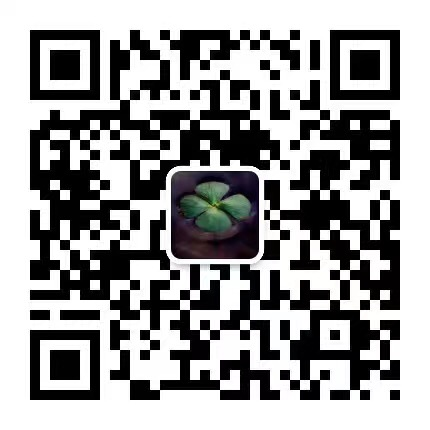
\includegraphics[width=4cm]{example/gzh.jpg}
\bicaption{中文题图}
{English caption}
\label{fig1}
\end{figure}

这里还有插入EPS图像和PDF图像的例子,如图\ref{fig2}和图\ref{fig3}。这里将EPS和PDF图片作为子图插入,每个子图有自己的小标题。子图标题使用subcaption宏包添加。

\begin{figure}[!htp]
\centering
\subcaptionbox{EPS 图像\label{fig2}}[3cm] %标题的长度,超过则会换行,如下一个小图。
{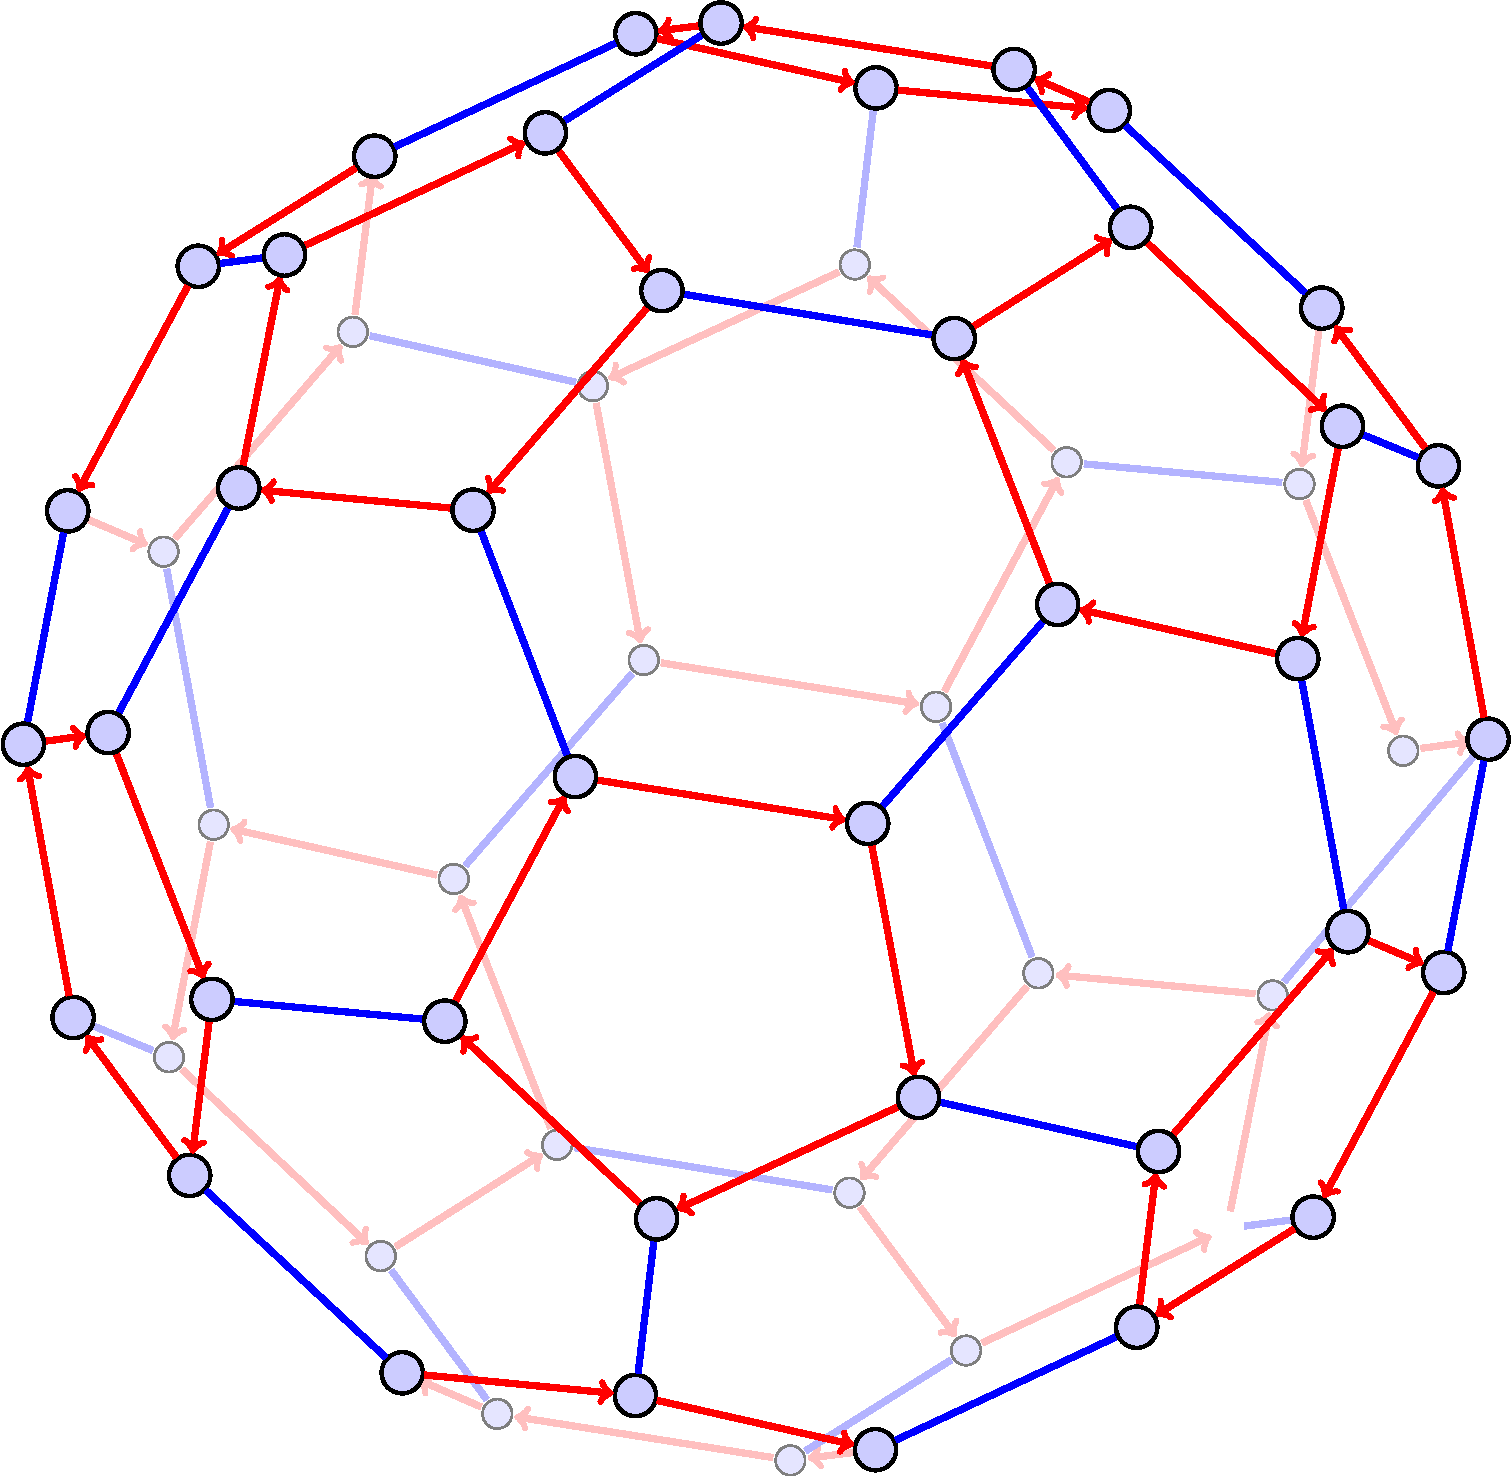
\includegraphics[height=2.5cm]{example/m2.pdf}}
\hspace{4em}
\subcaptionbox{PDF 图像,注意这个图略矮些。如果标题很长的话,它会自动换行\label{fig3}}
{	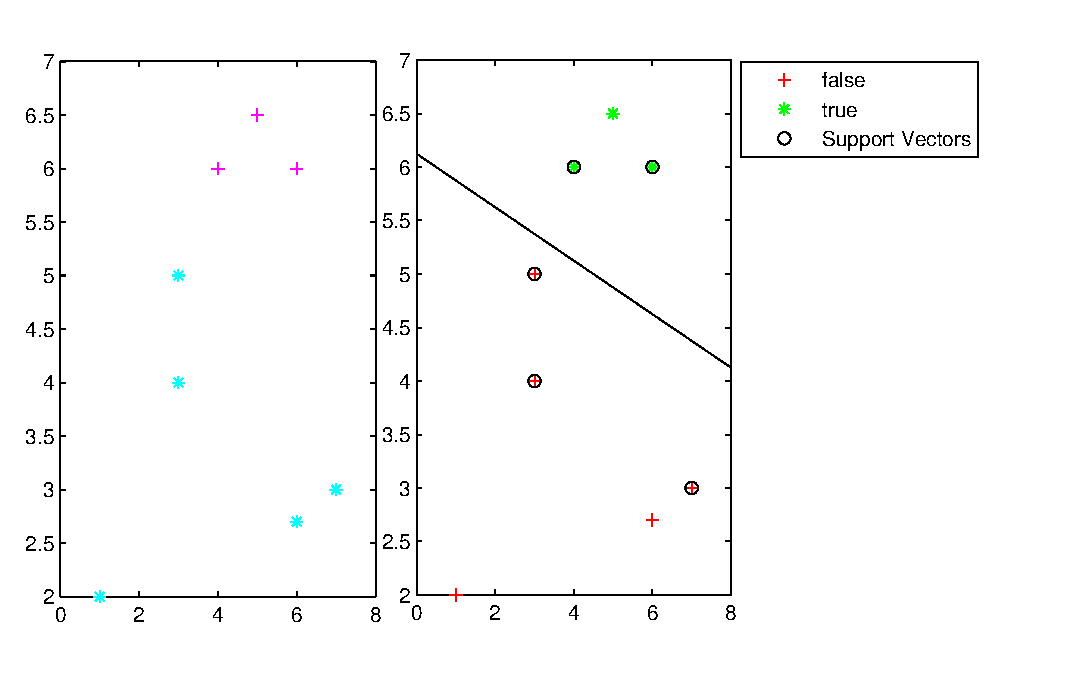
\includegraphics[scale=0.5]{example/figep.eps}}
\bicaption{插入eps和pdf的例子(使用 subcaptionbox 方式)}{An EPS and PDF demo with subcaptionbox}
\label{fig4}
\end{figure}




\section{插入代码}

这里给一个使用listings宏包插入源代码的例子:
\begin{lstlisting}[language={C}, caption={一段C源代码}]
#include <stdio.h>
#include <unistd.h>
#include <sys/types.h>
#include <sys/wait.h>

int main() {
pid_t pid;

switch ((pid = fork())) {
case -1:
printf("fork failed\n");
break;
case 0:
/* child calls exec */
execl("/bin/ls", "ls", "-l", (char*)0);
printf("execl failed\n");
break;
default:
/* parent uses wait to suspend execution until child finishes */
wait((int*)0);
printf("is completed\n");
break;
}

return 0;
}
\end{lstlisting}


\section{参考文献管理}
\label{sec2.5}
\LaTeX 具有将参考文献内容和表现形式分开管理的能力,涉及三个要素:参考文献数据库、参考文献引用格式、在正文中引用参考文献。
这样的流程需要多次编译:
\begin{enumerate}[noitemsep,topsep=0pt,parsep=0pt,partopsep=0pt]
\item 用户将论文中需要引用的参考文献条目,录入纯文本数据库文件(bib文件)。
\item 调用xelatex对论文模板做第一次编译,扫描文中引用的参考文献,生成参考文献入口文件(aux)文件。
\item 调用bibtex,以参考文献格式和入口文件为输入,生成格式化以后的参考文献条目文件(bib)。
\item 再次调用xelatex编译模板,将格式化以后的参考文献条目插入正文。
\end{enumerate}

123456\cite{123a}

参考文献数据库(thesis.bib)的条目,可以从Google Scholar搜索引擎\footnote{\url{https://scholar.google.com}}、CiteSeerX搜索引擎\footnote{\url{http://citeseerx.ist.psu.edu}}中查找,文献管理软件Papers\footnote{\url{http://papersapp.com}}、Mendeley\footnote{\url{http://www.mendeley.com}}、JabRef\footnote{\url{http://jabref.sourceforge.net}}也能够输出条目信息。

下面是在Google Scholar上搜索到的一条文献信息,格式是纯文本:

\begin{lstlisting}[caption={从Google Scholar找到的参考文献条目}, label=googlescholar, escapeinside="", numbers=none]
@phdthesis{"白2008信用风险传染模型和信用衍生品的定价",
title={"信用风险传染模型和信用衍生品的定价"},
author={"白云芬"},
year={2008},
school={"上海交通大学"}
}
\end{lstlisting}

推荐修改后在bib文件中的内容为:

\begin{lstlisting}[caption={修改后的参考文献条目}, label=itemok, escapeinside="", numbers=none]
@phdthesis{bai2008,
title={"信用风险传染模型和信用衍生品的定价"},
author={"白云芬"},
date={2008},
address={"上海"},
school={"上海交通大学"}
}
\end{lstlisting}

参考文献的引用:
\begin{itemize}
\item 参考文献在正文中被引用,使用命令\verb+\cite{key}+,如\cite{M91}。
\item 参考文献未引用但仍希望列在书末的参考文献中,使用命令\verb+\nocite{key}+,如\verb+\nocite{WI64,G03,D01,JS03}+.
\end{itemize}
\nocite{WI64,G03,D01,JS03}

%%# -*- coding: utf-8-unix -*-

\chapter{如何避免"破罐子破摔"的心态 - 网友篇}

破罐子破摔是指:罐子已经破了,又往破里摔。比喻有了缺点、错误或受到挫折以后,任其自流,不加改正,或反而有意朝更坏的方向发展。

\section{网友1 - 停止自责,即使止损}

这种现象特别常见。一种是:吃了一口薯片,然后对自己说再吃一片把,然后一片又一片,一不小心一包薯片没了,心里想完蛋了,之前白克制了,心情很不好,心想反正已经吃了,那就明天再重新开始吧,于是又吃了一堆让自己发胖的东西。。。另一种是:期末考试前,本来应该好好复习,但是拿起手机一看就一发不可收拾,最应该做的就是放下手机开始看书,然而,内心开始懊悔,怎么就玩了这么长时间呢,我本来好好学习的,然后意淫一段自己如果把这段时间用来看书了会看了多少,然后再想想别人和我一样在自习室了,人家又干了多少正事,越发痛苦。。。这时候再一看书,还有这么多,压力颇大,本来3个小时看完的东西现在需要1个小时完成,可想而知。

然后我们的开始大脑分泌皮质醇和肾上腺素,深深自责加后悔,但是,却更加不愿意行动,而是对自己说,反正我已经浪费了这么长时间里,那就这样吧。

注意——自责,这种心理不但不会帮助你改变现状,反而会让你心情抑郁,没有足够的心理资源真正用来解决问题。因为你的心智都集中在稀缺的时间上面,不能处理困难的任务,就像穷人钱不够时不能做出正确的选择一样。

我们不愿意去面对自己现在的水平,因为之前的懒惰和放纵,造成目前的局面,之前的逃避让现在的自己需要承受更多的痛苦,于是在焦虑和煎熬中企图挣脱心理上的不适感。通过逃避困难让自己看不见问题,希望问题自动消失。觉得避而不见问题就能自动解决。这是心智不成熟的表现。

真正要做的的是——停止自责,即使止损。不要想自己已经做错了什么,而是从现在开始,珍惜时间克制自己,告诉自己,每个人都没有那么强大的自制力,放纵一下是人之常情\footnote{奶螃蟹 \quad \url{https://www.zhihu.com/question/26822516/answer/81033820}}。

\section{网友2 - 对自身价值的认识}

\subsection{这种心态从何而来?(不考虑极端情况)}

首先,得了解人对自身价值的认识方式。人的心,总是倾向于想外探寻的,并期待从外部得到刺激,尤其是能让自己愉悦的刺激。

同理,人对自身的价值的认识,“通常”情况下,也是从外部获得的。

考高分,获得老师对自己学生价值的认可;

讲道德,获得社会对自己品德价值的认可;

勤工作,获得企业对自己技能价值的认可……

这种价值的外部认可,通常可以决定这个价值的外部价格。\\ \\

其次,得了解人性的贪婪。人,其实总是想着一劳永逸的。而事物是不断发展变化的。所以,这个“一劳永逸”,是有个时间范围的或作用范围的。超过了这个范围,为了继续保持生存,就得学习新的事物,进入新的领域。而这,通常会带来不安全感。

所以,人会更倾向于躲在舒适区,也就是什么都不做。这种倾向的本质,就在于人对于之前付出(一劳)后,对“永逸”这个结果的贪婪。

综上,当人遇到挫折,一般来说,就是自身的价值得不到外部认可。而得不到外部的认可,也就相当于之前的工作的效用,已经超出了效用的时间范围或作用范围。

so,遇挫后的不作为或消沉度日,就相当于躲在舒适区。而这种不作为,在大家看来,就是破罐破摔。

\subsection{如何防止自己进入这种恶性循环?}

从源头做起,就是得重新认识自己,认识自己的价值,认识自己的能力边界。而这3个,用熟悉一点的语言来表达,就是人生观,价值观,世界观。

世界观,也就是世界(社会)的运作方式。你知道自己想要什么(人生观),你自己的能力是什么(价值观),你就会想通过你的能力来获得你想要的。这种付出与收获的关系,未必是1:1的。决定这个投产比的,就是社会的运作方式和你个人能力、目的之间的关系。来个简单的比方。假设社会的运作方式,是水从高往低流,从西向东流。你在东方,想去西方,只能走水路,你的能力是小船和小桨。这时,你的付出大约是100,收获大约是10;而当你的能力是大马力的快艇,这时候,付出大约是100,收获大约是90;而当你能走陆路了,你付出100,你就能得到100;而当你想继续像东走水路,你付出50,也许能得到100;

所以,不同的立场,就有不同的投产比。于是,不同的人,世界观也就不同。而这种不同的世界观,也就形成不同的能力边界。这个能力边界,其实就是付出*投产比。当你知道了你的能力边界,你就不会被你的目的与你的能力之间的那道鸿沟给吓尿。你就会懂得努力提高你的能力边界,甚至你会改变你的目的。这种带有目的性的努力,基本可以根除所谓的破罐子破摔的状态。因为破罐子破摔的人,通常既不了解自己,也不了解社会,基本啥都不会……另外,有个好爹好妈,能来自父母无私的爱的人,基本也不会破罐破摔。因为这种人,他有着最大的安全感。有安全感,就有不断试错的机会。所以,掌握好投胎的姿势和技巧,也是非常重要的\footnote{枯禅 \quad \url{https://www.zhihu.com/question/26822516/answer/34169003}}。
(我不太赞同作者对价值观的理解,价值观应该是人的一种价值判断)

\section{网友3 - 完美主义惹的祸}

大概是完美主义,不能很好,就要很差,我不可以有中间。唉,这个根深蒂固的观念真是深受其害,很浪费时间的。感觉整个人都废了。出了些意外,被直击死穴,就再也起不来了\footnote{\url{https://www.zhihu.com/question/26822516/answer/100888780}}。

\section{网友4 - 自我价值感太低}

之前心理咨询老师告诉我的。

无非是自我价值感太低了(自卑心理),没有树立正确的自我评价体系,完全是围绕别人的意见和看法来构造自己的人生观 价值观。

他这么说:先从简单的开始,给自己的目标要尽可能地实现。比如要养成读书的习惯,今天读1页书,明天两页,这类一定可以完成的要求。先培养起自信,再谈效率啊读书感悟之类高深的问题...

或者前排有人说的做好最坏的打算,来图书馆学习,结果学了一小时玩了三小时手机,那你一开始就做好会玩三小时的准备吧!

亲测这么做比盲目“空想白日梦”的效率高多了。虽然内心仍然时刻憧憬着并坚信我不是普通人,我和他们不一样。我的智商和学习能力一定是非同一般的,我一定是可以学的比别人快效率比别人高,我一天可以学10个小时并且忍住不看手机的...别问我为什么,我总觉得我是绛珠仙子转世,灵与力的化身,我的洪荒之力被久久压抑着,我的身上有五重封印,只是时机未到,无极太子还没有发现我而已!不知道多少人和我一样的想法哦

自己就该是那样的应该是全能的,应该人缘好、长相好、学习考得好,工作找得好,我应该什么都好,但凡有一方面出了差错,我就是个loser。 我应该长相清秀灵动,曲线玲珑,气质优雅,如果我胖 我长相普通,我便不值得爱,不值得拥有幸福。即使有了追求者也会患得患失,我相貌如此泛泛他真的是真心的吗?我应该意志力惊人,能够约束自己,忍受寂寞和孤独,勤恳地耕耘学业,成就一番不俗的事业。种种这些,或许是完美主义吧,又或许只是自我价值感太低了\footnote{Easterrr \quad \url{https://www.zhihu.com/question/26822516/answer/458236023}}。

\section{网友5 - 罐子要及时修补}

破罐子破摔,就词义其实看出一个大概来。

1、罐子破了,遭遇了打击;

2、罐子没法修补,希望木有了;

3、还有再摔的坎坷,没有珍惜了。\\ \\

如何规避?

1、不要抱泥罐子,换一个铁的,意思就是要有足够的能力和实力;

2、罐子破了及时修补,意思是要有身边的良朋益友,给你鼓励和帮助;

3、罐子不要装太多东西,意思是不要有不符合实际的欲望 \footnote{文玩汇 \quad \url{https://www.zhihu.com/question/26822516/answer/129168710}}。

\section{网友6 - 缺乏归属感}
这种心态有一个已成立的假设信念,就是:是个破罐子。已经相信是个破罐子了。不改变信念都是茫然,新摔也只是变个花样摔。

改变信念是根本。怎么改变?认为自己是可以的,接纳自己。虽然自己有局限,有短处,但仍然爱自己,接受自己。无论别人接不接受,爱与不爱。

一层层扒皮来看!

1、为什么会认为是破罐子呢?

因为认为自己不行,或认同别人认为自己不行。~自我否定。自身的短处,若确实不行,那就接受自己不行,确实没刘翔跑的快那就接受,要换个别的比,但最好不要比,每一个人都是独特的,没可比性。请问世界上有谁比你长的更像你呢?不是一个不行就全部都不行。

2、人为什么会否定自己?

因为不接受自己。不接受不完美的自己。那首先要接受人无完人。接受我是独一无二的。

3、人为什么会不接受自己呢?

因为不接受自己这样。哪样?如,不好看,胖,矮,能力低,没本事等等为什么不接受这些所谓的“不好”呢?因为害怕。怕什么?怕自己有这些所谓的不好,别人不接受你。

4、为什么怕别人不接受你?

因为怕别人排除你,不接受意味着排除,否定。意味着你不属于他们,你和他们不是一起的,你不属于他们的系统。意味着你不归属于那里。你害怕在那里没有归属感。

5、为什么害怕没有归属感?

因为你需要归属感。当你不需要归属感的时候,就不会害怕没有归属感。

6、那人为什么需要归属感?

因为有依赖,依赖归属感。

7、为什么会依赖归属感?

当你有归属感,属于那里的时候,才觉得存在,才有存在感。因为从小就依赖于归属感。归属于家庭,归属于生活环境。试想当一个很小的小孩子,连自己生活都不能自理的孩子。不被家庭或外部环境接受的时候会发生什么?(被送走?被抛弃?被伤害?……)对归属感的依赖源自生物的求存本能。

想破\footnote{DUO \url{https://www.zhihu.com/question/26822516/answer/72722875}}。

\section{网友7 - 习得性无助}

为了让你更好地理解”破罐子破摔“的心理学含义,我给你举一个著名的心理实验:

曾有人做过这样一个实验:在一个游泳池里中间放置一块厚厚的玻璃,一边放一头小鲨鱼,一边放一些鲨鱼喜欢吃的小鱼,不给小鲨鱼喂食,它饿得头晕目眩,就冲过去吃小鱼,可是每一次努力都被碰得头破血流而回,它一次次的努力,一次次的无功而返,终于,它绝望了,躺在那里,奄奄一息地饿着。这时候,实验人员将玻璃板抽去,小鲨鱼可以畅通无阻地吃到美味的小鱼了,可是它却再也不愿意去尝试了,因为它知道一尝试就会碰壁。这种现象,我们日常生活称为“破罐子破摔”,心理学家把这种状态叫做“习得性无助”
\footnote{\url{https://www.zhihu.com/question/26822516/answer/34157464}}。

\section{网友8 - 假设漏洞已补上,继续推演}

“为什么会”这个问题排名第一的回答也大致说清楚了,但是从实用主义上来说,偏教科书式了。人很多时候都是纠结的,明知不可为而为之,知道这样干下去不好,但还是会恶性循环。

人之所以会自暴自弃,我觉得应该理解成暂时失去心理动力,无需对这种心态产生焦虑。本质上来说,就是生活中的缺失和挫折引起的。我认为要扭转这种状态,首先还是要从根本上去做。我自己应对困境的方法,就是直面困境本身。比如说我最近生意上碰到了一个难题,一直得不到解决,陷入了僵局。那既然这么久都解决不了,那我就认真想想哪个环节出了问题。如果找出来了,可以肯定就是它了,那就先假设这个问题已经解决了,漏洞补上了。这样我们可以从那种心理状态走出来,把问题再往下推演,这时你会发现原来的那个问题没这么重要了。是的,很多困境只是我们把它当作了困境而已,记住这句话。但是还有小部分是确确实实存在的缺失和困境,我们假装这个漏洞补上后,让这条线活起来先。

对了,你解决问题这个条件是借来的,不是你真正拥有的,那经过这个过程之后你脑子思路也清晰了,也相对理性乐观了,那接下来就会去真正获取这个条件,不要让自己一直陷在这里。这是我自己处理问题,改变心态的一套方法,希望对你有用。

"思考解决问题的时候,如果缺什么牌,那就假设自己已经有了这张牌,然后再推演下去,如果能够成功,那就想办法弄到这张牌"\footnote{西门达达 \quad \url{https://www.zhihu.com/question/26822516/answer/34292366}}。

\section{网友9 - 心理原因:这件事未能如期达成定义为失败}

当我们失误导致事情没有按照预想的发展时,我们预料到结果已无法达到令人满意的程度,可能会出现破罐子破摔的情况。       

选择放弃而不是继续完成剩余部分的心理原因是,直接把这件事未能如期达成定义为失败!定义失败后就意味着这件事没有了意义和价值,于是把剩下没完成的部分定义为无价值,而不值得再去做。       

正确的解法是,考虑一下完全放弃和完成剩余的事情哪件更有价值?明天考试我需要复习4个课件,由于其他原因,我只有复习一个课件的时间,很明显,我明天的考试肯定不能通过。破罐子破摔的心理是,既然明天不能通过考试,那么剩余的时间不如嗨皮一下。

而正确的解法是,我现在有两个选择,一个是嗨皮一下,另一个是选择复习一部分为补考做好准备。这时本来剩余的那一部分,就变得有价值了,而不是被定义为失败,最终从选择上大大降低了破罐子破摔的可能。       

罐子破了,但是我现在好像觉得这个破了的罐子还挺像艺术品,那就摆起来不摔了吧。所以把剩余的破罐子重新赋予价值可能是在心理上解决这一问题的一个途径\footnote{了了 \quad \url{https://www.zhihu.com/question/26822516/answer/799049539}}。

\section{网友10 - 指定可行小目标,一点点找回认可}

消极 自信不足,要要制定可行的小目标,一点点达成,一点点找回被认可的感觉

\section{网友11 - 回本作用和沉没成本}

从行为经济学的角度来看,这就属于回本作用。给你看看下面的吧,以下来自网页。(侵删)

Sunk-cost effect俺意译为回本作用。先介绍一下Sunk cost,中文翻译为沉没成本,就是花出的钱泼出的水,指是没任何捞回本钱指望的东西,钱,时间。这样,从理性的角度,沉积成本不影响你的决策,该咋样就咋样。这世界上大部分人都认为自己是理性的,知道赚一元比赚八毛要多,知道要在有限的时空和腰包里做让自己最爽的事。但是呀,在这沉积成本面前,不知多少人原形毕露。

记得一个例子是某年哈佛MBA的入学招待会,入场当然是个人掏腰包而且价格不菲,结果是人人捞本,从不喝酒的学生那天都干掉好几杯。

举个简单的例子:追女孩子。您老花了不少时间金钱和精力,最后泡上了,要更进一步了(结婚)。您的结婚选择和您花了多少时间金钱和精力没多大关系。(可以返还的贵重礼物当然不在此类)换句话说,您(或者她)决定结婚或者分手不取决于过去发生的这些费用,而取决于其他因素。但是俺们常常听到看到这样的对白:“小w,放手吧,她不适合你。”“狗日的,俺们谈了八年呀!我为她花了好几万,我不能就这样让她离开!”这样的对话,就是经济学家们所讨厌的,卡勒曼他们想听到的。

又有多少人发现自己买了舍不得的吃的菜象龙虾啥的坏了,毅然倒掉的?过食伤胃的道理谁都懂,但是又有几个人吃自助餐是吃饱刚刚好就买单走人的?多少人出国留学读书毕业后发现自己专业难找工作能够毅然转行的? 还有,多少人 开车时走错路能马上掉头的(当然是合乎交规的)?很多人都唧唧歪歪一会后才不情愿的采取行动。

回本作用杀伤力最大的战场是金融股票市场了。说一小点吧。股票证券以及各种金融产品的交易员,如果不能正确认识和采用止损策略,反而执意要弥补无可弥补的损失的话,最终的结果就糟的不能再糟了。从巴林银行的里森到中国航油的陈久霖,同样的开端,同样的轨迹,同样的结局。普通小股民也跑不掉。当股票狂跌时惜售,心里指望哪天能涨回来,结果被牢牢套住,还安慰自己,账面损失不大。这回本作用就是一把不见血的刀,干掉了多少英雄好汉!此外,企业投资大项目通常也没有表现出应有的理性,而常常被回本作用给抓住。有好多研究关于企业投资决策失误的,都是项目开始后发现不对头,但是只能追加投资硬着头皮走到黑了。比如说协和号飞机,开始研究后就发现商业化成本太高,但是没办法,最后飞机还是上天了。回本作用对少数从钓鱼工程中得利的人那简直是福音:这世界上还真有送了一次钱再送一次的“好人”。

个人的回本作用可以用loss aversion 来解释,前面有过解释,这里就不多说了.咱中国人还要另外加上一个反对浪费的理由。企业的回本作用可以用个人问责制度来解释。当决策者面对沉积成本决定撤出时,这就清清楚楚的意味着损失,那么决策者必须为此负责。但是,如果追加投资,嘿嘿,头儿,胜负未定呀,俺们一直在努力。这样决策者还能撑上一阵,也许有翻本的机会也未可知。(当然最后是企业倒了大霉)\footnote{\url{https://www.zhihu.com/question/26822516/answer/129156886}}。

\section{网友12 - 学习牛人,提升自己能力}

因为对自己的不自信和对失败的臣服。

怎么规避的话,我想只有提高能力了,多看看那些比你牛的人,也同时多发现自己的长处,趁着年轻多学东西。

最重要的是明白自己想要怎么样的生活。
努力努力再努力\footnote{\url{https://www.zhihu.com/question/26822516/answer/34155672}}。



%%# -*- coding: utf-8-unix -*-
%%==================================================
\chapter{疲劳检测任务}

\section{数据采集}

\subsection{PVT}

参考论文:\href{https://xueshu.baidu.com/usercenter/paper/show?paperid=430fa0094230e7e14ad6ff778e61ebc6&site=xueshu_se&hitarticle=1}{2005 - Maximizing sensitivity of the psychomotor vigilance test (PVT) to sleep loss.}

\subsection{VAS}

参考论文:\href{https://xueshu.baidu.com/usercenter/paper/show?paperid=e67a15e52d71a9730b1205d21f73b239&site=xueshu_se}{2000 - Perceived fatigue after mental work: an experimental evaluation of a fatigue inventory.}

\section{人脸识别}

通过前面的章节,我们了解到:在疲劳检测中,我们可以通过对生物电信号,行为特征和车辆特征分析,实现对驾驶员的疲劳检测。其中基于视觉的脸部行为特征在疲劳检测中应用很广泛。因此在介绍疲劳检测经典算法和模型之前,我们有必要先了解一下什么是人脸识别。

人脸识别是一项热门的计算机技术研究领域,它属于生物特征识别技术,是对生物体(一般特指人)本身的生物特征来区分生物体个体。生物特征识别技术所研究的生物特征包括脸、指纹、手掌纹、虹膜、视网膜、声音(语音)、体形、个人习惯(例如敲击键盘的力度、频率、签字)等,相应的识别技术就有人脸识别、指纹识别、掌纹识别、虹膜识别、视网膜识别、语音识别(用语音识别可以进行身份识别,也可以进行语音内容的识别,只有前者属于生物特征识别技术)、体形识别、键盘敲击识别、签字识别等。

人脸识别的优势在于其自然性和不被被测个体察觉的特点,容易被大家所接受。人脸识别的一般处理流程,如图\href{figure:3-1}{3-1} 所示。

\begin{figure}[!htp]

\centering
%\begin{minipage}[t]{5in}
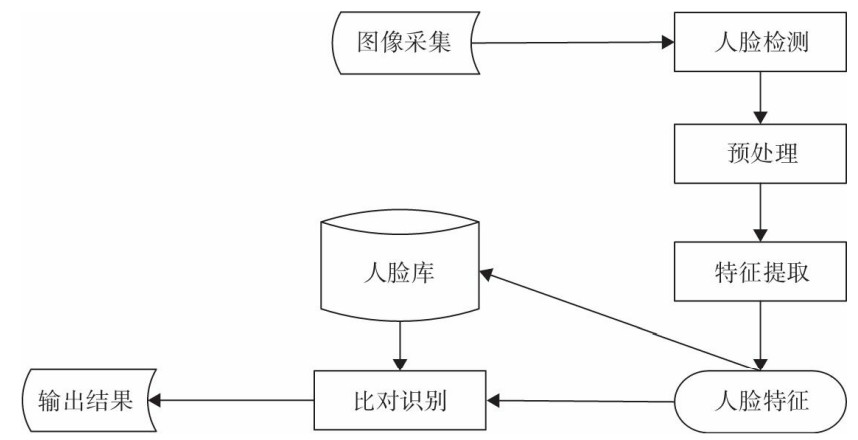
\includegraphics[width=5in]{example/faceDetection.JPG}
\caption{人脸识别的一般处理流程}
\label{figure:3-1}
%\end{minipage}

\end{figure}

其中图像采集包括摄像镜头采集、将已有的图像上传等方式,采集的图像包括静态图像、动态图像、不同位置、不同表情等的图像,当采集对象在设备的拍摄范围内时,采集设备会自动搜索并拍摄人脸图像。影响图像采集的因素很多,主要有图像大小、图像分辨率、光照环境、模糊程度、遮挡程度、采集角度等,这些因素影响图像采集的质量。

由图\href{figure:3-1}{3-1}可知,人脸检测和人脸预处理(人脸对齐)是人脸识别的关键步骤,如果处理效果不好,会直接影响到人脸特征的提取,进而影响最终人脸识别效果。

人脸识别的发展简史主要分成三个阶段\footnote{\url{https://www.jianshu.com/p/639e3f8b7253}}:
\begin{enumerate}
    \item 第一阶段(1950s$\sim$1980s)初级阶段:

    人脸识别被当作一个一般性的模式识别问题,主流技术基于人脸的几何结构特征。这集中体现在人们对于剪影(Profile)的研究上,人们对面部剪影曲线的结构特征提取与分析方面进行了大量研究。人工神经网络也一度曾经被研究人员用于人脸识别问题中。较早从事 AFR 研究的研究人员除了布莱索(Bledsoe)外还有戈登斯泰因(Goldstein)、哈蒙(Harmon)以及金出武雄(Kanade Takeo)等。总体而言,这一阶段是人脸识别研究的初级阶段,非常重要的成果不是很多,也基本没有获得实际应用。

    \item 第二阶段(1990s)高潮阶段:

    这一阶段尽管时间相对短暂,但人脸识别却发展迅速,不但出现了很多经典的方法,例如Eigen Face, Fisher Face和弹性图匹配;并出现了若干商业化运作的人脸识别系统,比如最为著名的 Visionics(现为 Identix)的 FaceIt 系统。  从技术方案上看, 2D人脸图像线性子空间判别分析、统计表观模型、统计模式识别方法是这一阶段内的主流技术。

    \item 第三阶段(1990s末$\sim$现在)

    人脸识别的研究不断深入,研究者开始关注面向真实条件的人脸识别问题,主要包括以下四个方面的研究:1)提出不同的人脸空间模型,包括以线性判别分析为代表的线性建模方法,以Kernel 方法为代表的非线性建模方法和基于3D信息的3D人脸识别方法。2)深入分析和研究影响人脸识别的因素,包括光照不变人脸识别、姿态不变人脸识别和表情不变人脸识别等。3)利用新的特征表示,包括局部描述子(Gabor Face, LBP Face 等)和深度学习方法。4)利用新的数据源,例如基于视频的人脸识别和基于素描、近红外图像的人脸识别。
\end{enumerate}

\subsection{人脸检测}

\subsubsection{经验驱动特征}

1、梯度方向直方图(HoG)特征

2、Haar特征

3、SIFT特征

4、局部二值模式(LBP)特征

\subsubsection{人脸检测算法}

1、霍夫变换

2、Gabor变换

3、频繁模式挖掘算法

4、Viola-Jones算法

\href{https://www.baidu.com/link?url=2oqh2YAsm7N9MPmaWNQzN7WFegwFHwwfzgx4c1pFFK35O9L7t9bRZBfBpBHtV-CDe7uGBrEmM5T0I2XkjL0mK4OIviXPMcH1iji6cENkFou&wd=&eqid=ae2017260000261f00000004604eb76d}

\href{https://blog.csdn.net/matrix_space/article/details/53840740}

\subsubsection{深度学习模型}

1、YOLO

2、Faster RCNN

\subsection{人脸对齐}

\subsubsection{人脸对齐的研究进展}

\subsubsection{人脸对齐算法研究概述}

同一个人在不同的图像序列中可能呈现出不同的姿态和表情,这种情况是不利于人脸识别的。所以有必要将人脸图像都变换到一个统一的角度和姿态,这就是人脸对齐,又称人脸关键点定位,它的原理是找到人脸的若干个关键点(基准点、如眼角、鼻尖、嘴角等),然后利用这些对应的关键点通过相似变换(SimilarityTransform,旋转、缩放和平移)将人脸尽可能变换到标准人脸。作为人脸识别的预处理操作,人脸对齐在人脸检测的基础上处理过程如图\href{figure:3-2}{3-2}所示。人脸对齐的结果可以用于:
人脸验证, 人脸识别(Face recognition),属性计算(Attribute computing),表情识别(Expression recognition), 姿态估计(Pose Estimation) 等
\footnote{\url{https://www.jianshu.com/p/e4b9317a817f}}。

\begin{figure}[!htp]

\centering
%\begin{minipage}[t]{5in}
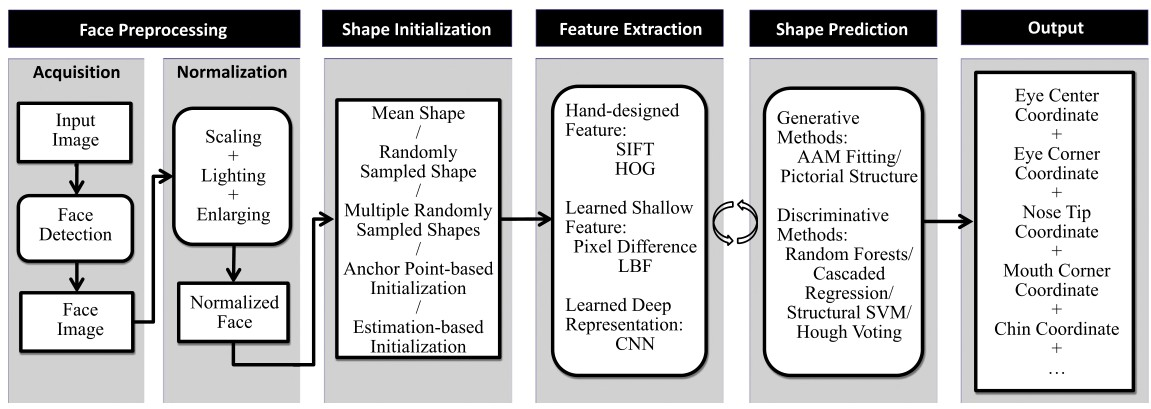
\includegraphics[width=5.5in]{example/faceAligment.JPG}
\caption{人脸对齐的一般处理流程}
\label{figure:3-2}
%\end{minipage}

\end{figure}

综合考虑传统方法和目前最新进展,从技术实现上可将人脸关键点检测分为2 大类:生成式方法(Generative methods) 和 判别式方法(Discriminative methods)。
Generative methods 构建人脸shape和appearance的生成模型。这类方法将人脸对齐看作是一个优化问题,来寻找最优的shape 和appearance 参数,使得appearance模型能够最好拟合输入的人脸。这类方法包括:

\begin{itemize}
    \item AAM (Active Appearnce Model)
    \item ASM(Active Shape Model)
\end{itemize}

Discriminative methods直接从appearance推断目标位置。这类方法通常通过学习独立的局部检测器或回归器来定位每个面部关键点,然后用一个全局的形状模型对预测结果进行调整,使其规范化。或者直接学习一个向量回归函数来推断整个脸部的形状。这类方法包括传统的方法以及最新的深度学习方法,具体分为如下几种经典的实现方式:

\begin{itemize}
    \item Constrained local models (CLMs)
    \item Deformable part models (DPMs)
    \item 基于级联形状回归的方法(Cascaded regression)
    \item 基于深度学习的方法
\end{itemize}

从空间维度来考虑,以上这些方法又可分为2D方法,3D方法,稀疏方法和密集方法等。需要指出的是,由于深度学习方法可以很好的实现对多任务的处理,因此有很多新的算法可以同时完成对2D关键点和3D 关键点的同时获取,进而可进一步支持后续的多任务分析,如人脸对齐,3D姿态分析等。

在人脸关键点定位的发展史上,具有里程碑式的有如下五种方法:
\begin{itemize}
	\item 1995 年,Cootes 的 ASM(Active Shape Model)。
	\item 1998 年,Cootes 的 AAM(Active Appearance Model) 算法。
	\item 2006 年,Ristinacce 的 CLM(Constrained Local Model)算法。
    \item 2010 年,Rollar 的 cascaded Regression 算法。
    \item 2013 年,香港中文大学的汤晓欧和Sun Yi等开创深度学习人脸关键点检测的先河,首次将 CNN 应用到人脸关键点定位上。
\end{itemize}

接下来主要介绍2D人脸对齐算法和模型

\subsubsection{人脸对齐算法}

1、LBF算法

\subsubsection{MTCNN}

MTCNN是中国科学院深圳研究所在2016年论文(Joint Face Detection and Alignment using Multi-task Cascaded Convolutional Networks) 中提出的一个多任务级联卷积神经网络,它可以用来做人脸检测和人脸对齐,并且人脸检测和人脸对齐是同时进行的。在MTCNN 中,它使用了3 级CNN 级联,包括三个部分PNet,RNet, ONet。

该模型的特征跟HAAR级联检测在某些程度上有一定的相通之处,都是采用了级联方式,都是在初期就拒绝了绝大多数的图像区域,有效的降低了后期CNN网络的计算量与计算时间。MTCNN模型主要贡献在于:

\begin{enumerate}[label=\circled{\arabic*}]
    \item 提供一种基于CNN方式的级联检测方法,基于轻量级的CNN 模型就实现了人 脸检测与点位标定,而且性能实时。
    \item 实现了对难样本挖掘在线训练提升性能
    \item 一次可以完成多个任务。
\end{enumerate}


1、MTCNN基本流程\footnote{MTCNN工作原理 \url{https://blog.csdn.net/qq_36782182/article/details/83624357}}:

1)构建图像金字塔

首先将图像进行不同尺度的变换,构建图像金字塔,以适应不同大小的人脸的进行检测。

2)P-Net

全称为Proposal Network,其基本的构造是一个全卷积网络。对上一步构建完成的图像金字塔,通过一个FCN进行初步特征提取与标定边框,并进行Bounding-Box Regression调整窗口与NMS 进行大部分窗口的过滤。

P-Net是一个人脸区域的区域建议网络,该网络的将特征输入结果三个卷积层之后,通过一个人脸分类器判断该区域是否是人脸,同时使用边框回归和一个面部关键点的定位器来进行人脸区域的初步提议,该部分最终将输出很多张可能存在人脸的人脸区域,并将这些区域输入R-Net 进行进一步处理。

这一部分的基本思想是使用较为浅层、较为简单的CNN快速生成人脸候选窗口。

\begin{figure}[!htp]

\centering
%\begin{minipage}[t]{5in}
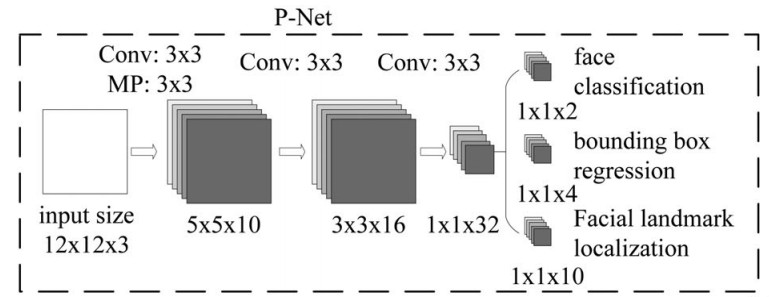
\includegraphics[width=4in]{example/p_net.jpg}
\caption{P-Net实现细节}
\label{figure:3-2}
%\end{minipage}

\end{figure}

3)R-Net

全称为Refine Network,其基本的构造是一个卷积神经网络,相对于第一层的P-Net来说,增加了一个全连接层,因此对于输入数据的筛选会更加严格。在图片经过P-Net后,会留下许多预测窗口,我们将所有的预测窗口送入R-Net,这个网络会滤除大量效果比较差的候选框,最后对选定的候选框进行Bounding-Box Regression和NMS进一步优化预测结果。

因为P-Net的输出只是具有一定可信度的可能的人脸区域,在这个网络中,将对输入进行细化选择,并且舍去大部分的错误输入,并再次使用边框回归和面部关键点定位器进行人脸区域的边框回归和关键点定位,最后将输出较为可信的人脸区域,供O-Net使用。对比与P-Net使用全卷积输出的1$\times$1$\times$32的特征,R-Net使用在最后一个卷积层之后使用了一个128的全连接层,保留了更多的图像特征,准确度性能也优于P-Net。

R-Net的思想是使用一个相对于P-Net更复杂的网络结构来对P-Net生成的可能是人脸区域区域窗口进行进一步选择和调整,从而达到高精度过滤和人脸区域优化的效果。
\begin{figure}[!htp]

\centering
%\begin{minipage}[t]{5in}
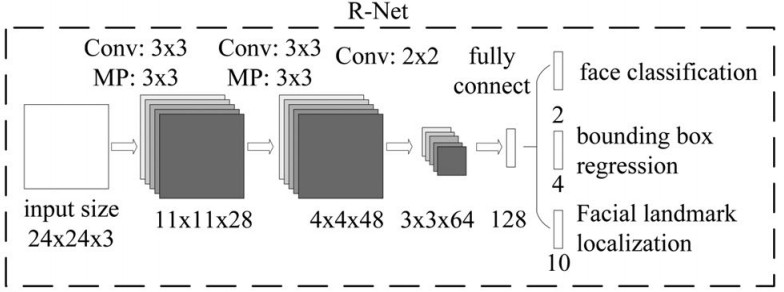
\includegraphics[width=4in]{example/R_net.jpg}
\caption{R-Net实现细节}
\label{figure:3-2}
%\end{minipage}

\end{figure}

4)O-Net

全称为Output Network,基本结构是一个较为复杂的卷积神经网络,相对于R-Net来说多了一个卷积层。O-Net的效果与R-Net的区别在于这一层结构会通过更多的监督来识别面部的区域,而且会对人的面部特征点进行回归,最终输出五个人脸面部特征点。

是一个更复杂的卷积网络,该网络的输入特征更多,在网络结构的最后同样是一个更大的256的全连接层,保留了更多的图像特征,同时再进行人脸判别、人脸区域边框回归和人脸特征定位,最终输出人脸区域的左上角坐标和右下角坐标与人脸区域的五个特征点。O-Net拥有特征更多的输入和更复杂的网络结构,也具有更好的性能,这一层的输出作为最终的网络模型输出。

\begin{figure}[!htp]

\centering
%\begin{minipage}[t]{5in}
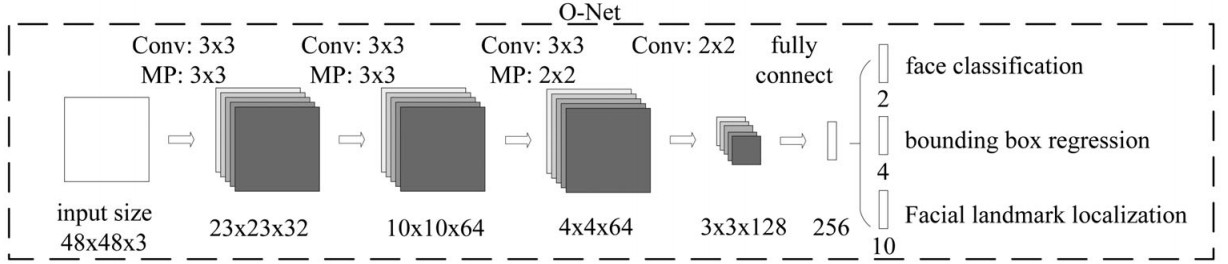
\includegraphics[width=5in]{example/O_net.jpg}
\caption{O-Net实现细节}
\label{figure:3-2}
%\end{minipage}

\end{figure}

MTCNN基本流程如图\href{figure:3-2}{3-2}所示。

\begin{figure}[!htp]

\centering
%\begin{minipage}[t]{5in}
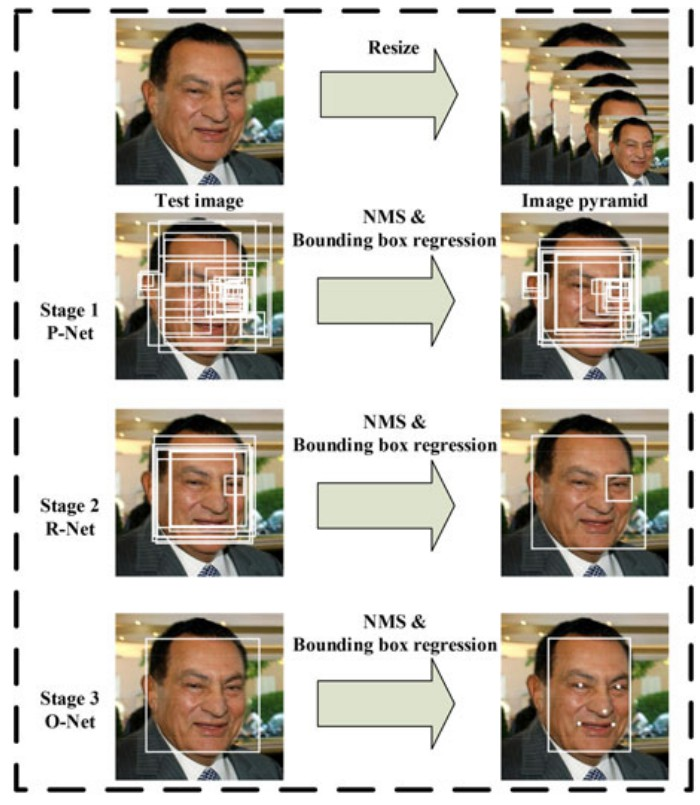
\includegraphics[width=4in]{example/MTCNN.JPG}
\caption{MTCNN基本流程}
\label{figure:3-2}
%\end{minipage}

\end{figure}

2、网络架构设计

对CNN网络架构,论文作者发现影响网络性能的因素主要原因有两个:
\begin{enumerate}[label=\circled{\arabic*}]
    \item 样本的多样性缺乏会影响网络的鉴别能力;
    \item 相比其它的多类别的分类与检测任务来说,人脸检测是一个二分类,每一层不需要太多filters,也就是说每层网络的feature maps 个数不需要太多;
\end{enumerate}
根据上述两个因素,作者设计网络每层的filter个数有限,但是它增加了整个网络的深度,这样做的好处是可以显著减少计算量,提升整个网络性能,同时全部改用3x3的filter更进一步降低计算量,在卷积层与全连接层使用PReLU作为非线性激活函数(输出层除外)。

3、损失函数 \footnote{MTCNN模型概述 \quad \url{https://blog.51cto.com/gloomyfish/2319246}}

训练这个网络需要如下三任务得到收敛:
\begin{enumerate}[label=\circled{\arabic*}]
    \item 人脸二元分类
    \item BB回归(bounding box regression)
    \item 标记定位(Landmark localization)
\end{enumerate}

1)交叉熵损失

训练时候对于人脸采用交叉熵损失如下式所示。其中$p_i$表示样本$x_i$ 是人脸的概率,$y_i^{det} \in {0,1}$表示标注标签。
\begin{align}
& L_i^{det} = -(y_i^{det} log(p_i) + (1 - y_i^{det})(1 - log(p_i)))
\end{align}

2)BB回归损失

对每个候选窗口,计算它与标注框之间的offset,目标是进行位置回归,计算其平方差损失如下式所示。
\begin{align}
& L_i^{box} = ||\hat{y}_i^{box} - y_i^{box}||_2^2
\end{align}

其中$\hat{y}_i^{box}$为回归框,${y}_i^{box}$为标注框。

3)脸部landmark位置损失:
\begin{align}
& L_i^{landmark} = ||\hat{y}_i^{landmark} - y_i^{landmark}||_2^2
\end{align}
其中$\hat{y}_i^{landmark}$网络输出,$y_i^{landmark}$是标注点位置。

总计有五个点位坐标分别为左眼、右眼、鼻子、左嘴角、右嘴角。

4)总训练损失

因为每个CNN网络完成不同的训练任务,所以在网络学习/训练阶段需要不同类型的训练数据。所以在计算损失的时候需要区别对待,对待背景区域,在R-Net 与O-Net中的训练损失为0,因为它没有包含人脸区域,通过参数beta=0 来表示这种类型。总的训练损失可以表示如下:
\begin{align}
& \min \sum_{i = 1}^N \sum_{j \in \{det,box,landmark\}} \alpha_j \beta_i^j L_i^j
\end{align}

其中$\alpha_j$表示任务权重,在P-Net与R-Net中$\alpha_{det} = 1.0$,$\alpha_{box} = 0.5$,$\alpha_{landmark} = 0.5$。在O-Net 中$\alpha_{det} = 1.0$,$\alpha_{box} = 0.5$,$\alpha_{landmark} = 1.0$。$\beta_i^j \in {0,1}$表示样本类型权重。
在P-Net中对人脸进行二元分类时候就可以在线进行难样本挖掘,在网络前向传播时候对每个样本计算得到的损失进行排序(从高到低)然后选择70$\%$进行反向传播,原因在于好的样本对网络的性能提升有限,只有那些难样本才能更加有效训练,进行反向传播之后才会更好的提升整个网络的人脸检测准确率。作者的对比实验数据表明这样做可以有效提升准确率。在训练阶段数据被分为四种类型:
\begin{itemize}
    \item 负样本:并交比小于0.3
    \item 正样本:并交比大于0.65
    \item 部分脸:并交比在0.4~0.65之间
    \item Landmark脸:能够找到五个landmark位置的
\end{itemize}

其中在负样本与部分脸之间并没有明显的差异鸿沟,作者选择0.3与0.4 作为区间。正负样本被用来实现人脸分类任务训练;正样本与部分脸样本训练BB回归;Landmark脸用来训练人脸五个点位置定位。所以整个训练数的比例如下:负样本:正样本:部分脸:landmark脸=3:1:1:2。

从P-Net到R-Net,再到最后的O-Net,网络输入的图像越来越大,卷积层的通道数也越来越多,网络的深度也越来越深,因此识别人脸的准确率也越来越高。同时P-Net网络的运行速度较快,R-Net次之、O-Net 运行速度最慢。之所以使用这3个网络,是因为一开始如果直接对图像使用O-Net网络,速度会非常慢。实际上P-Net 先做了一层过滤,将过滤后的结果再交给R-Net 进行过滤,最后将过滤后的结果交给效果最好但是速度最慢的O-Net 进行识别。这样在每一步都提前减少了需要判别的数量,有效地降低了计算时间,从而大大提高运行效率。人脸检测以后,接下来就特征提取。

\section{人脸表情识别}

\subsection{AUs和基本表情}

\subsubsection{面部动作单元(AUs)}

图\href{fig:4-8}{4-8}涵盖了人脸的大部分肌肉,这些肌肉是我们在后面的AU介绍里要提到的。为了方便下面的学习,我们可以先了解下这些肌肉的名字以及在脸上出现的位置 \footnote{\url{http://www.360doc.com/content/15/0128/13/10690471_444446832.shtml}}。

\begin{figure}[!htp]
\centering
%\begin{minipage}[t]{5in}
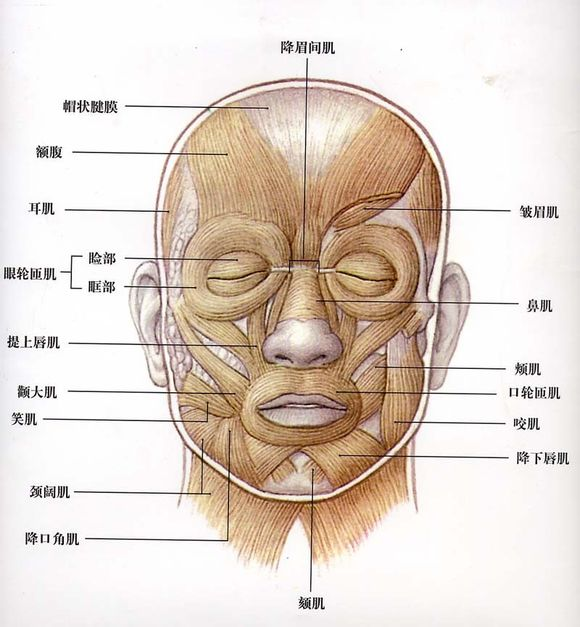
\includegraphics[width=4in]{example/AUExp1.jpg}
\caption{人脸肌肉分布图}
\label{figure:4-8}
%\end{minipage}
\end{figure}

面部动作编码系统(FACS),是一种基于最初由瑞典解剖学家Carl-HermanHjortsj联开发的系统,通过面部外观对人类面部动作进行分类。后来由Paul Ekman和Wallace V.Friesen采用,并作了深入的研究,通过观察和生物反馈,描绘出不同的脸部肌肉动作和不同表情的对应关系,并于1978年出版。

面部动作编码系统(FACS),根据人脸的解剖学特点,可将其划分成若干既相互独立又相互联系的动作单元(Action Units,AU),这些面部动作单元的运动特征及其所控制的主要区域可以反映出面部表情。FACS中常见动作单元详解如表\href{tab:4-1}{4-1}所示 \footnote{微表情分析师FACS动作单元详解 \quad \url{http://www.360doc.com/content/16/0130/20/12057352_531731091.shtml}}。

\begin{table}[]
\centering
\caption{FACS中常见动作单元详解}
\begin{tabular}{|l|l|l|l|l|l|}
\hline
\textbf{编码} &
  \textbf{运动部位} &
  \textbf{常见情绪} &
  \textbf{编码} &
  \textbf{运动部位} &
  \textbf{常见情绪} \\ \hline
\textbf{AU1} &
  \begin{tabular}[c]{@{}l@{}}额腹(额肌)的内侧\\ 收缩上拉\end{tabular} &
  \begin{tabular}[c]{@{}l@{}}惊讶、恐惧、\\ 悲伤\end{tabular} &
  \textbf{AU15} &
  降口角肌 &
  悲伤、不满 \\ \hline
\textbf{AU2} &
  额肌的外侧收缩 &
  惊讶、恐惧 &
  \textbf{AU16} &
  降下唇肌 &
  常表现为尴尬 \\ \hline
\textbf{AU4} &
  \begin{tabular}[c]{@{}l@{}}降眉间肌和皱眉肌的组合\\ 肌肉群\end{tabular} &
  恐惧、愤怒 &
  \textbf{AU17} &
  颏肌 &
  \begin{tabular}[c]{@{}l@{}}生气、不满、\\ 轻蔑\end{tabular} \\ \hline
\textbf{AU5} &
  \begin{tabular}[c]{@{}l@{}}抬起上眼皮(上眼脸\\ 提肌)上眼脸减少\\ 或消失,使更多的虹膜\\ 暴露(眼睛瞪大)\end{tabular} &
  \begin{tabular}[c]{@{}l@{}}惊讶、专注、\\ 恐惧、愤怒\end{tabular} &
  \textbf{AU18} &
  口轮匝肌 &
  \begin{tabular}[c]{@{}l@{}}无具体情绪\\ 表现\end{tabular} \\ \hline
\textbf{AU6} &
  眼轮匝肌外圈的运动 &
  轻蔑、微笑 &
  \textbf{AU20} &
  笑肌 &
  恐惧 \\ \hline
\textbf{AU7} &
  眼轮匝肌内圈收缩 &
  怀疑、愤怒 &
  \textbf{AU22} &
  口轮匝肌 &
  厌恶、愤怒 \\ \hline
\textbf{AU9} &
  皱起鼻肌 &
  \begin{tabular}[c]{@{}l@{}}厌恶、讨厌\\ (有些女生用\\ AU9来撒娇)\end{tabular} &
  \textbf{AU23} &
  口轮匝肌 &
  \begin{tabular}[c]{@{}l@{}}愤怒、不满、\\ 生气\end{tabular} \\ \hline
\textbf{AU10} &
  上唇方肌上拉 &
  \begin{tabular}[c]{@{}l@{}}厌恶、不屑、\\ 鄙视、愤怒\end{tabular} &
  \textbf{AU24} &
  口轮匝肌 &
  不安、焦虑 \\ \hline
\textbf{AU11} &
  颧小肌 &
  \begin{tabular}[c]{@{}l@{}}强调表情强度、\\ 辨识真假笑\end{tabular} &
  \textbf{AU25} &
  嘴唇张开 &
  疑惑 \\ \hline
\textbf{AU12} &
  颧小肌和颧大肌 &
  愉快或假笑 &
  \textbf{AU26} &
  \begin{tabular}[c]{@{}l@{}}嘴唇、牙齿\\ 分离\end{tabular} &
  惊讶 \\ \hline
\textbf{AU13} &
  提口角肌 &
  \begin{tabular}[c]{@{}l@{}}辅助AU12、\\ AU11运动\end{tabular} &
  \textbf{AU27} &
  \begin{tabular}[c]{@{}l@{}}下颌骨被向\\ 下拉,改变嘴\\ 部打开的形状,\\ 从一个水平的椭圆\\ 变成了竖直的椭圆。\end{tabular} &
  无具体情绪 \\ \hline
\textbf{AU14} &
  颊肌 &
  \begin{tabular}[c]{@{}l@{}}多数表现为\\ 没自信\end{tabular} &
  \textbf{AU28} &
  吸唇 &
  担忧、犹豫 \\ \hline
\end{tabular}
\end{table}

目前,随着计算机技术和信息技术的发展,深度学习技术得到了广泛的应用。业内在AU识别方面,大多是收集大量AU样本,搭建卷积神经网络训练出AU特征识别模型,进而用来进行AU特征识别与分类,但该种方法对样本库样本质量和数量要求较高,调参时间长,且准确率不高。尤其是有些存在互斥关系或递进关系的AU,关系界定不清,很容易出现耦合,导致识别错误。

此外,面部动作单元的肌肉的动作程度,也称AU强度,其幅值的大小也取决于被识别者的天生的相貌特征,不同相貌的人即使做同样的肌肉动作,所呈现的AU强度也可能不同,这势必会导致识别出的AU强度有所差异,图\href{fig:4-1}{4-1}展示了AU4在不同强度下的人脸表情。因此有必要设置一个初始化环节用来均衡由于人的相貌所导致的差异。但是现有的AU识别算法鲜有该环节的设置,即会导致在识别初期便引入识别误差,进一步,导致后续任何基于面部动作单元(AU)所开展的工作,如表情识别、微表情识别、状态识别等环节识别失误的加剧
\footnote{一种面部动作单元的识别方法、系统与流程 \quad \url{http://www.xjishu.com/zhuanli/55/201910184196.html}}。

\begin{figure}[t]
\centering
    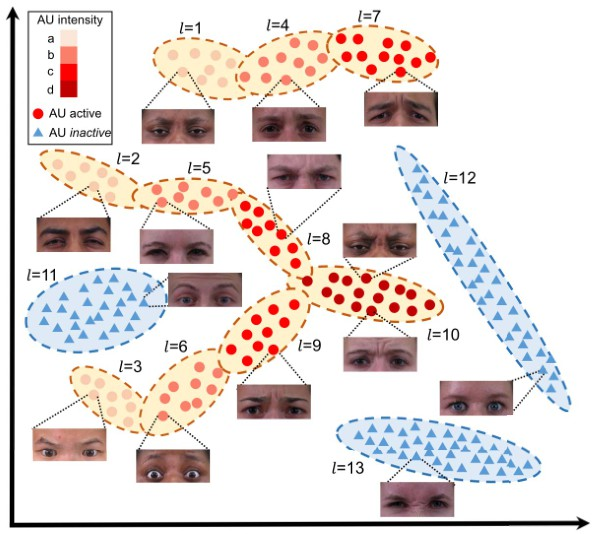
\includegraphics[width=4in]{example/AU4.JPG}
    \caption{AU4强度分类}
    \label{fig:3-1}
\end{figure}

\subsubsection{人脸表情数据集}

对于人类情感的识别主要有两种方法:一种是通过摄像机捕捉面部特征进行表情识别,另一种是通过获取受试者的生物电信号(ECG,EEG,PPG)进行情感的识别。对于前者,计算机将表情识别转化成有监督的分类问题,而对于后者,计算机将情感识别转化成回归问题,如图\href{fig:4-2}{4-2} 所示。

\begin{figure}[t]
\centering
    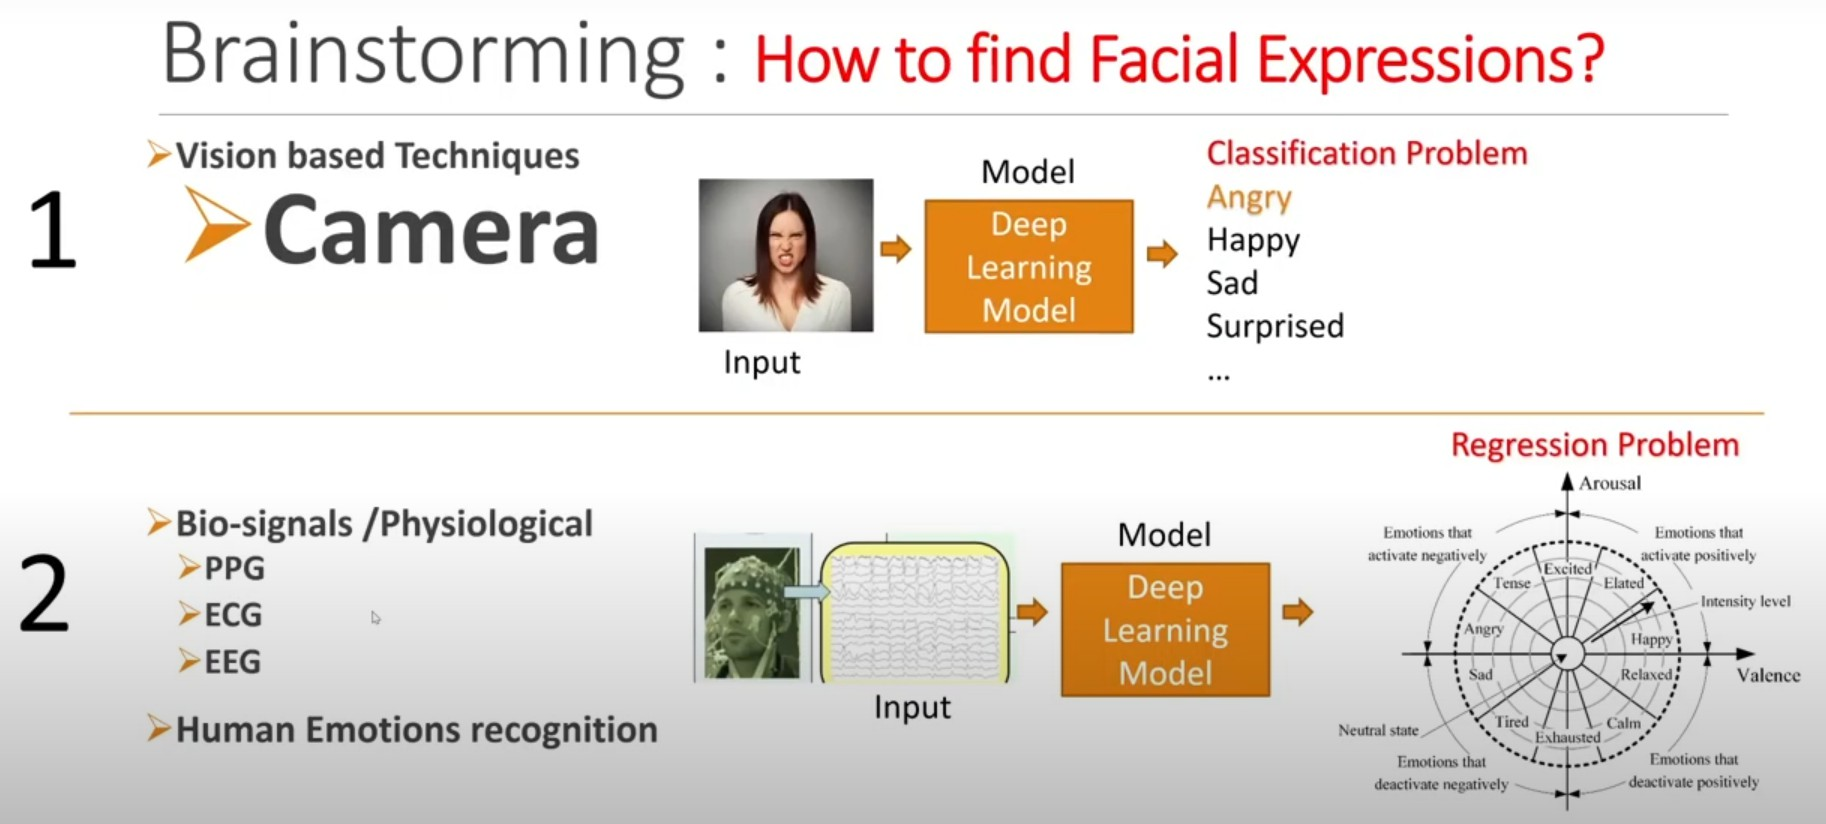
\includegraphics[width=5in]{example/FER.jpg}
    \caption{情感识别技术}
\end{figure}

常见的面部表情识别数据集

1、FER 2013和FER+数据集

FER 2013包含共26190张48*48灰度图,图片的分辨率比较低,含7类表情:生气(angry),厌恶(disgusting),恐惧(Fear),开心(happy),伤心(sad),惊喜(surprised)和中立(neutral)。在FER 2013训练集,测试集中,各标签样本数如表\href{table:1-2}{1-2}所示。但是该数据集存在以下一些问题:
\begin{itemize}
	\item 样本不均衡:数据集存在正负样本、难易样本、类别间样本这3种不均衡问题。常用的解决方法是使用GAN实现数据增强。
	\item 类内差异(intra-class variation):一类物体的个体之间的外形差异很大,比如椅子。这一类物体有许多不同的对象,每个都有自己的外形。可以通过避免过拟合的方法(正则化损失函数,批量归一化等) 来解决这个问题。
	\item 遮挡问题(Occlusion):比如头发,肢体等遮挡了面部,导致面部部分信息丢失。
    \item 是否戴眼镜:部分样本的面部表情特征被眼镜遮挡。
\end{itemize}

\begin{table}[]
\caption{FER 2013数据集}
\centering
\resizebox{\textwidth}{!}{%
\begin{tabular}{|l|l|l|l|l|l|c|l|}
\hline
FER 2013 & 0=Angry & 1=Disgust                  & 2=Fear & 3=Happy                     & 4=Sad & \multicolumn{1}{r|}{5=Surprise} & 6=Neutral \\ \hline
Training & 3995    & {\color[HTML]{FE0000} 436} & 4096   & {\color[HTML]{FE0000} 7214} & 4830  & 3171                            & 4965      \\ \hline
Testing  & 958     & 111                        & 1024   & 1774                        & 1247  & 831                             & 1232      \\ \hline
\end{tabular}%
}
\label{table:1-2}
\end{table}

因此就有了后来微软重新标注的FER2013 plus(FER+)数据集 \\

2、KDEF与AKDEF(karolinska directed emotional faces)数据集\footnote{【技术综述】人脸表情识别研究技术综述 \quad \url{https://zhuanlan.zhihu.com/p/40572244}}

这个数据集最初是被开发用于心理和医学研究目的。它主要用于知觉,注意,情绪,记忆等实验。在创建数据集的过程中,特意使用比较均匀,柔和的光照,被采集者身穿统一的T恤颜色。这个数据集,包含70个人,35个男性,35个女性,年龄在20至30岁之间。没有胡须,耳环或眼镜,且没有明显的化妆。7种不同的表情,每个表情有5个角度。总共4900张彩色图。尺寸为562*762像素,官网地址如下:\href{https://www.emotionlab.se/publi/}{Emotion Lab at Karolinska Institutet}。\\

3、RaFD数据集

该数据集是Radboud大学Nijmegen行为科学研究所整理的,这是一个高质量的脸部数据库,总共包含67个模特:20名白人男性成年人,19名白人女性成年人,4个白人男孩,6个白人女孩,18名摩洛哥男性成年人。总共8040张图,包含8种表情,即愤怒,厌恶,恐惧,快乐,悲伤,惊奇,蔑视和中立。每一个表情,包含3个不同的注视方向,且使用5个相机从不同的角度同时拍摄的,官网地址如下:\href{http://www.socsci.ru.nl:8180/RaFD2/RaFD?p=main}{Radboud Faces Database}。\\

4、CelebFaces Attributes Dataset (CelebA)数据集

该数据集是商汤科技的一个用于研究人脸属性的数据集,一个包含超过200K名人图像的大型人脸属性数据集,每个数据集都有40个属性注释。该数据集中的图像涵盖了大型姿态变化和复杂背景。CelebA的多样性非常好,有约10万张带微笑属性的数据。数据集下载地址:
\href{https://mp.weixin.qq.com/s?__biz=MzU1NDMwMjE3Mw==&mid=2247484102&idx=1&sn=e6bdde7a694d101e9a335f6b41b1ecc6&chksm=fbe4ed74cc9364629da8d866c6787456863c868adfaceba3fcb9b337fb4e03f37cc3bdb9291f&token=2099057174&lang=zh_CN#rd}{CelebA 数据集}

\subsection{传统研究方法}

表情特征提取主要采用数学方法,是依靠计算机技术对人脸表情的数字图像进行数据的组织和处理,提取表情特征,去除非表情噪声的方法。在某些情况下,特征提取算法提取了图像的主要特征,客观上降低了图像的维数,因此这些特征提取算法也具有降维的作用\footnote{【技术综述】人脸表情识别研究技术综述 \quad \url{https://zhuanlan.zhihu.com/p/40572244}}。

人脸表情的产生是一个很复杂的过程,如果不考虑心理和环境因素,呈现在观察者面前的就是单纯的肌肉运动,以及由此带来的面部形体和纹理的变化。静态图像呈现的是表情发生时单幅图像的表情状态,动态图像呈现的是表情在多幅图像之间的运动过程。因此根据表情发生时的状态和处理对象来区分,表情特征提取算法大体分为基于静态图像的特征提取方法和基于动态图像的特征提取方法。其中基于静态图像的特征提取算法可分为整体法和局部法,基于动态图像的特征提取算法又分为光流法、模型法和几何法。

\subsubsection{基于静态图像的特征提取方法}

1、整体法

人脸表情依靠肌肉的运动来体现。人脸表情静态图像直观地显示了表情发生时人脸肌肉运动所产生的面部形体和纹理的变化。从整体上看,这种变化造成了面部器官的明显形变,会对人脸图像的全局信息带来影响,因此出现了从整体角度考虑表情特征的人脸表情识别算法。

整体法中的经典算法包括主元分析法(PCA)、独立分量分析法(ICA)和线性判别分析法(LDA)。研究者针对于此也做了大量的工作,文献
\cite{renlianbiaoqingshibie},\cite{jiyuICAyu}, \cite{renlianbiaoqingshibie1}采用FastICA 算法提取表情特征,该方法不但继承了ICA算法能够提取像素间隐藏信息的特点,而且可以通过迭代,快速地完成对表情特征的分离。文献\cite{zhichixiangliangjianbie}提出了支持向量鉴别分析(SVDA)算法,该算法以Fisher线性判别分析和支持向量机基础,能够在小样本数据情况下,使表情数据具有最大的类间分离性,而且不需要构建SVM算法所需要的决策函数。实验证明了该算法的识别率高于PCA和LDA。文献\cite{ma2001facial}依靠二维离散余弦变换,通过频域空间对人脸图像进行映射,结合神经网络实现对表情特征的分类。

2、局部法

静态图像上的人脸表情不仅有整体的变化,也存在局部的变化。面部肌肉的纹理、皱褶等局部形变所蕴含的信息,有助于精确地判断表情的属性。局部法的经典方法是Gabor小波法和LBP 算子法。文献\cite{kyperountas2010salient}以Gabor小波等多种特征提取算法为手段,结合新的分类器对静态图像展开实验。文献\cite{zheng2006facial}首先人工标记了34个人脸特征点,然后将特征点的Gabor小波系数表示成标记图向量,最后计算标记图向量和表情语义向量之间的KCCA系数,以此实现对表情的分类。文献\cite{Fuxiaofen0}提出了CBP算子法,通过比较环形邻域的近邻点对,降低了直方图的维数。针对符号函数的修改,又增强了算法的抗噪性,使CBP算子法取得了较高的识别率。

\subsubsection{基于动态图像的特征提取方法}

动态图像与静态图像的不同之处在于:动态图像反映了人脸表情发生的过程。因此动态图像的表情特征主要表现在人脸的持续形变和面部不同区域的肌肉运动上。目前基于动态图像的特征提取方法主要分为光流法、模型法和几何法。

1、光流法

光流法是反映动态图像中不同帧之间相应物体灰度变化的方法。早期的人脸表情识别算法多采用光流法提取动态图像的表情特征,这主要在于光流法具有突出人脸形变、反映人脸运动趋势的优点。因此该算法依旧是传统方法中来研究动态图像表情识别的重要方法。文献\cite{yacoob1996recognizing}首先采用连续帧之间的光流场和梯度场,分别表示图像的时空变化,实现每帧人脸图像的表情区域跟踪;然后通过特征区域运动方向的变化,表示人脸肌肉的运动,进而对应不同的表情。

2、模型法

人脸表情识别中的模型法是指对动态图像的表情信息进行参数化描述的统计方法。常用算法主要包括主动形状模型法(ASM)和主动外观模型法(AAM),两种算法都可分为形状模型和主观模型两部分。就表观模型而言,ASM反映的是图像的局部纹理信息,而AAM反映的是图像的全局纹理信息。文献\cite{tsalakanidou2010real}提出了基于ASM的三维人脸特征跟踪方法,该方法对人脸81个特征点进行跟踪建模,实现了对部分复合动作单元的识别。文献\cite{wang2007static}借助图像的地形特征模型来识别人脸动作和表情;利用AAM和人工标记的方法跟踪人脸特征点,并按照特征点取得人脸表情区域;通过计算人脸表情区域的地形直方图来获得地形特征,从而实现表情识别。文献\cite{sung2008pose}提出了基于二维表观特征和三维形状特征的AAM算法,在人脸位置发生偏移的环境下,实现了对表情特征的提取。

3、几何法

在表情特征提取方法中,研究者考虑到表情的产生与表达在很大程度上是依靠面部器官的变化来反映的。人脸的主要器官及其褶皱部分都会成为表情特征集中的区域。因此在面部器官区域标记特征点,计算特征点之间的距离和特征点所在曲线的曲率,就成为了采用几何形式提取人脸表情的方法。文献\cite{kotsia2006facial}使用形变网格对不同表情的人脸进行网格化表示,将第一帧与该序列表情最大帧之间的网格节点坐标变化作为几何特征,实现对表情的识别。

\subsubsection{表情特征的分类}

特征分类的目的是判断特征所对应的表情类别。在人脸表情识别中,表情的类别分为两部分:基本表情和动作单元。前者一般适用于所有的处理对象,后者主要适用于动态图像,可以将主要的特征分类方法分为基于贝叶斯网络的分类方法和基于距离度量的分类方法。

1、基于贝叶斯网络的分类方法

贝叶斯网络是以贝叶斯公式为基础、基于概率推理的图形化网络。从人脸表情识别的角度出发,概率推理的作用就是从已知表情信息中推断出未知表情的概率信息的过程。基于贝叶斯网络的方法包括各种贝叶斯网络分类算法和隐马尔科夫模型(HMM)算法。文献\cite{cohen2003facial}研究者 分别采用了朴素贝叶斯(NB)分类器、树增强器(TAN)和HMM实现表情特征分类。

2、基于距离度量的分类方法

基于距离度量的分类方法是通过计算样本之间的距离来实现表情分类的。代表算法有近邻法和SVM算法。近邻法是比较未知样本x与所有已知类别的样本之间的欧式距离,通过距离的远近来决策x与已知样本是否同类;SVM算法则是通过优化目标函数,寻找到使不同类别样本之间距离最大的分类超平面。文献\cite{Fuxiaofen0}采用了最近邻法对表情特征进行分类,并指出最近邻法的不足之处在于分类正确率的大小依赖于待分类样本的数量。\cite{XuWenhui2009},\cite{XuQinZhen2008}分别从各自角度提出了对SVM 的改进,前者将k近邻法与SVM结合起来,把近邻信息集成到SVM的构建中,提出了局部SVM 分类器;后者提出的CSVMT 模型将SVM和树型模块结合起来,以较低的算法复杂度解决了分类子问题。

\subsubsection{其他}

相比于生理信号,通过面部表情进行情感识别是最为直接的方式,表情描述特征主要分为基于静态图片和动态视频两类。目前比较经典的静态表情描述特征有局部二值模式(LBP), 梯度方向直方图(HOG)和Gabor 特征等,虽然对于静态的表情识别,可以取得较好效果,但是静态图片仅是对表情某瞬间的捕捉,无法
描述表情的动态变化过程,因此,基于动态视频的情感识别逐渐得到研究学者的关注。Zhao等人提出LBP-TOP(local binary pattern from three orthogonal
planes)时空特征提取方法,该方法可以有效提取图像序列的动态纹理特征。

考虑到静态信息和动态信息在特征描述上的互补性,Zhao等人采用LBP-TOP和Gabor多方向直方图融合的方法获取情感特征。Chen等人受LBP-TOP启发提出了梯度方向直方图-3维正交平面(HOG-TOP)特征提取方法,有效地提取了视频图像的边缘和方向信息,并将其与LBP-TOP特征在CK库上作对比,验证其所提方法的有效性。此外,Fan等人利用光流法表示面部运动特征,并结合3维金字塔梯度直方图特征(PHOG-TOP) 实现情感判别,取得了不错的效果。

虽然面部表情看起来可以直观地显示情感的变化,但是许多内在的情感变化过程并没有伴随视觉的面部活动被感知,人们可以掩饰和隐藏他们的情感体验,使观察者误会表情的含义。同时基于面部表情图像的特征提取方法大多基于灰度图像,在彩色图像转换为灰度图像的过程中,也会丢失部分信息。对视觉表情不足之处一个好的弥补方法是通过生理信号来分析人体潜在的情感状态。大量的研究表明,情感具有生理可分性。王蓓等人对面部表情和生理信号分别进行特征层融合和决策层融合,并将两种融合结果作对比,实验结果表明在两种模态信息量差异明显的情况下,基于特征层融合的双模态情感识别方法效果不如决策层融合理想。

Tsai等人从皮肤电、手指温度和心率信号中提取生理特征,然后结合12 种面部表情特征进行情感判别。Kortelainen等人则采用呼吸频率和心率变异性两路生理信号与面部纹理特征相结合的方法进行双模态情感识别\footnote{融合表情和BVP生理信号的双模态视频情感识别 \quad \url{https://xueshu.baidu.com/usercenter/paper/show?paperid=b22a6ba0c40126662ef983f6c530096d&site=xueshu_se&hitarticle=1}}。

在2018年《\href{https://xueshu.baidu.com/usercenter/paper/show?paperid=b22a6ba0c40126662ef983f6c530096d&site=xueshu_se&hitarticle=1}{融合表情和BVP生理信号的双模态视频情感识别}》一文中,作者在情感特征描述上将LBP-TOP和HOG-TOP两种特征进行融合。其中,LBP-TOP是一种有效的局部纹理描述算子,能够有效地描述图像纹理特征,计算简单,且具有一定的灰度不变性和旋转不变性。HOG-TOP是基于梯度的局部形状描述算子,可以弥补LBP-TOP特征在图像方向和边缘信息特征提取上的缺失,提高表情特征对光照和几何形变的鲁棒性。为了得到增强的BVP生理信号,作者利用颜色放大技术对视频信号进行放大,然后再提取BVP生理信号的情感特征。

在情感分类上,作者首先利用BP神经网络训练两种不同模态的特征,得到不同分类决策信息。然后通过模糊积分融合算法将两种模态得到的分类信息进行决策层融合,最后得到情感识别结果。双模态情感识别系统示意图如图\href{fig:4-8}{4-8}所示。

\begin{figure}[!htp]
\centering
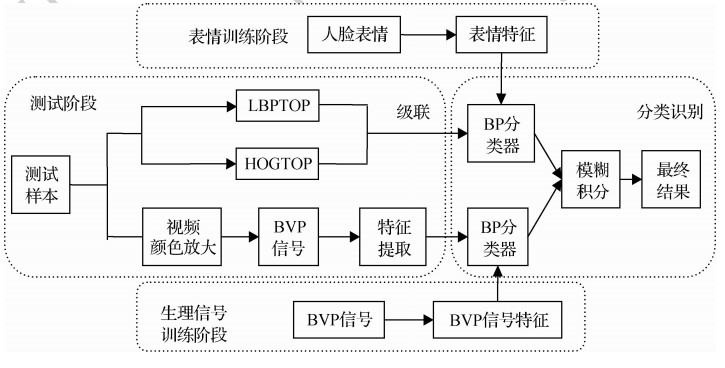
\includegraphics[width=4.5in]{example/BVP_emotion.jpg}
\caption{双模态情感识别系统示意图}
\label{fig1:4-8}
\end{figure}

\subsection{深度学习方法}

上述均为传统研究方法的一些介绍,下文主要讲述如何将深度学习应用到表情识别里,并将以几篇文章为例来详细介绍一下现在深度学习方法的研究方法和思路。

与传统方法特征提取不同,之所以采用深度学习的方法,是因为深度学习中的网络(尤其是CNN)对图像具有较好的提取特征的能力,从而避免了人工提取特征的繁琐,人脸的人工特征包括常用的68个Faciallandmarks等其他的特征,而深度学习除了预测外,往往还扮演着特征工程的角色,从而省去了人工提取特征的步骤。下文首先介绍深度学习中常用的网络类型,然后介绍通过预训练的网络对图像进行特征提取,以及对预训练的网络采用自己的数据进行微调的Fine-Tunning。

如果将深度学习中常用的网络层CNN,RNN,Fully-Connect等层组合成网络,将会产生多种选择,然而这些网络性能的好与坏需要更多地探讨,经过很多研究者的一系列实践,很多网络模型已经具备很多的性能,如ImgeNet比赛中提出模型:AlexNet,GoogleNet(Inception), VGG,ResNet等。这些网络已经经过了ImageNet这个强大数据集的考验,因此在图像分类问题中也常被采用。

对于网络的结构,往往是先通过若干层CNN进行图像特征的提取,然后通过全连接层进行非线性分类,这时的全连接层就类似与MLP,只是还加入了dropout等机制防止过拟合等,最后一层有几个分类就连接几个神经元,并且通过softmax变换得到样本属于各个分类的概率分布。

关于人脸表情识别的讨论一直在继续,很多学者团队都聚焦于此。文献\cite{fabian2016emotionet}提出了用于注释自然情绪面部表情的一百万个图像的大型数据库(即,从因特网下载的面部图像)。首先,证明这个新提出的算法可以跨数据库可靠地识别AU及其强度。根据调研,这是第一个在多个数据库中识别AU及其强度的高精度结果的已发布算法。算法可以实时运行($>$ 30张图像/秒),允许它处理大量图像和视频序列。其次,使用WordNet从互联网下载1,000,000张面部表情图像以及相关的情感关键词。然后通过我们的算法用AU,AU强度和情感类别自动注释这些图像。可以得到一个非常有用的数据库,可以使用语义描述轻松查询计算机视觉,情感计算,社会和认知心理学和神经科学中的应用程序。

文献\cite{fabian2017recognition}提出了一种深度神经体系结构,它通过在初始阶段结合学习的局部和全局特征来解决这两个问题,并在类之间复制消息传递算法,类似于后期阶段的图形模型推理方法。结果表明,通过增加对端到端训练模型的监督,在现有水平的基础上我们分别在BP4D和DISFA数据集上提高了5.3%和8.2%的技术水平。

\subsection{分析和总结}
目前,各家大厂的API都已经非常成熟,同时由于微信小程序的兴起,很多APP的功能都可以迁移至小程序完成,通过广泛的调研,可以发现目前做人脸识别的产品较多,而聚焦于表情识别的并不多,或者仅仅是简单的给出是否微笑等简单的表情提示,大部分并没有将其与产品进行一个有机的结合。在调研过程中,个人觉得emo是一个很好的点子,不过很可惜并没有得到很好的推广\footnote{【技术综述】人脸表情识别研究技术综述 \quad \url{https://zhuanlan.zhihu.com/p/40572244}}。

目前,仅针对人脸识别的技术相对成熟,表情识别还有很大的市场,接下来需要做的是将表情识别运用到实际场景中,将其与现实需求进行良好结合。例如在游戏的制作上面,可以根据人类情感做出实时反映,增强玩家沉浸感;在远程教育方面,可以根据学生表情调整授课进度、授课方法等;在安全驾驶方面,可以根据司机表情,判断司机驾驶状态,避免事故发生。在公共安全监控方面,可以根据表情判断是否有异常情绪,预防犯罪;在制作广告片的时候,制作者往往都会头疼一个问题:该在什么时候插入商标logo、该在什么时候跳出产品图片才能让观众对这个品牌、这个产品有更深的印象?表情识别就可以帮助广告制作者解决这一令人头疼的问题。制作者只需要在广告片完成后,邀请一部分人来试看这个广告片,并在试看过程中使用表情识别系统测试观看者的情绪变化,找到他们情绪波动最大的段落,这就是最佳的logo插入段落。与其类似的,可以帮助广告制作者找出最佳的logo植入点,还可以帮助电影制作方寻找出一部电影中最吸引人的部分来制作电影的预告片,以确保预告片足够吸引人,保证有更多的人在看完预告片后愿意走进电影院观看“正片”。表情识别是一个很有发展前景的方向,将其与日常所需紧密联系是这类产品需要考量的重要因素,而不单单只是给一个检测结果而已,或许这个未来的发展方向之一。

\subsection{Py-Feat工具包}

市面上有一些人脸表情识别的工具包,比如Affdex,Affectiva API,但这些工具包只提供给公司(Apple,Facebook)内部人员使用,并未向研究人员开放。在开源软件中,OpenFace是应用最广泛的人脸表情工具包之一,它可以通过图片和视频提取人脸关键点和面部肌肉动作单元,但是却没有提供完整的数据预处理,分析和可视化数据的功能,在使用上不是很友好,因此在2021 年,Jin Hyun Cheong等人开源了Py-Feat人脸表情识别工具包,并在《\href{https://arxiv.org/abs/2104.03509}{Py-Feat Python Facial Expression Analysis Toolbox}》一文中对工具包相关模块进行简要介绍。作者在设计该工具包时,既考虑了检测精度,又考虑了检测速度。在与现有的工具包进行比较中,Py-Feat在人脸检测,人脸对齐,面部动作单元检测,表情识别都取得不错的效果。

Py-Feat和其他人脸识别工具包在功能和收费上的比较如图\href{fig:4-9}{4-9} 所示。
\begin{figure}[!htp]
\centering
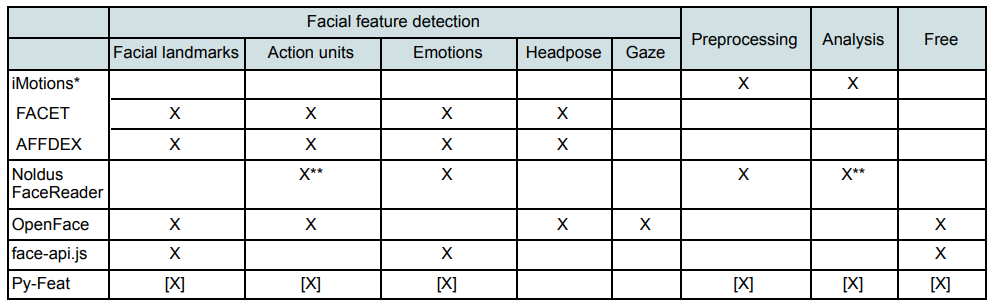
\includegraphics[width=5.5in]{example/faceExpression.png}
\caption{\begin{flushleft}\textbf{软件功能的比较以及是否收费:}X indicates features provided by each package. Features from Py-Feat toolbox are shown in brackets. Facial landmarks are points pertaining to locations of key spatial positions of the face including the jaw, mouth, nose, eyes, and eyebrows. Action units are facial muscle groups defined by FACS. Emotions refer to the detection of canonical emotional expressions. Headpose refers to the pitch, roll, and yaw orientations of the face. Gaze refers to the direction the eyes are looking. *iMotions is a platform and it’s feature extraction relies on the purchase of either the AFFDEX or FACET modules. **Detection of action units and analysis functionalities require a separate add-on purchase of The Action Unit Module and the Project Analysis Module for the Noldus FaceReader.\end{flushleft}}
\label{fig1:4-9}
\end{figure}

\begin{figure}[!htp]
\centering
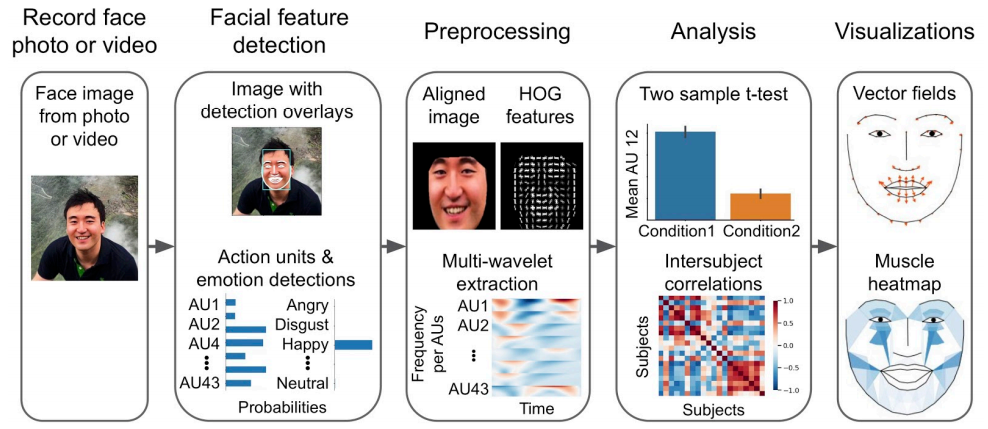
\includegraphics[width=5.5in]{example/faceExpression1.png}
\caption{\begin{flushleft}\textbf{人脸表情分析流水线:}Analysis of facial expressions begins with recording face photos or videos using a recording device such as webcams, camcorders, head mounted cameras, or 360 cameras. After capturing the face, researchers can use Py-Feat to detect facial features such as facial landmarks, action units, and emotions, and check the detection results with image overlays and bar graphs. The detection results can be preprocessed by extracting additional features such as Histogram of Oriented Gradients or multi-wavelet decomposition. Resulting data can then be analyzed within the toolbox using statistical methods such as t-tests, regressions, and intersubject correlations. Visualization functions can generate face images from models of action unit activations to show vector fields depicting landmark movements and heatmaps of facial muscle activations. \end{flushleft}}
\label{fig1:4-10}
\end{figure}

\subsubsection{Detectors模块}
1、Face Detectors

在Face Detectors模块中,Py-Feat使用Faceboxes(2018),MTCNN(2020),RetinaFace(2019)模型,并以WIDER FACE数据集为基准进行模型的训练,对于遮挡和非正脸的检测效果比较好。Py-Feat 默认使用RetinaFace进行人脸检测,如图\href{fig:4-11}{4-11} 所示。\\

\begin{figure}[!htp]
\centering
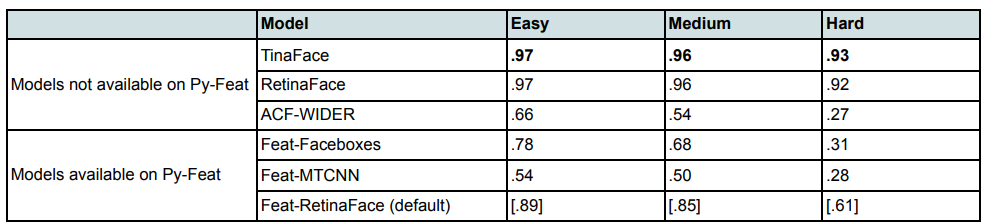
\includegraphics[width=5.5in]{example/faceExpression2.png}
\caption{\begin{flushleft}\textbf{以WIDER Face为基准的人脸边界框检测:} Easy, Medium, Hard results retrieved from WIDER Face. Numbers are average precision scores with higher numbers indicating better detection accuracy. Bold numbers indicate best performance for each column and bracketed numbers indicate the performance of the model selected as the default for Py-Feat. \end{flushleft}}
\label{fig1:4-11}
\end{figure}

2、Facial landmark detectors

在Facial landmark detectors模块中,Py-Feat使用Practical Facial Landmark Detector (PFLD,2019),MobileNets(2017)和MobileFaceNets(2018) 模型,并以300 Faces in the Wild (300W)数据集为基准进行模型的训练。Py-Feat默认使用MobileNet 进行人脸关键点检测,如图\href{fig:4-12}{4-12} 所示。\\

\begin{figure}[!htp]
\centering
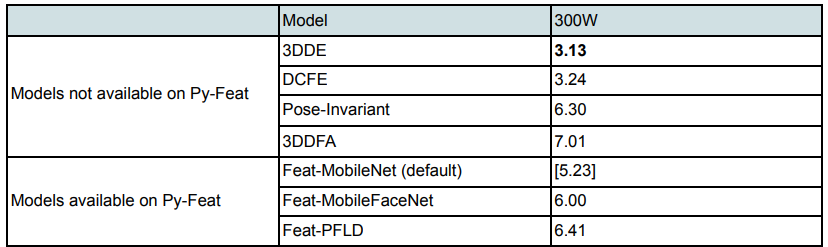
\includegraphics[width=5.5in]{example/faceExpression3.png}
\caption{\begin{flushleft}\textbf{以300W为基准的人脸关键点检测:}Feat models were initialized with face bounding boxes using RetinaFace. Numbers are root mean squared errors of coordinates with lower numbers indicating better alignment. Bold bracketed numbers indicate best performance for each column and bracketed numbers indicate the performance of the model selected as the default for Py-Feat. \end{flushleft}}
\label{fig1:4-12}
\end{figure}

3、Action unit detectors

在Action unit detectors模块中,Py-Feat使用了JAA-Net(2020)深度学习模型,以及RF,SVM和Logistic统计学习模型进行面部动作单元(AUs) 检测。

在端到端的JAA-Net模型中,以BP4D,BP4D+数据集为基准进行模型的训练,通过自适应注意力机制提取每个AUs的注意力图,去检测人脸关键点和AUs。

在统计学习模型中,RF,SVM和Logistic以BP4D,DISFA,CK+,Shoulder Pain,AFF-Wild2数据集为基准进行模型的训练,实现对AUs的检测。

Py-Feat只对12个AUs区域进行检测:AU1,AU2,AU4,AU5,AU6,AU9,AU12,AU15,AU17,AU20,AU25,和AU26,默认使用RF模型,如图\href{fig:4-13}{4-13} 所示。\\

\begin{figure}[!htp]
\centering
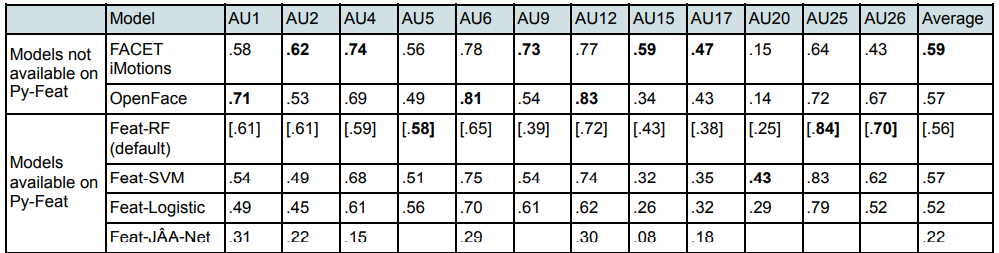
\includegraphics[width=5.5in]{example/faceExpression4.png}
\caption{\begin{flushleft}\textbf{以DisfaPlus为基准的人脸动作单元检测:}Numbers shown are F1 scores. Bold bracketed numbers indicate best performance for each column and bracketed numbers indicate the performance of the model selected as the default for Py-Feat. \end{flushleft}}
\label{fig1:4-13}
\end{figure}

4、Emotion detectors

在Emotion detectors模块中,Py-Feat使用ResMaskNet和FerNet深度学习模型,以及SVM,RF统计学习模型对7 种情感:anger,disgust,fear,happiness,sadness,surprise和neutral 进行识别。

对于ResMaskNet,使用FER数据集进行训练,对于FerNet,使用ExpW,CK+ 和JAFFE数据集进行训练。Py-Feat默认使用ResMaskNet进行表情识别,如图\href{fig:4-14}{4-14} 所示。

\begin{figure}[!htp]
\centering
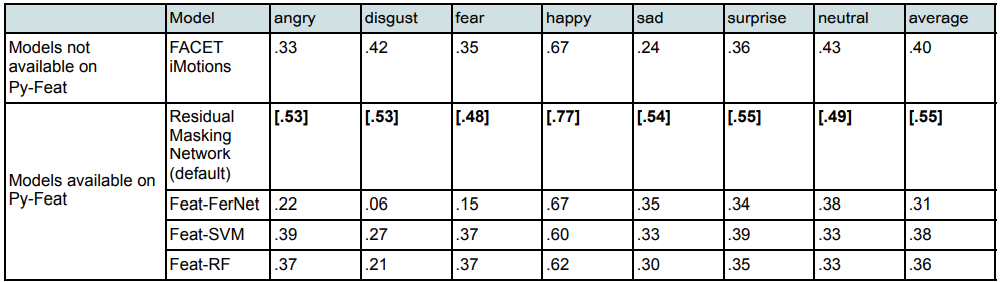
\includegraphics[width=5.5in]{example/faceExpression5.png}
\caption{\begin{flushleft}\textbf{以AffectNet为基准的人脸表情识别:} Numbers shown are F1 scores. Bold bracketed numbers indicate best performance for each column and bracketed numbers indicate the performance of the model selected as the default for Py-Feat.\end{flushleft}}
\label{fig1:4-8}
\end{figure}

\subsubsection{Fex数据处理模块}

Fex类是Pandas DataFrame的扩展,我们可以利用Pandas提供的切片、分组、取样功能对数据进行操作,也可以使用Fex类提供的专门函数来处理面部表情数据,这里的表情数据已经由Fex类封装好了( faceboxes,landmark,AU,Emotion)。Fex数据处理模块主要包括预处理模块,分析模块和可视化模块,如图\href{fig:4-10}{4-10} 所示。\\

1、预处理模块

因为不同人的相貌特征在先天上存在区别,因此不同人所表现的AU强度往往是不同的,比如有些人在无表情时略带微笑,有些人却略带皱眉。好的方法是通过初始化一个人的AU强度,确立人在无表情下AU强度的基线,减少不同人因不同样貌特征而存在的AU强度表现上的差异。

在对视频中人脸表情进行分析时,我们可以通过Emotion Detector识别每一帧中人的面部表情得分,进而得到在时间序列上的表情信号,接着通过常见的信号处理方法来处理:peak,最小值,平均值,频域分析等。\\

2、分析模块

Py-Feat提供一些基本的分析方法:t-test,回归,主体间相关性。\\

3、可视化模块

对于一张静态图片或者视频帧,Py-Feat提供了plot$\_$detection方法,对图片中人脸、人脸关键点、动作单元的检测结果和情绪识别的结果进行绘制。

\subsection{Aff-Wild2开源数据集}

1873年,Wilhelm Wundt设计了一个二维情感分类系统(情感轮),如图\href{fig:4-17}{4-17}所示。表情按照不同维度可如下划分:
\begin{enumerate}
\item 如果按照Valence(即愉悦程度)从Negative到Positive进行划分,害怕、生气、厌恶、伤心归为Negative(unpleasant),惊讶、开心、放松归为Positive (pleasant);
\item 如果按照Arousal(即情绪波动程度)从Passive到Active进行划分,厌恶、伤心、放松归为Passive(mild),惊讶、开心、害怕、生气归为Active(intense)。
\end{enumerate}

\begin{figure}
  \centering
  % Requires \usepackage{graphicx}
  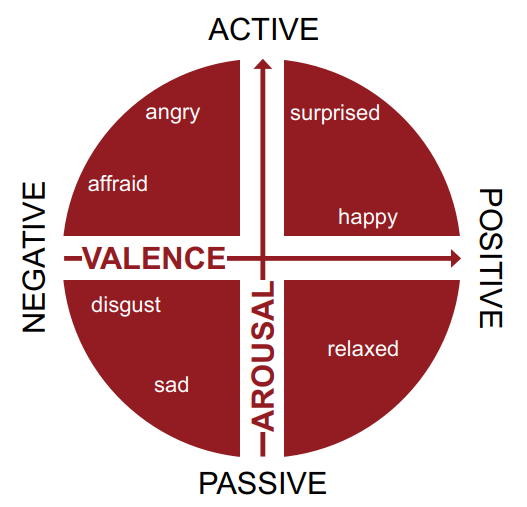
\includegraphics[width=2.5in]{figure/example/Aff-Wild3.png}\\
  \caption{The 2-D Emotion Wheel}
  \label{fig:4-17}
\end{figure}

\quad \\

\href{https://ibug.doc.ic.ac.uk/resources/aff-wild2/}{Aff-Wild2下载地址}

\href{https://www.sci-hub.ren/10.1109/CVPRW.2017.248}{Aff-Wild2论文地址}

Aff-Wild是第一个大型“野生”表情数据库,包含60多个小时的视频数据,基本上每帧视频都包含Valence-arousal标注,8种AU标注和7种情绪标注,可以进行多任务学习。如图\href{fig:4-18}{4-18}所示\footnote{A Multi-Task Learning & Generation Framework: Valence-Arousal,
Action Units & Primary Expressions \quad \url{https://arxiv.org/abs/1811.07771}}。

\begin{figure}
  \centering
  % Requires \usepackage{graphicx}
  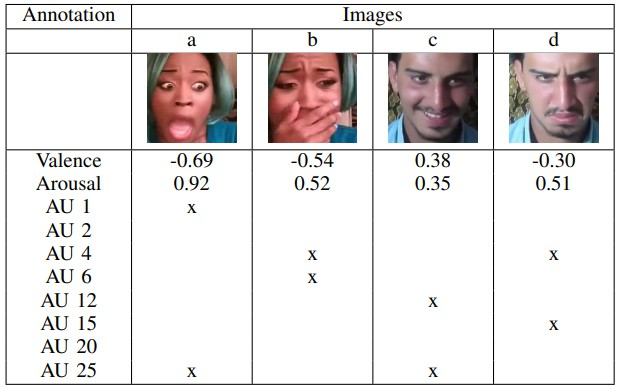
\includegraphics[width=4in]{figure/example/Aff-Wild1.jpg}\\
  \caption{Images with their corresponding VA and AU annotations}
  \label{fig:4-18}
\end{figure}

\quad \\

1、VA Set

每个标注文件均以其对应的视频命名,第一行始终是:valence,arousal,而第一行之后的每一行均显示用逗号分隔的valence和arousal值,valence和arousal的取值范围为$[-1,1]$。若存在值为$(-5,-5)$,则表示此帧未使用valence,arousal进行标注,需要忽略此帧。

\quad \\

2、AU Set

在Aff-Wild中共64个视频,其中至少包含一种AU的帧数为139298帧,未标注AU的帧数为40702帧,总帧数为180000帧。 每个标注文件均以其对应的视频命名,每个标注文件的第一行始终为:AU1,AU2,AU4,AU6,AU12,AU15,AU20,AU25。第一行之后的每一行均显示AU注释值,以逗号分隔,每个值可以是0或1或-1,标有-1的帧表示该帧未标注AU,应被丢弃。Aff-Wild中的AU统计量如图\href{fig:4-19}{4-19}所示。
\begin{figure}
  \centering
  % Requires \usepackage{graphicx}
  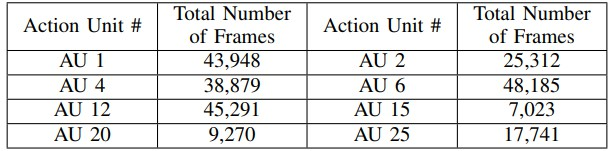
\includegraphics[width=4in]{figure/example/Aff-Wild2.jpg}\\
  \caption{Total number of frames with a specific AU}
  \label{fig:4-19}
\end{figure}

\quad \\

3、Expression Set

每个标注文件均以其对应的视频命名,第一行始终为:netural,anger,disgust,fair,happy,sadness,suprised。第一行之后的每一行用{0,1,2,3,4,5,6}某个值进行标注,这些值分别对应于不同的情绪。 如果标注值为-1,表示该帧未标注情绪,应被丢弃。Aff-Wild中存在一些视频,这些视频中包含两个主题,对应受试者所看到的不同的内容。两个主题都有标注,并且相应的标注文件以结尾扩展名$\_left$和$\_right$进行了区分。

\section{人脸姿态估计}

姿态估计问题是确定某一三维目标物体的方位指向问题,姿态估计在机器人视觉、动作跟踪和单照相机定标等很多领域都有应用。在不同领域用于姿态估计的传感器(单目摄像头,双目摄像头,激光雷达)是不一样的。显然,人脸姿态估计是属于其中的范畴。

在日常交流中,我们不仅可以通过对方说话的内容,语音和语调,也可以通过对方的肢体语言去理解一个人的性格或者内心小情绪。对于肢体语言,一般是指通过头、眼、颈、手、肘、臂、身、胯、足等人体部位的协调活动来传达人物的思想,形象地借以表情达意的一种沟通方式。在我看来,人脸姿态估计相对于人脸表情识别来说,是一种更加宏观,客观的识别方式,主要包括对头部运动的估计,和对眼动的追踪。接下来我主要介绍人脸姿态估计中的头部运动估计。

通过头部运动方向,我们可以分析一个人此时注意力是否集中,对某样东西是否感兴趣?头部姿态估计的应用场景主要包括:社交行为分析,司机辅助系统和人机交互。

头部姿势运动有三个自由度x,y,z,对于不同坐标轴的旋转又可分成yaw, pitch 和roll。在三维空间的右手笛卡尔坐标中,yaw,pitch和poll如图\href{fig:4-9}{4-9}所示;在航空中(使用右手笛卡尔坐标系),pitch 是围绕X轴旋转,也叫做俯仰角,yaw是围绕Y轴旋转,也叫偏航角,roll 是围绕Z轴旋转,也叫翻滚角,如图\href{fig:4-10}{4-10} 所示。

\begin{figure}[!htp]
\centering
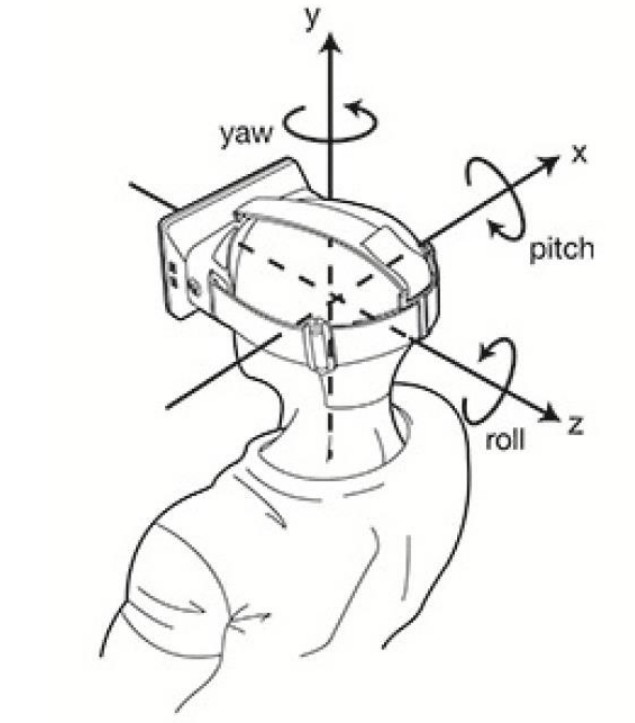
\includegraphics[width=3in]{example/PnP2.jpg}
\caption{右手笛卡尔坐标系中的yaw, pitch和roll}
\label{fig1:4-8}
\end{figure}

\begin{figure}[!htp]
\centering
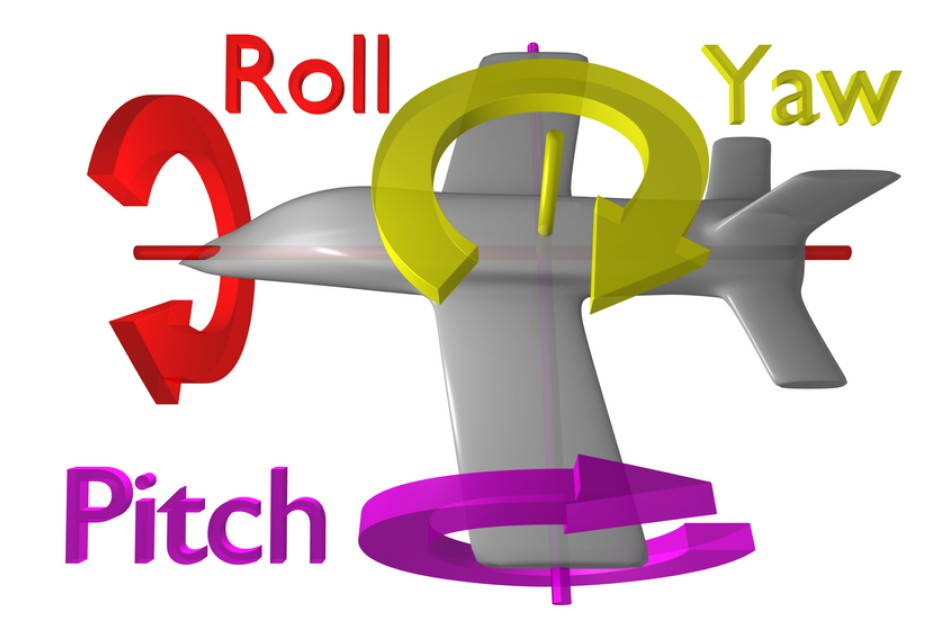
\includegraphics[width=3in]{example/PnP3.jpg}
\caption{飞行器中的yaw, pitch和roll}
\label{fig1:4-8}
\end{figure}

了解了什么是人脸姿态估计之后,接下来我们来理解一下姿态估计中的PnP问题。

\subsection{什么是PnP问题}

在3D视觉中,我们可以通过移动对象的位置、移动相机的位置或者调节相机的内参数来修改相机最终输出图像中对象的姿态。我们接下来描述的人脸姿态估计问题通常在3D计算机视觉中称为n 点透视问题或PnP(Perspective-n-Point) 问题,其中n表示3D-2D点对的个数。对PnP 问题的求解,即对三维空间点到二维空间点映射关系的求解(通俗来讲,就是求解三维到二维空间的变换矩阵),它可以用来估计相机所在的位姿,或者物体的位姿(这二者是等价的),PnP问题的直观描述如图\href{fig:4-6}{4-6}所示。
\footnote{3D-2D:PnP算法原理 \quad \url{https://blog.csdn.net/u014709760/article/details/88029841}}。

\begin{figure}[!htp]

\centering
%\begin{minipage}[t]{5in}
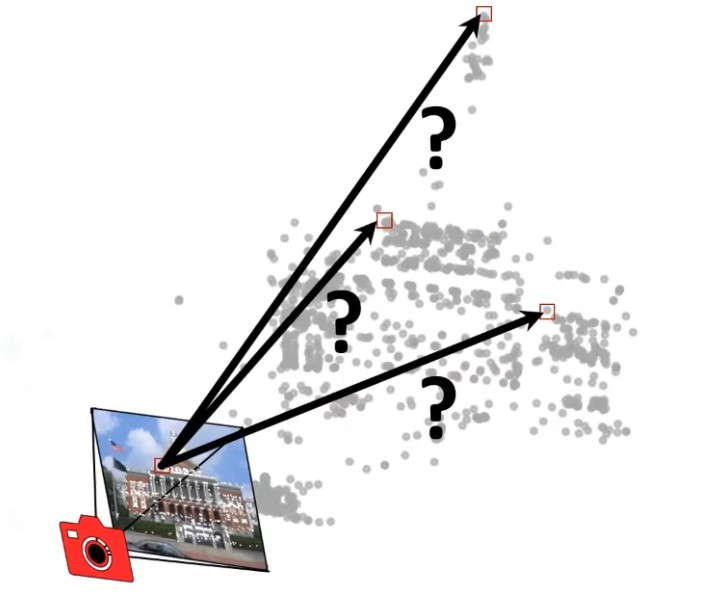
\includegraphics[width=4in]{example/PnP.jpg}
\caption{PnP问题}
\label{figure:4-6}
%\end{minipage}
\end{figure}

PnP问题有很多种求解方法,例如用三对人脸关键点估计位姿的P3P方法 、直接线性变换(DLT)、EPnP方法等。此外,还能用非线性优化的方式,构建最小二乘问题并迭代求解。

这里要注意的是,PnP问题的求解方法实际上只是姿态估计中的一类方法,一般是在给定某物体在三维空间(世界坐标系)上点的坐标,以及二维空间(图像坐标系)上点的坐标的情况下,寻找表示两个空间上点一一映射关系的变换矩阵。对于其他的姿态估计方法,可以先不给定2D-3D 关键点的对应关系,而是通过同时输入同个物体的3D和2D的特征,使用神经网络学习其对应关系(这种方法可以称为blind PnP)。

\subsection{相机成像原理}

\subsubsection{针孔模型}

数码相机图像拍摄的过程实际上是一个光学成像的过程。相机的成像过程涉及到四个坐标系:世界坐标系、相机坐标系、图像坐标系、像素坐标系以及这四个坐标系的转换。

相机模型是光学成像模型的简化,目前有线性模型和非线性模型两种。实际的成像系统是透镜成像的非线性模型。最基本的透镜成像原理如图\href{fig:4-11}{4-11}所示\footnote{针孔成像模型讲解 \quad \url{https://blog.csdn.net/a1059682127/article/details/80632168}}。

\begin{figure}[!htp]
\centering
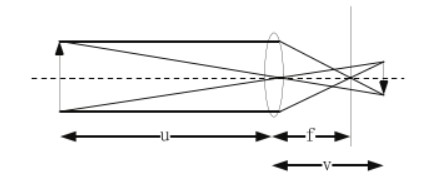
\includegraphics[width=3in]{example/Camera1.jpg}
\caption{透视成像原理示意图}
\label{fig1:4-11}
\end{figure}

其中u为物距,f为焦距,v为像距。三者满足关系式

\begin{align}
& \frac{1}{f} = \frac{1}{u} + \frac{1}{v}
\end{align}

相机的镜头是一组透镜,当平行于主光轴的光线穿过透镜时,会聚到一点上,这个点叫做焦点,焦点到透镜中心的距离叫做焦距f。数码相机的镜头相当于一个凸透镜,感光元件就处在这个凸透镜的焦点附近,将焦距近似为凸透镜中心到感光元件的距离时就成为小孔成像模型。小孔成像模型如图\href{fig:4-12}{4-12}所示。

\begin{figure}[!htp]
\centering
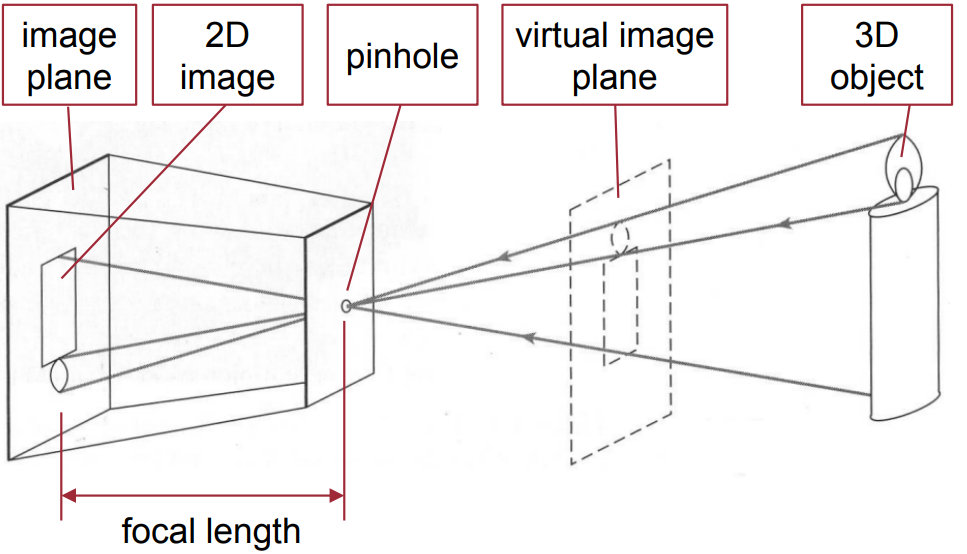
\includegraphics[width=3in]{example/Camera2.jpg}
\caption{小孔成像模型}
\label{fig1:4-11}
\end{figure}

小孔成像模型是相机成像采用最多的模型。在此模型下,物体的空间坐标和图像坐标之间是线性的关系,因而对相机参数的求解就归结到求解线性方程组上。四个坐标系的关系图如图\href{fig:4-13}{4-13} 所示,其中 M 为三维空间点,m 为 M 在图像平面投影成的像点。
\begin{figure}[!htp]
\centering
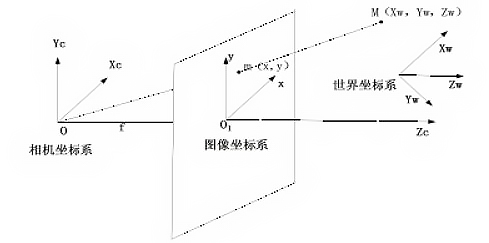
\includegraphics[width=3in]{example/Camera3.jpg}
\caption{四个坐标关系示意图}
\label{fig1:4-11}
\end{figure}

①世界坐标系:是客观三维世界的绝对坐标系,也称客观坐标系。因为数码相机安放在三维空间中,我们需要世界坐标系这个基准坐标系来描述数码相机的位置,并且用它来描述安放在此三维环境中的其它任何物体的位置,用$(X_w,Y_w,Z_w)$表示其坐标值。

②相机坐标系(光心坐标系):以相机的光心为坐标原点,X 轴和Y 轴分别平行于图像坐标系的 X 轴和Y轴,相机的光轴为Z轴,用$(X_c,Y_c,Z_c)$表示其坐标值。

③图像坐标系:以CCD 图像平面的中心为坐标原点,X轴和Y 轴分别平行于图像平面的两条垂直边,用$(x,y)$表示其坐标值。图像坐标系是用物理单位(例如毫米)表示像素在图像中的位置。

④像素坐标系:以 CCD 图像平面的左上角顶点为原点,X 轴和Y 轴分别平行于图像坐标系的 X 轴和Y 轴,用$(u,v)$表示其坐标值。数码相机采集的图像首先是形成标准电信号的形式,然后再通过模数转换变换为数字图像。每幅图像的存储形式是M $\times$ N的数组,M 行 N 列的图像中的每一个元素的数值代表的是图像点的灰度。这样的每个元素叫像素,像素坐标系就是以像素为单位的图像坐标系。

\subsubsection{实际成像模型}

理想的透视模型是针孔成像模型,物和像会满足相似三角形的关系。但是实际上由于相机光学系统存在加工和装配的误差,透镜就并不能满足物和像成相似三角形的关系,所以相机图像平面上实际所成的像与理想成像之间会存在畸变。畸变属于成像的几何失真,是由于焦平面上不同区域对图像的放大率不同形成的画面扭曲变形的现象,这种变形的程度从画面中心至画面边缘依次递增,主要在画面边缘反映比较明显。为了减小畸变,拍摄图片时应尽量避免用镜头焦距的最广角端或最远端拍摄。实际的相机成像模型如图\href{fig:4-12}{4-12} 所示\footnote{针孔成像模型讲解 \quad \url{https://blog.csdn.net/a1059682127/article/details/80632168}}。
\begin{figure}[!htp]
\centering
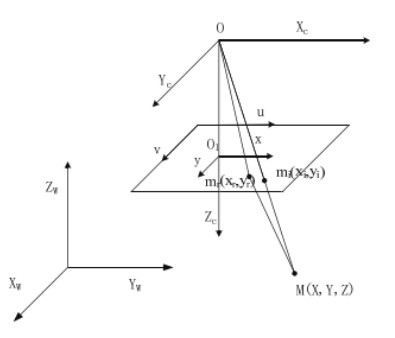
\includegraphics[width=2.5in]{example/Camera5.jpg}
\caption{实际相机模型}
\label{fig1:4-12}
\end{figure}

\subsection{旋转的表示方式}

3D物体相对相机(即世界坐标系的物体相对于相机坐标系的"物体")来说只存在两种运动\footnote{使用opencv和dlib进行人脸姿态估计(python) \quad \url{https://blog.csdn.net/yuanlulu/article/details/82763170}}
\footnote{Head Pose Estimation using OpenCV and Dlib \quad \url{https://learnopencv.com/head-pose-estimation-using-opencv-and-dlib/}},一种是平移,一种是旋转。

1、平移:将相机从当前的3D位置$(X,Y,Z)$移动到新的3D位置$(X',Y',Z')$称为平移,物体可以在3个自由度(x,y,z方向)上移动,用向量$t = (X'-X,Y'-Y,Z'-Z)$表示。

2、旋转:相比于平移,旋转也具有三个自由度x,y,z。如果对某个刚体在三维空间进行任意次的旋转,只要旋转中心保持不变,无论多少次的旋转都可以用绕三维空间中某一个轴的一次旋转来表示。表示三维空间的旋转有多种互相等价的方式,常见的有旋转矩阵(Rotation Matrix)、 方向余弦矩阵(Direction Cosine Matrix)、旋转向量(Rotation Vector)、四元数(Quaternion)、 方向余弦矩阵(Direction Cosine Matrix)、欧拉角(Euler angle) 等。我们需要了解一下这些旋转表示方式以及它们之间的相互转换方式
\footnote{刚体在三维空间的旋转 \quad \url{https://blog.csdn.net/yuewei19/article/details/53023992}}。

\subsubsection{旋转矩阵(3 $\times$  3)}

1、基本旋转矩阵\footnote{Rotation matrix \quad \url{https://en.wikipedia.org/wiki/Rotation_matrix#Examples}}:

基本旋转是指围绕坐标系中某一个轴进行的旋转,以下三个基本旋转矩阵是在三维空间中用右手法则将向量分别绕$x$、$y$、$z$ 轴旋转一个θ 角得到的,右手法则将它们的交替符号表示出来。
\begin{align}
&{\displaystyle {\begin{alignedat}{1}R_{x}(\theta )&={\begin{bmatrix}1&0&0\\0&\cos \theta &-\sin \theta \\[3pt]0&\sin \theta &\cos \theta \\[3pt]\end{bmatrix}}\\[6pt]R_{y}(\theta )&={\begin{bmatrix}\cos \theta &0&\sin \theta \\[3pt]0&1&0\\[3pt]-\sin \theta &0&\cos \theta \\\end{bmatrix}}\\[6pt]R_{z}(\theta )&={\begin{bmatrix}\cos \theta &-\sin \theta &0\\[3pt]\sin \theta &\cos \theta &0\\[3pt]0&0&1\\\end{bmatrix}}\end{alignedat}}}
\end{align}

假设坐标系使用右手坐标系、角$\theta$为正,对于向量,当它们所绕的轴指向观察者时,这些基本的矢量旋转都是逆时针的。例如,对于$x$ 轴上的向量$(1,0,0)$,通过$R_z(90^{\circ })$ 可将其旋转到$y$轴,得到向量$(0,1,0)$。

\begin{align}
& {\displaystyle R_{z}(90^{\circ }){\begin{bmatrix}1\\0\\0\\\end{bmatrix}}={\begin{bmatrix}\cos 90^{\circ }&-\sin 90^{\circ }&0\\\sin 90^{\circ }&\quad \cos 90^{\circ }&0\\0&0&1\\\end{bmatrix}}{\begin{bmatrix}1\\0\\0\\\end{bmatrix}}={\begin{bmatrix}0&-1&0\\1&0&0\\0&0&1\\\end{bmatrix}}{\begin{bmatrix}1\\0\\0\\\end{bmatrix}}={\begin{bmatrix}0\\1\\0\\\end{bmatrix}}}
\end{align}

\quad \\

2、一般旋转矩阵:

通过对下面这三个矩阵做矩阵乘法,我们可以得到一般旋转矩阵:
\begin{align}
& {\displaystyle R=R_{z}(\alpha )\,R_{y}(\beta )\,R_{x}(\gamma )={\overset {\text{roll}}{\begin{bmatrix}\cos \alpha &-\sin \alpha &0\\\sin \alpha &\cos \alpha &0\\0&0&1\\\end{bmatrix}}}{\overset {\text{yaw}}{\begin{bmatrix}\cos \beta &0&\sin \beta \\0&1&0\\-\sin \beta &0&\cos \beta \\\end{bmatrix}}}{\overset {\text{pitch}}{\begin{bmatrix}1&0&0\\0&\cos \gamma &-\sin \gamma \\0&\sin \gamma &\cos \gamma \\\end{bmatrix}}}} \\
& {\displaystyle R={\begin{bmatrix}\cos \alpha \cos \beta &\cos \alpha \sin \beta \sin \gamma -\sin \alpha \cos \gamma &\cos \alpha \sin \beta \cos \gamma +\sin \alpha \sin \gamma \\\sin \alpha \cos \beta &\sin \alpha \sin \beta \sin \gamma +\cos \alpha \cos \gamma &\sin \alpha \sin \beta \cos \gamma -\cos \alpha \sin \gamma \\-\sin \beta &\cos \beta \sin \gamma &\cos \beta \cos \gamma \\\end{bmatrix}}}
\end{align}

其中$R$是个旋转矩阵,其偏航角(yaw),俯仰角(pitch)和侧倾角(roll) 分别为$\alpha$,$\beta$和$\gamma$,更准确来说,R绕轴$z,y,x$ 的欧拉角分别为$\alpha$,$\beta$和$\gamma$。因为在一般情况下矩阵乘法是不可交换的,因此只有当这些矩阵以指定的顺序相乘时,这些矩阵才会产生所需的旋转效果。

因为平移和旋转都具有3个自由度,因此对于3D对象的姿态估计,我们需要用6 个变量(3个用于平移,3个用于旋转)来描述对象的姿态。

\subsubsection{欧拉角}

最直观的表示方式是绕刚体自身的X、Y、Z三个轴分别进行旋转某个角度,这就是所谓的欧拉角(Euler Angle)表示方式\footnote{Euler angles \quad \url{https://en.wikipedia.org/wiki/Euler_angles}} \footnote{刚体在三维空间的旋转 \quad \url{https://blog.csdn.net/yuewei19/article/details/53023992}}。

需要注意的是,在欧拉角的表示方式里,yaw、pitch、roll的顺序对旋转的结果是有影响的。给定一组欧拉角角度值,比如yaw=45度,pitch=30 度,roll=60度,按照yaw-pitch-roll 的顺序旋转和按照yaw-roll-pitch 的顺序旋转,最终刚体的朝向是不同的!换言之,若刚体需要按照两种不同的旋转顺序旋转到相同的朝向,所需要的欧拉角角度值则是不同的!如果魔方的核看做是一个刚体的话,拧魔方这个例子能较好地解释因绕轴旋转顺序的不同,最终刚体的朝向也不同。

另外需要注意的是,在欧拉角的表示方式里,三个旋转轴一般是随着刚体在运动,即wikipedia中所谓的intrinsic rotation。相对应的另一种表示方式是,三个旋转轴是固定的,不随刚体旋转而旋转,即extrinsic rotation,这种表示方式在计算机视觉中不是很常用。

欧拉角的表示方式比较直观,但是有几个缺点:

①欧拉角的表示方式不唯一。给定某个起始朝向和目标朝向,即使给定yaw、pitch、roll的顺序,也可以通过不同的yaw/pitch/roll的角度组合来表示所需的旋转。比如,同样的yaw-pitch-roll顺序,$(0,90,0)$ 和$(90,90,90)$会将刚体转到相同的位置。这其实主要是由于万向锁(Gimbal Lock)引起的,关于万向锁的解释,有条件的同学看看Youtube 的视频或许会比较直观。

② 欧拉角的插值比较难。

③ 计算旋转变换时,一般需要转换成旋转矩阵,这时候需要计算很多sin, cos,计算量较大。

\subsubsection{方向余弦矩阵}

方向余弦矩阵(Direction Cosine Matrix)其实是旋转矩阵的另一个叫法,简称DCM,在陀螺力学领域较为常用。DCM的名字来历其实是用欧拉角之外的另一种用3个角度值表示三维旋转的方式,假设刚体在起始朝向时三个坐标轴的向量为I,J,K,而刚体在目标朝向时的三个坐标轴的向量为i,j,k,则该旋转可以通过三个坐标轴分别与原始坐标轴的夹角表示,如图
\href{fig:4-13}{4-13}所示

\begin{figure}[!htp]
\centering
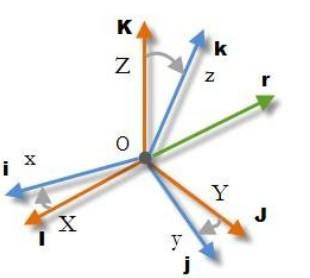
\includegraphics[width=2.5in]{example/DCM.jpg}
\caption{方向余弦矩阵DCM}
\label{fig1:4-13}
\end{figure}

DCM可以通过三个夹角的余弦计算如下:
\begin{align}
\begin{bmatrix}
i^G & j^G & k^G
\end{bmatrix}
=
\begin{bmatrix}
cos(I,i) & cos(I,j) & cos(I,k) \\
cos(J,i) & cos(J,j) & cos(J,k) \\
cos(K,i) & cos(K,j) & cos(K,k)
\end{bmatrix}
=
DCM^G
\end{align}

\subsection{相机的内参数,外参数}

在图像测量过程以及机器视觉应用中,为确定空间物体表面某点的三维几何位置与其在图像中对应点之间的相互关系,必须建立相机成像的几何模型,这些几何模型参数就是相机参数。在大多数条件下这些参数必须通过实验与计算才能得到,这个求解参数的过程就称之为相机标定(或摄像机标定)\footnote{计算机视觉-相机内参数和外参数 \quad \url{https://baijiahao.baidu.com/s?id=1603212014194819932&wfr=spider&for=pc}}。

相机标定的目的是确定相机的一些参数的值。通常,这些参数可以建立定标板确定的三维坐标系和相机图像坐标系的映射关系,换句话说,你可以用这些参数把一个三维空间中的点映射到图像空间,或者反过来。

相机参数主要包括相机内参数和相机的外参数。相机内参数是与相机自身特性相关的参数,比如相机的焦距、像素大小等;相机外参数是在世界坐标系中的参数,比如相机的位置、旋转方向等。有了这些参数,我们可以实现不同坐标系的相互转换。

前面已经介绍了关于相机的4种坐标系,接下来将依次介绍世界坐标系$(X_w,Y_w,Z_w)$,相机坐标系$(X_c,Y_c,Z_c)$,图像坐标系$(x,y)$ 和像素坐标系$(u,v)$的转换关系。

1、像素坐标系与图像坐标系的转换:

像素坐标系与图像坐标系关系如图\href{fig:4-12}{4-12}所示,之间的转换关系为:

\begin{align}
& u = \frac{x}{dx} + u_0  \\
& v = \frac{y}{dy} + v_0
\end{align}

\begin{figure}[!htp]
\centering
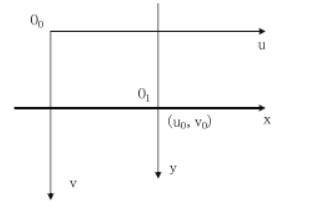
\includegraphics[width=2in]{example/Camera4.jpg}
\caption{像素坐标系与图像坐标系关系图}
\label{fig1:4-12}
\end{figure}

采用齐次坐标再用矩阵形式将上式表示为:
\begin{align}
\begin{pmatrix}
u \\ v \\ 1
\end{pmatrix}
=
\begin{pmatrix}
\frac{1}{dx} & 0 & u_0 \\
0 & \frac{1}{dy} & v_0 \\
0 & 0 & 1
\end{pmatrix}
\begin{pmatrix}
x \\ y \\ 1
\end{pmatrix}
\end{align}

其中$(u_0, v_0)$是图像坐标系原点在像素坐标系中的坐标,$dx$和$dy$ 分别是每个像素在图像平面x和y方向上的物理尺寸。

2、图像坐标系与相机坐标系的转换:

\begin{align}
& x = \frac{fX_c}{Z_c}  \\
& y = \frac{fY_c}{Z_c}
\end{align}

其中 f 为焦距(像平面与相机坐标系原点的距离)。用齐次坐标系和矩阵表示上述关系:
\begin{align}
Z_c\begin{pmatrix}
x \\ y \\ 1
\end{pmatrix}
=
\begin{pmatrix}
f & 0 & 0 & 0\\
0 & f & 0 & 0\\
0 & 0 & 1 & 0
\end{pmatrix}
\begin{pmatrix}
X_c \\ Y_c \\ Z_c \\ 1
\end{pmatrix}
\end{align}

3、相机坐标系与世界坐标系的转换:

\begin{align}
\begin{pmatrix}
X_c \\ Y_c \\ Z_c \\ 1
\end{pmatrix}
=
\begin{pmatrix}
R & t \\
0^T & 1
\end{pmatrix}
\begin{pmatrix}
X_w \\ Y_w \\ Z_w \\ 1
\end{pmatrix}
\end{align}

其中 R 为3 $\times$ 3正交旋转矩阵,t 为三维平移向量

4、像素坐标系与世界坐标系的变换:
\begin{align}
&Z_c\begin{pmatrix}
u \\ v \\ 1
\end{pmatrix}
=
Z_c\begin{pmatrix}
\frac{1}{dx} & 0 & u_0 \\
0 & \frac{1}{dy} & v_0 \\
0 & 0 & 1
\end{pmatrix}\begin{pmatrix}
x \\ y \\ 1
\end{pmatrix} \\
& =
\begin{pmatrix}
\frac{1}{dx} & 0 & u_0 \\
0 & \frac{1}{dy} & v_0 \\
0 & 0 & 1
\end{pmatrix}\begin{pmatrix}
f & 0 & 0 & 0\\
0 & f & 0 & 0\\
0 & 0 & 1 & 0
\end{pmatrix}
\begin{pmatrix}
R & t \\
0^T & 1
\end{pmatrix}
\begin{pmatrix}
X_w \\ Y_w \\ Z_w \\ 1
\end{pmatrix} \\
& =
\begin{pmatrix}
a_x & 0 & u_0 & 0\\
0 & a_y & v_0 & 0\\
0 & 0 & 1 & 0
\end{pmatrix}\begin{pmatrix}
R & t \\
0^T & 1
\end{pmatrix}
\begin{pmatrix}
X_w \\ Y_w \\ Z_w \\ 1
\end{pmatrix} \\
& =
KM_1\begin{pmatrix}
X_w \\ Y_w \\ Z_w \\ 1
\end{pmatrix} = M\begin{pmatrix}
X_w \\ Y_w \\ Z_w \\ 1\end{pmatrix}
= \begin{pmatrix}
m_{11} & m_{12} & m_{13} & m_{14}\\
m_{21} & m_{22} & m_{23} & m_{24}\\
m_{31} & m_{32} & m_{33} & m_{34}
\end{pmatrix}
\begin{pmatrix}
X_w \\ Y_w \\ Z_w \\ 1
\end{pmatrix}
\end{align}

其中:
\begin{align}
&a_x = \frac{f}{dx} \nonumber \\
&a_y = \frac{f}{dy} \nonumber \\
&K = \begin{pmatrix}
a_x & 0 & u_0 & 0 \\
0 & a_y & v_0 & 0 \\
0 & 0 & 1 & 0
\end{pmatrix} \nonumber \\
&M_1 = \begin{pmatrix}
R & t \\
0^T & 1
\end{pmatrix} \nonumber
\end{align}

$a_x$, $a_y$分别是图像水平轴和垂直轴的尺度因子。K的参数中只包含焦距、主点坐标等只由相机的内部结构决定,因此称 K 为内部参数矩阵,$a_x$, $a_y$ , $u_0$, $v_0$叫做内部参数。

$M_1$中包含的旋转矩阵和平移向量是由相机坐标系相对于世界坐标系的位置决定的,因此称$M_1$为相机的外部参数矩阵,R和t叫做外部参数,M 叫投影矩阵。相机标定就是确定相机的内部参数和外部参数。

\subsubsection{径向,切向畸变}

理想的透视模型是针孔成像模型,物和像会满足相似三角形的关系。但是真实的镜头还会有径向和切向畸变,透镜并不能满足物和像成相似三角形的关系,所以相机图像平面上实际所成的像与理想成像之间会存在畸变。畸变矩阵告诉你为什么上面那个像素点并没有落在理论计算该落在的位置上,而是产生了一定的偏移和变形(畸变属于相机的内参)。

\subsection{人脸姿态估计需要哪些信息}

如果要计算图像中目标对象的3D姿态,我们需要以下这些信息(如图\href{fig:4-15}{4-15}所示)\footnote{Head Pose Estimation using OpenCV and Dlib \quad \url{https://learnopencv.com/head-pose-estimation-using-opencv-and-dlib/}}:

\begin{figure}[!htp]
\centering
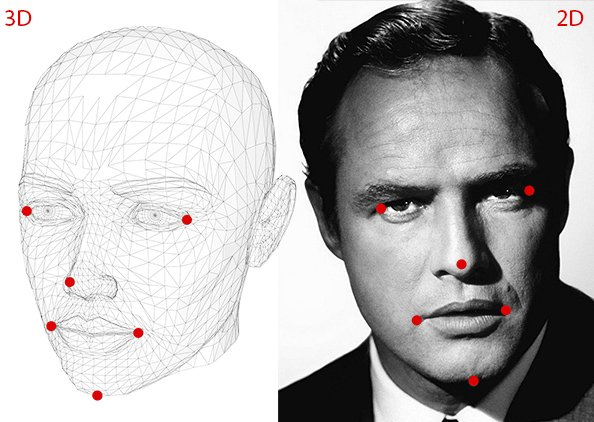
\includegraphics[width=3.5in]{example/3DPose1.jpg}
\caption{眼睛,鼻尖,嘴角等关键点}
\label{fig1:4-15}
\end{figure}

1、在图像坐标系下的人脸特征点(2D坐标):对于脸部的特征点,我们可以选择眼角,鼻尖,嘴角等对称部位。这里我们选择鼻尖,下巴,左眼角,右眼角,左嘴角和右嘴角的位置信息。

2、在世界坐标系下,人脸2D特征点对应的3D特征点坐标:对于3D特征点,其实我们无需通过照片中头部的3D模型来获取其位置信息,我们只需要在某个参考系中得到这些2D点的3D位置即可,这里我们可以定义以下点的3D坐标:

1)鼻尖:$(0.0,0.0,0.0)$

2)下巴:$(0.0,-330.0,-65.0)$

3)左眼左角:$(-225.0f,170.0f,-135.0)$

4)右眼右角:$(225.0,170.0,-135.0)$

5)嘴角左侧:$(-150.0,-150.0,-125.0)$

6)嘴角右侧:$(150.0,-150.0,-125.0)$

3、相机的内参数:我们需要知道相机的焦距,相机的光学中心和径向失真参数。通过不使用准确的3D模型,仅仅通过图像我们可以近似确定人脸在实际情况下的位置信息。我们可以通过图像的中心来逼近相机的光学中心,将焦距近似为图像的宽度,并假设不存在径向失真问题。因此在进行2D到3D转换过程中,内参数矩阵是通过图像本身的信息来近似的。

\subsection{姿态估计算法}

如图\href{fig:4-8}{4-8}所示图中有三个坐标系,在世界坐标系中包含面部特征的3D位置信息,如果我们知道旋转和平移(相机的外参数),我们可以将世界坐标系中的3D点变换到相机坐标中的3D点。如果我们知道相机的内参数(焦距,光学中心等),我们可以将相机坐标中的3D 点投影到图像平面(即图像坐标系)上。图中$o$是相机的光学中心,所示的平面是图像平面,我们的目标是找出某个方程,使得这个方程可以将3D 点$P$投影到图像平面的$p$点上。

\begin{figure}[!htp]
\centering
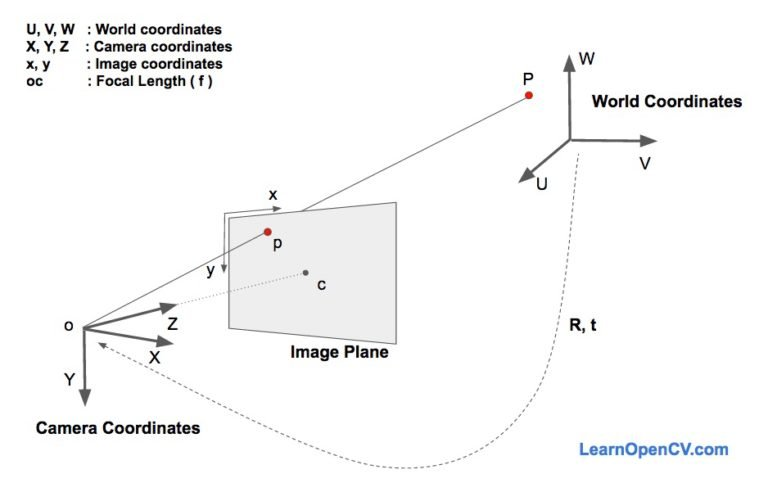
\includegraphics[width=4.5in]{example/3DPose.jpg}
\caption{世界、相机、图像坐标系的转换}
\label{fig1:4-8}
\end{figure}


假设我们知道世界坐标系中3D点$P$的位置$(U,V,W)$,知道旋转矩阵R (3 $\times$ 3矩阵)和平移向量t(3 $\times$ 1向量),我们可以使用以下公式计算摄像机坐标系中$P$点的位置$(X,Y,Z)$。
\begin{align}
&\begin{bmatrix} X \\ Y \\ Z \\ \end{bmatrix}
= R\begin{bmatrix} U \\ V \\ W \\ \end{bmatrix} +t \nonumber \\
&\Rightarrow \begin{bmatrix} X \\ Y\\ Z \\ \end{bmatrix}
= [R|t]\begin{bmatrix} U \\ V \\ W \\ 1 \\ \end{bmatrix}
\end{align}

上述方程可以具体写成如下形式
\begin{align}
&\begin{bmatrix}
X \\ Y \\ Z
\end{bmatrix}
= \begin{bmatrix}
r_{00} & r_{01} & r_{02} & t_x\\
r_{10} & r_{11} & r_{12} & t_y\\
r_{20} & r_{21} & r_{22} & t_z\\
\end{bmatrix}
\begin{bmatrix}
U \\ V \\ W \\ 1
\end{bmatrix}
\end{align}

如果我们知道足够数量点的对应关系(即$(X,Y,Z)$和$(U,V,W)$的对应关系),对于$r_{ij}$和$(t_x,t_y,t_z)$的未知数,我们可以通过上面的线性方程组求解,进而求解出变换矩阵$[R|t]$。\\

\subsubsection{直接线性变换}

我们知道3D模型上的许多点(即$(U,V,W)$),但是我们不知道$(X,Y,Z)$,只知道2D点的位置(即$(x,y)$)。在没有径向变形的情况下,图像坐标中点$p$的坐标$(x,y)$由下式给出
\begin{align}
& \begin{bmatrix}
x \\ y \\ 1
\end{bmatrix}
= s \begin{bmatrix}
f_x & 0 & c_x \\ 0 & f_y & c_y \\0 & 0 & 1
\end{bmatrix}
\begin{bmatrix}
X \\ Y \\ Z
\end{bmatrix}
\end{align}

其中,$f_x$和$f_y$是$x$和$y$方向上的焦距,$(c_x,c_y)$是光学中心。当涉及径向扭曲时,事情变得复杂得多,为了简单起见,这里不考虑径向扭曲。

方程中的$s$是一个未知的比例因子,它存在于等式中,因为在任何图像中我们并不知道图像的深度,需要$s$来调节。如果将3D中的任何点$P$ 连接到相机的中心$o$,则光线与图像平面相交的点$p$是$P$的图像。使用上述等式,我们只能计算出在刻度s下的坐标$(X,Y,Z)$。

通过上式可以看出,比例因子$s$影响了相机坐标系上$(X,Y,Z)$的取值,使得第二个方程不再是一个简单的线性方程了。
\begin{align}
s\begin{bmatrix}
X \\ Y \\ Z
\end{bmatrix}
= = \begin{bmatrix}
r_{00} & r_{01} & r_{02} & t_x\\
r_{10} & r_{11} & r_{12} & t_y\\
r_{20} & r_{21} & r_{22} & t_z\\
\end{bmatrix}
\begin{bmatrix}
U\\ V \\ W \\ 1
\end{bmatrix}
\end{align}

然而我们可以使用直接线性变换(DirectLinear Transform,DLT)来解决上述形式的方程。只要我们的方程几乎是线性的,而且存在一个未知比例的问题,我们就可以使用DLT\footnote{Direct linear transformation \quad \url{https://en.wikipedia.org/wiki/Direct_linear_transformation}}。

直接线性变换可以求解一个普通的线性方程组
\begin{align}
&{\displaystyle \mathbf {x} _{k}=\mathbf {A} \,\mathbf {y} _{k}}  \quad for {\displaystyle \,k=1,\ldots ,N}
\end{align}

我们先把线程方程组写成矩阵方程$X=AY$,在存在唯一解的前提下,变换矩阵$A$可由下式子求解
\begin{align}
{\mathbf  {A}}={\mathbf  {X}}\,{\mathbf  {Y}}^{{T}}\,({\mathbf  {Y}}\,{\mathbf  {Y}}^{{T}})^{{-1}}.
\end{align}

直接线性变换问题与上述标准情况的不同之处在于,定义方程的左右两边可以因一个与k有关的未知乘因子而不同,因此$A$不能在标准情况下求解。然而,我们可以将相似关系改写成适当的线性齐次方程,然后用标准方法求解。将相似方程重写为齐次线性方程,再用标准方法求解的组合称为直接线性变换算法或DLT算法。

举个例子,假设$k \in \{1,...,N\}$,设${\displaystyle \mathbf {x} _{k}=(x_{1k},x_{2k})\in \mathbb {R} ^{2}} $和${\displaystyle \mathbf {y} _{k}=(y_{1k},y_{2k},y_{3k})\in \mathbb {R} ^{3}}$是两个已知向量,我们想要从$\alpha_k x_k = A y_k$中求解出大小为$2 \times 3$ 的矩阵$A$,其中$\alpha_k$是个$\neq 0$的未知因子,与方程$k$有关。

为了去掉未知的标量,得到齐次方程,定义反对称矩阵如下
\begin{align}
& {\mathbf  {H}}={\begin{pmatrix}0&-1\\1&0\end{pmatrix}}
\end{align}

在等式左右两边乘上$x_k^TH$,得到
\begin{align}
{\displaystyle {\begin{aligned}(\mathbf {x} _{k}^{T}\,\mathbf {H} )\,\alpha _{k}\,\mathbf {x} _{k}&=(\mathbf {x} _{k}^{T}\,\mathbf {H} )\,\mathbf {A} \,\mathbf {y} _{k}\\\alpha _{k}\,\mathbf {x} _{k}^{T}\,\mathbf {H} \,\mathbf {x} _{k}&=\mathbf {x} _{k}^{T}\,\mathbf {H} \,\mathbf {A} \,\mathbf {y} _{k}\end{aligned}}}
\end{align}

由于${\mathbf  {x}}_{{k}}^{{T}}\,{\mathbf  {H}}\,{\mathbf  {x}}_{{k}}=0$(反对称矩阵的二次型为0),下面的齐次方程就不再包含未知的标量$\alpha_k$了。
\begin{align}
{\displaystyle \mathbf {x} _{k}^{T}\,\mathbf {H} \,\mathbf {A} \,\mathbf {y} _{k}=0}
\end{align}

为了求解A,假设
\begin{align}
{\mathbf  {x}}_{{k}}={\begin{pmatrix}x_{{1k}}\\x_{{2k}}\end{pmatrix}},   {\displaystyle \mathbf {y} _{k}={\begin{pmatrix}y_{1k}\\y_{2k}\\y_{3k}\end{pmatrix}}}  \quad and \quad {\displaystyle \mathbf {A} ={\begin{pmatrix}a_{11}&a_{12}&a_{13}\\a_{21}&a_{22}&a_{23}\end{pmatrix}}}
\end{align}

那么上面的齐次方程可以变成
\begin{align}
0=a_{{11}}\,x_{{2k}}\,y_{{1k}}-a_{{21}}\,x_{{1k}}\,y_{{1k}}+a_{{12}}\,x_{{2k}}\,y_{{2k}}-a_{{22}}\,x_{{1k}}\,y_{{2k}}+a_{{13}}\,x_{{2k}}\,y_{{3k}}-a_{{23}}\,x_{{1k}}\,y_{{3k}} \nonumber \\
for {\displaystyle \,k=1,\ldots ,N.} \,k=1,\ldots ,N. \nonumber
\end{align}

用矩阵的形式可以写成
\begin{align}
0={\mathbf  {b}}_{{k}}^{{T}}\,{\mathbf  {a}}   for {\displaystyle \,k=1,\ldots ,N} \,k=1,\ldots ,N
\end{align}

其中$b_k$和$a$可以定义成一个6维的向量
\begin{align}
{\mathbf  {b}}_{{k}}={\begin{pmatrix}x_{{2k}}\,y_{{1k}}\\-x_{{1k}}\,y_{{1k}}\\x_{{2k}}\,y_{{2k}}\\-x_{{1k}}\,y_{{2k}}\\x_{{2k}}\,y_{{3k}}\\-x_{{1k}}\,y_{{3k}}\end{pmatrix}}   \quad and  \quad {\displaystyle \mathbf {a} ={\begin{pmatrix}a_{11}\\a_{21}\\a_{12}\\a_{22}\\a_{13}\\a_{23}\end{pmatrix}}.}
\end{align}

因此齐次方程组可以写成矩阵的形式${\mathbf  {0}}={\mathbf  {B}}\,{\mathbf  {a}}$,其中$B$是一个所有元素已知的$N \times 6$ 的矩阵,$a$是未知的,可以对$B$进行奇异值分解,得到的$a$是B的右奇异向量。这样,我们求解出了$a$,进而$A$也已知了。\\

\subsubsection{Levenberg-Marquardt优化}

上面提到的DLT解决方案不是很准确,原因如下:首先,旋转R具有三个自由度,但在DLT解决方案中使用的矩阵表示有9个数字,并没有任何东西强迫估计的3 $\times$ 3 矩阵为旋转矩阵(三种不同方向的基本旋转矩阵请跳转至前面小节进行学习)。更重要的是,DLT解决方案并没有最小化正确的目标函数。理想情况下,我们希望最小化下面描述的重投影误差。

如等式2和3所示,如果我们知道正确的姿势(旋转R和平移t),我们可以通过将3D点投影到图像上来预测图像上3D面部点的2D位置。换句话说,如果我们知道R和t,我们可以在每个3D 点$P$对应的图像中找到点$p$。

我们可以看看投影的3D点和2D面部特征之间的距离。当姿势估计完美时,投影到图像平面上的3D点将几乎完美地与2D面部特征相匹配。当姿态估计不正确时,我们可以计算一个重投影误差测量-投影的3D点和2D面部特征点之间的距离的平方和。

如前所述,可以使用DLT解决方案找到姿态的近似估计(R和t)。改善DLT 解决方案的一种简单的方法是稍微随机地改变姿态(R和t),并检查重投影误差是否减少。如果是这样,我们就可以接受对姿态的新估计。我们可以一次又一次地扰动R和t来找到更好的估计。虽然这个程序会奏效,但是会很慢。事实上,有一些原则性的方法可以迭代地更改$R$ 和$t$的值,从而减少重投影误差。其中一种方法叫做\href{https://en.wikipedia.org/wiki/Levenberg%E2%80%93Marquardt_algorithm}{Levenberg-Marquardt 最优化}。

\section{手势识别}



\section{信号处理}

\subsection{BVP信号提取}

近年来,人们提出了几种基于rPPG的心率(HR)估计方法[\cite{6523142},\cite{de2014improved},\cite{poh2010non},\cite{verkruysse2008remote},\cite{wang2016algorithmic}],这些方法利用摄像机的多通道信息,也就是rPPG技术,提取干净的BVP 信号,进而推断HR。Verkruysse 等人\cite{verkruysse2008remote} 指出在人脸视频中,绿色通道信号包含了最强的血液脉冲信号。Poh 等\cite{poh2010non} 采用独立分量分析(ICA) 方法将BVP信号从RGB 通道信号中分离出来。CHROM\cite{6523142}方法先是将肤色进行标准化,接着通过RGB通道信号的线性结合,设计了用于HR估计的色度特征。脉搏血矢量(PBV)方法\cite{de2014improved}根据动脉血和无血皮肤的不同吸收光谱,对RGB通道进行加权,恢复脉搏波。正交于皮肤平面\cite{wang2016algorithmic}算法利用了正交于皮肤颜色空间的平面,提取了在头部剧烈运动下的BVP信号
\footnote{2019-Motion-tolerant heart rate estimation from face videos using derivative filter \quad \url{https://doi.org/10.1007/s11042-019-07849-x}}。

然而在真实环境中,被试者往往会进行不自主的头部运动,表现出不同的面部表情,这严重降低了现有HR 测量方法的性能。由于BVP 信号容易产生噪声或运动伪影,因此提出了两种主要的运动干扰抑制滤波方法,在BVP信号提取前先对RGB信号进行预处理。一种是带通滤波(BPF),它最常用来消除超出HR频率范围的噪声的频率分量。BPF的缺点是不能处理运动干扰频率在HR频段内的情况。另一种是振幅选择性滤波(ASF)\cite{wang2017amplitude},用于区分运动噪声和BVP信号的频率分量。根据观测,运动的谱幅比脉冲的谱幅大得多。然而,当受试者表现出丰富的面部表情时,不总是存在这种观察结果。除BPF 和ASF 外,最小均方(LMS)的自适应滤波器还能有效地减少在BVP信号\cite{liu2018self} 中的运动伪影,LMS滤波器的一个局限性是它对输入信号的缩放很敏感。

\subsubsection{方法1 - 小波分解}

在《\href{https://ieeexplore.ieee.org/abstract/document/8956411}{Fatigue Estimation using Facial Expression features and Remote-PPG Signal}》 一文中,作者通过提取两个脸颊的平均像素值序列$S = \{c_0, . . . , c_N \}$,$c_i = \{\overline{r}, \overline{g}, \overline{b}\}$(在实现过程中,作者对$S$ 进行了8次傅里叶插值,对时域数据进行了线性插值)。接着使用48帧的滑动窗口,采用滑动平均对含3通道的像素序列进行标准化,帧索引$i$ 是滑动平均窗口的中心。

\begin{eqnarray}
C_{ni} & = & \frac{C_i}{\mu(C_i)}
\end{eqnarray}

两种颜色信号$X_s,Y_s$由如下式子生成
\begin{align}
\begin{cases}
X_s = 3R_n - 2G_n \\
Y_s = 1.5R_n + G_n - 1.5B_n
\end{cases}
\end{align}

接着使用0.67 $\sim$ 4.0Hz的带通滤波器对$X_s,Y_s$信号进行处理,得到$X_f, Y_f$频率信号,对应40 $\sim$ 240BPM的心率。接着通过下式提取BVP信号。
\begin{align}
\begin{cases}
S_{bvp} = X_f - \alpha Y_f \\
\alpha = \frac{\sigma(X_f)}{\sigma(Y_f)}
\end{cases}
\end{align}

接着使用连续小波变换对BVP信号进行降噪处理。

\subsubsection{方法2 - 颜色空间转换 + 高斯金字塔}

在2018年《\href{https://xueshu.baidu.com/usercenter/paper/show?paperid=b22a6ba0c40126662ef983f6c530096d&site=xueshu_se&hitarticle=1}{融合表情和BVP生理信号的双模态视频情感识别}》一文中,作者认为对于BVP信号的放大,其实是对视频中颜色变化的放大,由于RGB 颜色空间无法将色度信息和亮度信息分离,而信号的变化主要体现在色度信息中,因此本文采
用可以把图像的亮度信息和色度信息分离的YIQ彩色空间。其中Y是提供黑白电视及彩色电视的亮度信号(Luminance),即亮度(Brightness); I 代表In-phase,色彩从橙色到青色; Q 代表Quadrature-phase,色彩从紫色到黄绿色。从RGB转换到YIQ的转换公式为:
\begin{align}
\begin{cases}
Y = 0.299R + 0.587G + 0.114B \\
I = 0.596R - 0.275G - 0.312B \\
Q = 0.212R - 0.523G + 0.311B
\end{cases}
\end{align}

视频颜色放大主要是结合空间和时间处理方式来放大视频中颜色的微小变化。其过程如图\href{fig1:4-1}{4-1}所示,首先对输入的视频进行颜色空间变换,然后采用高斯金字塔将视频分解成不同的空间频带,接着在时间域内对金字塔顶层的每个像素进行时域理想带通滤波(频率范围为[0,4]Hz,对应[0,240] 的脉冲频率)。完成滤波操作后,作者利用放大因子u(u 取经验值100) 对滤波后的视频进行放大,再把放大后的视频序列进行重构并与视频原图像合并,得到预处理后的人脸视频序列。

\begin{figure}[!htp]
\centering
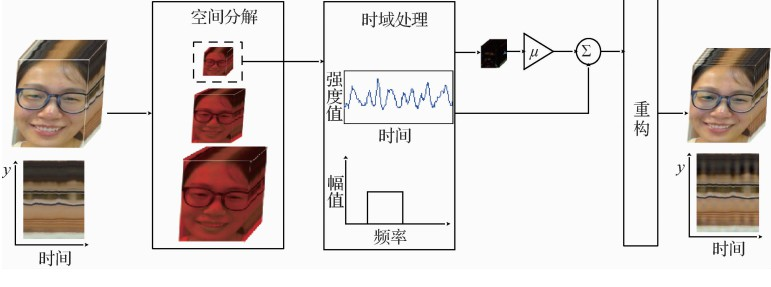
\includegraphics[width=4.5in]{example/BVP1.jpg}
\caption{视频图像序列颜色放大过程示意图}
\label{fig1:4-1}
\end{figure}

由于血液对绿光的吸收能力较强,因此绿色光的变化更能真实反映血容量的变化,而在YIQ空间中,绿色信息包含在Q通道内,因此,作者对预处理后的视频序列计算每幅图像Q通道的像素均值。

经过视频颜色放大算法后得到的BVP信号,仅是增加了幅值而并没有改变信号的频率特性,且每个信号都设置相同的放大因子,因此放大过程并不会影响BVP信号对HR,LF,HF等特征的提取。

\subsubsection{方法3 - ICA}

\begin{figure}[!htp]
\centering
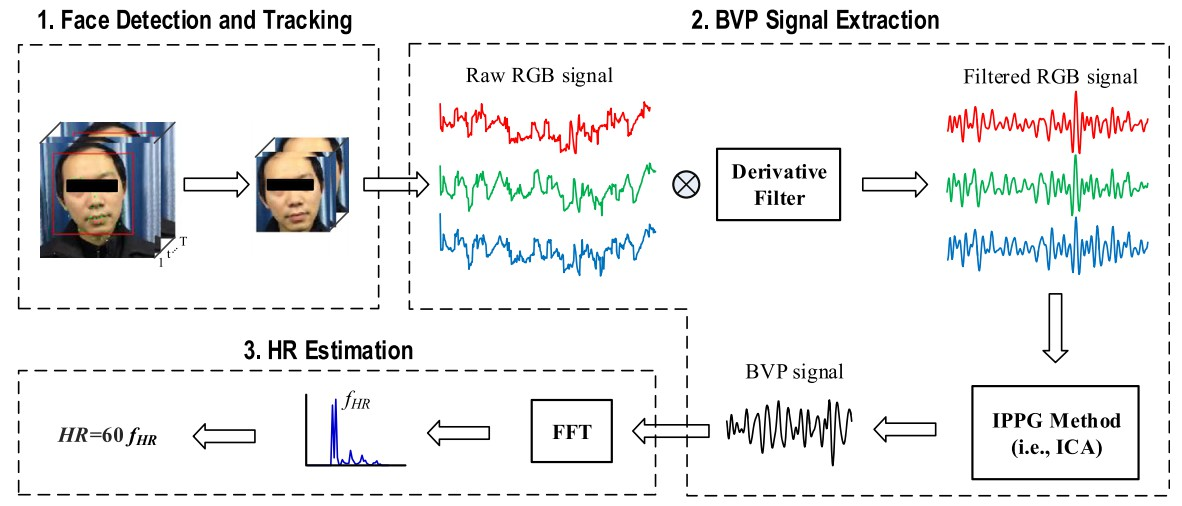
\includegraphics[width=5.5in]{example/BVP2.jpg}
\caption{心率估计流程图}
\label{fig1:4-1}
\end{figure}


\subsection{BVP信号特征提取}

在2018年《\href{https://xueshu.baidu.com/usercenter/paper/show?paperid=b22a6ba0c40126662ef983f6c530096d&site=xueshu_se&hitarticle=1}{融合表情和BVP生理信号的双模态视频情感识别}》一文中,作者对BVP生理信号提取多个特征,包括时域和频域等。

令$Z$代表着一个BVP信号$Z=[z_1,z_2,z_3,...,z_N]$,N代表视频帧的长度,首先在时间序列上对该信号提取下列能够反映BVP信号变化规律的统计学特征,用来表征血管的收缩情况,提供有关交感神经的活动信息,包括均值、标准差、一阶差分信号的绝对值均值、二阶差分信号的绝对值均值,以及归一化差分信号的绝对值均值。具体计算公式为
\begin{align}
& \mu_z = \frac{1}{N} \sum_{i=1}^N z_i \\
& \sigma_z = \sqrt{\frac{1}{N} \sum_{i = 1}^N(z_i - \mu_z)^2} \\
& \delta_z = \frac{1}{N - 1} \sum_{i = 1}^{N - 1}|z_{i+1} - z_i| \\
& \zeta_z = \frac{\sigma_z}{\delta_z} \\
& \gamma_z = \frac{1}{N-2} \sum_{i=1}^{N-2} |z_{i+2} - z_i| \\
& \xi_z = \frac{\gamma_z}{\delta_z}
\end{align}

为了获得BVP信号的子带频谱,将原信号进行傅里叶变换,把0 $\sim$ 4Hz等分成5个不重叠的子带,计算每个子带的能量均值和频谱熵,并求取在0.8 $\sim$ 2Hz范围内功率谱的最大幅值对应的频率$F_0$,频谱熵的计算公式为
\begin{align}
H_{sub} = \sum_{i = 1}^N f_i \cdot \log_2(f_i)
\end{align}

式中,$f_i$是频谱的第i个频率分量的能量$F_i$,的归一化,具体公式为
\begin{align}
f_i = \frac{F_i}{\sum_{i=1}^N F_i}; \quad i=1,...,N
\end{align}

再把5个子频带分成两份,前两个子带频谱看成是低频带LF,后3个看成是高频带HF,分别求取低频和高频的能量比值和熵比值。

作者通过计算BVP信号连续峰值之间的差值,得到心率变化(HRV),并将HRV 在时间序列上构成的信号称为G信号。类似于BVP信号,对G信号分别求取均值、标准差等统计学特征。记录G信号相邻点之间的差值大于50ms 的个数,
并求取它与BVP信号总的峰值个数的比值,并将其作为疲劳估计的生理信号特征之一。

\section{声纹识别}

\section{近5年来疲劳检测研究进展}

\cite{malov2019fatigue}

在2017年《\href{}{Fatigue Detection Techniques: A Review}》一文中,作者指出,呼吸率和心率是最明显的疲劳特征。在2017年《\href{https://ieeexplore.ieee.org/abstract/document/8258154/}{Sleep-deprived Fatigue Pattern Analysis using Large-Scale Selfies from Social Media}》一文中,作者通过使用高分辨率的人脸照片来确定人的疲劳程度。他们指出,对8个与疲劳高度相关的因素进行线性回归计算就足够了: 沉重的眼睑,发红的眼睛,黑眼圈,苍白的皮肤,下翻的嘴,浮肿的眼睛,呆滞的眼睛,眼睛周围的皱纹,皮肤缺陷或湿疹,以及嘴唇紧张。作者使用Face++ API 进行人脸对齐,并基于关键点提取感兴趣区域,然后使用VGG16从获得的区域中提取特征。作者指出,左眼和右眼,以及左眼和右眼的眼睑是分别作为独立感兴趣区域进行研究的。

在2019年《\href{https://xueshu.baidu.com/usercenter/paper/show?paperid=10050gc0dx5n0ex09m660eg0dr674514&site=xueshu_se&hitarticle=1}{A Realistic Dataset and Baseline Temporal Model for Early Drowsiness Detection}》一文中,作者将眼睛作为感兴趣区域,并为每只眼睛设置6个关键点用来疲劳检测,通过跟踪眨眼动作来检测疲劳。在本研究中,作者使用了一些现有的计算眨眼频率的方法,值得注意的是,这些方法的共同缺点是对频繁眨眼的人敏感性较低,因此作者将几种眨眼行为视为一个整体,并考虑如何适应不同的光照变化,适度的头部旋转和面部表情的变化。作者以10 分钟的视频作为源数据,处理完这段视频后,可以获得一个事件向量,其中每个事件都包含对应的数据:持续时间、振幅、速度和睁眼率。这里使用的模型是HM-LSTM网络,该方法的疲劳检测精度为65.2$\%$。


在2018年《\href{https://xueshu.baidu.com/usercenter/paper/show?paperid=1f7k0g20h77e0gh0wg5802d0cp212255&site=xueshu_se}{An
Intelligent Safety System for Human-Centered Semi-Autonomous Vehicles}》一文中,作者从概念上定义了一个用于汽车驾驶的安全系统原型。它由三个独立的注意模块组成:

1. 车道安全巡航模块:该模块主要工作是对道路进行标记,可以通过神经网络来定义适合汽车巡航的区域。

2. 驾驶员状态模块:确保对驾驶员面部进行记录,检测驾驶员头部姿势、眨眼和闭眼。并且还要对驾驶室进行记录,以评估司机的姿势,了解他的头、身体和手臂的位置。

3. 车辆交互模块:作者通过使用特定的设备连接到车辆系统,并从控制单元和外部传感器以及摄像机获取数据。

在2018年《\href{https://xueshu.baidu.com/usercenter/paper/show?paperid=67fb1a113a128dd8d5e40fec74fccf4b&site=xueshu_se&hitarticle=1}{Real-time Driver Drowsiness Detection for Android Application Using Deep Neural Networks Techniques}》一文中,作者使用Dlib库对视频帧中司机脸上的68个关键点进行定位,这些关键点被归一化后输入到神经网络中。驾驶员在不戴眼镜的实验中达到了87.1$\%$的准确度,而在戴墨镜的实验中最小准确率可达到了75.1$\%$,而平均检测准确率为80.9$\%$。


%%# -*- coding: utf-8-unix -*-
%%==================================================
chap5\chapter{疲劳检测相关专业术语}

\section{信号处理知识}

\subsection{共振峰}

\subsection{倒谱}

参考\href{https://baike.baidu.com/item/%E5%80%92%E8%B0%B1/9851556?fr=aladdin}{百度百科:倒谱}

倒谱(cepstrum)一种信号的傅里叶变换谱经对数运算后再进行的傅里叶反变换。由于一般傅里叶谱是复数谱,因而又称复倒谱。


\section{医学知识}

\subsection{交感神经和副交感神经}
LF,HF,LF/HF均衡性

\subsection{纺锤波}
EGG不同信号频段的纺锤波

\subsection{运动伪影}

除BPF和ASF外,最小均方(LMS)的自适应滤波器还能有效地减少在BVP信号\cite{liu2018self}中的运动伪影,LMS滤波器的一个局限性是它对输入信号的缩放很敏感。

运动伪影是磁共振成像最大的问题之一 ,在许多磁共振检查中运动伪影不可避免的随机噪声更明显地降低图像质量 ,它使图像模糊并且沿相位编码方向产生鬼影运动包括各种生理运动和身体运动。\footnote{\url{https://zhidao.baidu.com/question/1545558467918962427.html}}
伪影(Artifacts):是由于设备或病人造成的。
是指原本被扫描物体并不存在而在图像上却出现的各种形态的影像。伪影大致分为与患者有关和与机器有关的两类。
CT图像伪影指图像上与实际解剖结构不相符的密度异常变化,它涉及CT机部件故障、校准不够及算法误差甚至错误等项目,要消除此类伪影,需根据图像伪影的形状、密度变化值及扫描参数等进行具体问题具体分析。第三代CT机的图像伪影具有一定的普遍性,又特别以环状伪影为最常见。
分类有:
\begin{itemize}
    \item 运动伪影
    \item 混淆伪影或包裹伪影
    \item 化学移位伪影
    \item 化学性配准不良伪影
    \item 截断伪影
    \item 磁敏感伪影
    \item 拉链伪影
    \item 交叉激励
\end{itemize}

MR图像的运动伪影通常是指由于受检者的宏观运动引起的伪影。这些运动可以是自主运动如肢体运动,吞咽等,也可以是非自主运动如心跳,血管搏动等。运动可以是随机的如胃肠蠕动,吞咽等,也可以是周期性运动如心跳和血管搏动等
\footnote{MR运动伪影 \quad \url{http://www.360doc.com/content/15/1207/09/15645340_518464634.shtml}}。

运动伪影出现的原因主要是由于在MR信号采集过程中,运动器官在每一次激发,编码及信号采集时所处的位置或形态发生了变化,因此将出现相位的偏移,在傅里叶转换时会把这种相位的偏移误当成相位编码方向的位置信息,把组织的信号配置到一个错误的位置上,从而出现运动伪影。

运动伪影具有以下特点:
\begin{itemize}
    \item 主要出现在相位编码方向上;
    \item 伪影的强度取决于运动结构的信号强度,后者信号强度越高,相应的伪影越明显;
    \item 伪影复制的数目,位置受基本正弦运动的相对强度,TR,NEX,FOV等因素的影响。
\end{itemize}

随机自主运动伪影是指在不具有周期性且受检者能够自主控制的运动造成的伪影,如吞咽,眼球转动,肢体运动等造成的伪影。随机自主运动伪影的特点:
\begin{itemize}
    \item 主要造成图像迷糊;
    \item 伪影出现在相位编码方向;
    \item 受检者可以控制。
\end{itemize}

\begin{figure}[t]
\centering
    
\includegraphics[width=5in]{example/test.pdf}
    \caption{EEG信号.}
\end{figure}

\subsection{公式排版}

这里有举一个长公式排版的例子,来自\href{http://www.tex.ac.uk/tex-archive/info/math/voss/mathmode/Mathmode.pdf}{《Math mode》}:

\begin {multline}
\frac {1}{2}\Delta (f_{ij}f^{ij})=
2\left (\sum _{i<j}\chi _{ij}(\sigma _{i}-
\sigma _{j}) ^{2}+ f^{ij}\nabla _{j}\nabla _{i}(\Delta f)+\right .\\
\left .+\nabla _{k}f_{ij}\nabla ^{k}f^{ij}+
f^{ij}f^{k}\left [2\nabla _{i}R_{jk}-
\nabla _{k}R_{ij}\right ]\vphantom {\sum _{i<j}}\right )
\end{multline}

\subsection{SI单位}

使用\verb+siunitx+宏包可以方便地输入SI单位制单位,例如\verb+\SI{5}{\um}+可以得到\SI{5}{\um}。

\subsection{定理环境}

在这个模板中,定义了如下几个环境
remark(注),mythm(定理),myprop(性质),mydef(定义),example(例)。
amsmath还提供了一个proof(证明)的环境。
我们举例说明它们的用法。

注环境
\begin{remark}
	存在事先给定的一系列基本操作,并且这些基本操作永远不会改变。
\end{remark}
\begin{remark}
	每个操作都可逆。
	\label{o1.2}
\end{remark}
\begin{remark}
	每一个操作都是确定性的。
\end{remark}
\begin{remark}
	各个操作可以按任何顺序组合。
\end{remark}

性质环境
\begin{myprop}{}{}
	存在一些预先定义的永不发生改变的作用(action)。
\end{myprop}

\begin{myprop}{}{}
	每一个作用都可逆。
\end{myprop}

\begin{myprop}{}{}
	每个作用都是确定性的。
\end{myprop}

\begin{myprop}{}{}
	任意的一系列连续的作用仍然是一个作用。
\end{myprop}

例子环境
\begin{example}
	天地玄黄,宇宙洪荒。
	\soln
	
	日月盈仄,辰宿列张。
\end{example}

定义环境
\begin{mydef}{域}{1}
	设$S$为一个非空集合,其上有“加法”(记作$+$)与“乘法”(记作$\cdot$)两种代数运算. 若满足以下条件,则称$(S,+,\cdot)$ 构成一个域(field).
	\begin{itemize}
		\item[(1)] $(S,+)$构成一个交换群.
		\item[(2)] 若记$S^{*}=S-\{0\}$,其中$0$为群$(S,+)$中的单位元,则$(S^{*},\cdot)$也构成一个交换群.
		\item[(3)] 乘法对加法有分配律:$a ( b + c ) = a b + a c$.
	\end{itemize}
\end{mydef}

关键点环境
\begin{keypoint}
	伽罗瓦理论在分析从有理数域$\mathbb{ Q }$扩张到新的域的运算或操作时很有用。我们的大问题可以用伽罗瓦理论来回答,数学中其他的一些历史问题也同样可以用伽罗瓦理论来解答。
\end{keypoint}

定理环境
\begin{mythm}{望远镜公式}{2}
	$\left[\mathbb{Q}(a, b) : \mathbb{Q}\right]=\left[\mathbb{Q}(a, b) : \mathbb{Q}(a)\right]\left[\mathbb{Q}(a) : \mathbb{Q}\right] $
\end{mythm}

\begin{proof}
	
	\rthm{thm:2}告诉我们,对任意$s\in S$,均有$\lvert Orb(s)\rvert \cdot \lvert Stab(s)\rvert=\lvert G\rvert=p$. 于是$\lvert Orb(s)\rvert $ 整除$p$,这里$p$是一个素数。从而$\lvert Orb(s)\rvert $等于1或$p$,也就是说,\textbf{所有轨道的大小要么为1,要么为$p$}. 于是整个集合$S$就被划分为两部分,一部分是大小为1 的轨道,另一部分是大小为$p$的轨道,如图9.4所示。
	
	假设大小为1的轨道有$m$个,大小为$p$的轨道有$n$个,则有
 \begin{equation}
		m+p\cdot n=\lvert S\rvert
 \end{equation}
	注意到\rdef{def:1},\textbf{那些$\lvert Orb(s)\rvert =1$的元素$s$即为稳定元},这就表明有$m$个稳定元。从上式立刻看出$\lvert S \rvert \equiv  m\; (\bmod\; p)$.	
\end{proof}

\section{表格}

这一节给出的是一些表格的例子,如表\ref{tab1}所示。

\begin{table}[!hpb]
	\centering
	\bicaption[指向一个表格的表目录索引]
	{一个颇为标准的三线表格\footnotemark[1]}
	{A Table}
	\label{tab1}
	\begin{tabular}{@{}llr@{}} \toprule
		\multicolumn{2}{c}{Item} \\ \cmidrule(r){1-2}
		Animal & Description & Price (\$)\\ \midrule
		Gnat & per gram & 13.65 \\
		& each & 0.01 \\
		Gnu & stuffed & 92.50 \\
		Emu & stuffed & 33.33 \\
		Armadillo & frozen & 8.99 \\ \bottomrule
	\end{tabular}
\end{table}
\footnotetext[1]{这个例子来自\href{http://www.ctan.org/tex-archive/macros/latex/contrib/booktabs/booktabs.pdf}{《Publication quality tables in LATEX》}(booktabs 宏包的文档)。这也是一个在表格中使用脚注的例子,请留意与threeparttable实现的效果有何不同。}

下面一个是一个更复杂的表格,用threeparttable实现带有脚注的表格,如表\ref{tab2}。

\begin{table}[!htpb]
	\bicaption[出现在表目录的标题]
	{一个带有脚注的表格的例子}
	{A Table with footnotes}
	\label{tab2}
	\centering
	\begin{threeparttable}[b]
		\begin{tabular}{ccd{4}cccc}
			\toprule
			\multirow{2}{6mm}{total}&\multicolumn{2}{c}{20\tnote{1}} & \multicolumn{2}{c}{40} &  \multicolumn{2}{c}{60}\\
			\cmidrule(lr){2-3}\cmidrule(lr){4-5}\cmidrule(lr){6-7}
			&www & \multicolumn{1}{c}{k} & www & k & www & k \\ % 使用说明符 d 的列会自动进入数学模式,使用 \multicolumn 对文字表头做特殊处理
			\midrule
			&$\underset{(2.12)}{4.22}$ & 120.0140\tnote{2} & 333.15 & 0.0411 & 444.99 & 0.1387 \\
			&168.6123 & 10.86 & 255.37 & 0.0353 & 376.14 & 0.1058 \\
			&6.761    & 0.007 & 235.37 & 0.0267 & 348.66 & 0.1010 \\
			\bottomrule
		\end{tabular}
		\begin{tablenotes}
			\item [1] the first note.% or \item [a]
			\item [2] the second note.% or \item [b]
		\end{tablenotes}
	\end{threeparttable}
\end{table}

\section{插入图片}

\XeTeX 可以很方便地插入PDF、PNG、JPG格式的图片。插入PNG/JPG的例子如\ref{fig1}所示。
这两个水平并列放置的图共享一个“图标题”(table caption),没有各自的小标题。

\begin{figure}[!htp]
\centering

\includegraphics[width=4cm]{example/by-nc.png}
\hspace{1cm}
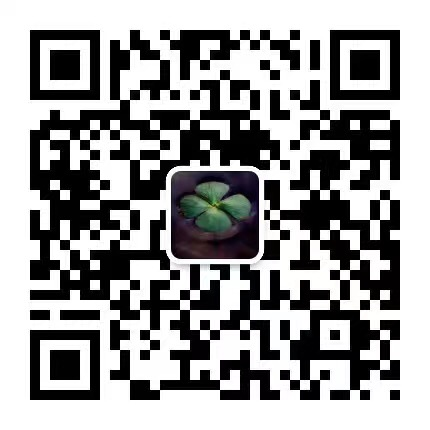
\includegraphics[width=4cm]{example/gzh.jpg}
\bicaption{中文题图}
{English caption}
\label{fig1}
\end{figure}

这里还有插入EPS图像和PDF图像的例子,如图\ref{fig2}和图\ref{fig3}。这里将EPS和PDF图片作为子图插入,每个子图有自己的小标题。子图标题使用subcaption宏包添加。

\begin{figure}[!htp]
\centering
\subcaptionbox{EPS 图像\label{fig2}}[3cm] %标题的长度,超过则会换行,如下一个小图。
{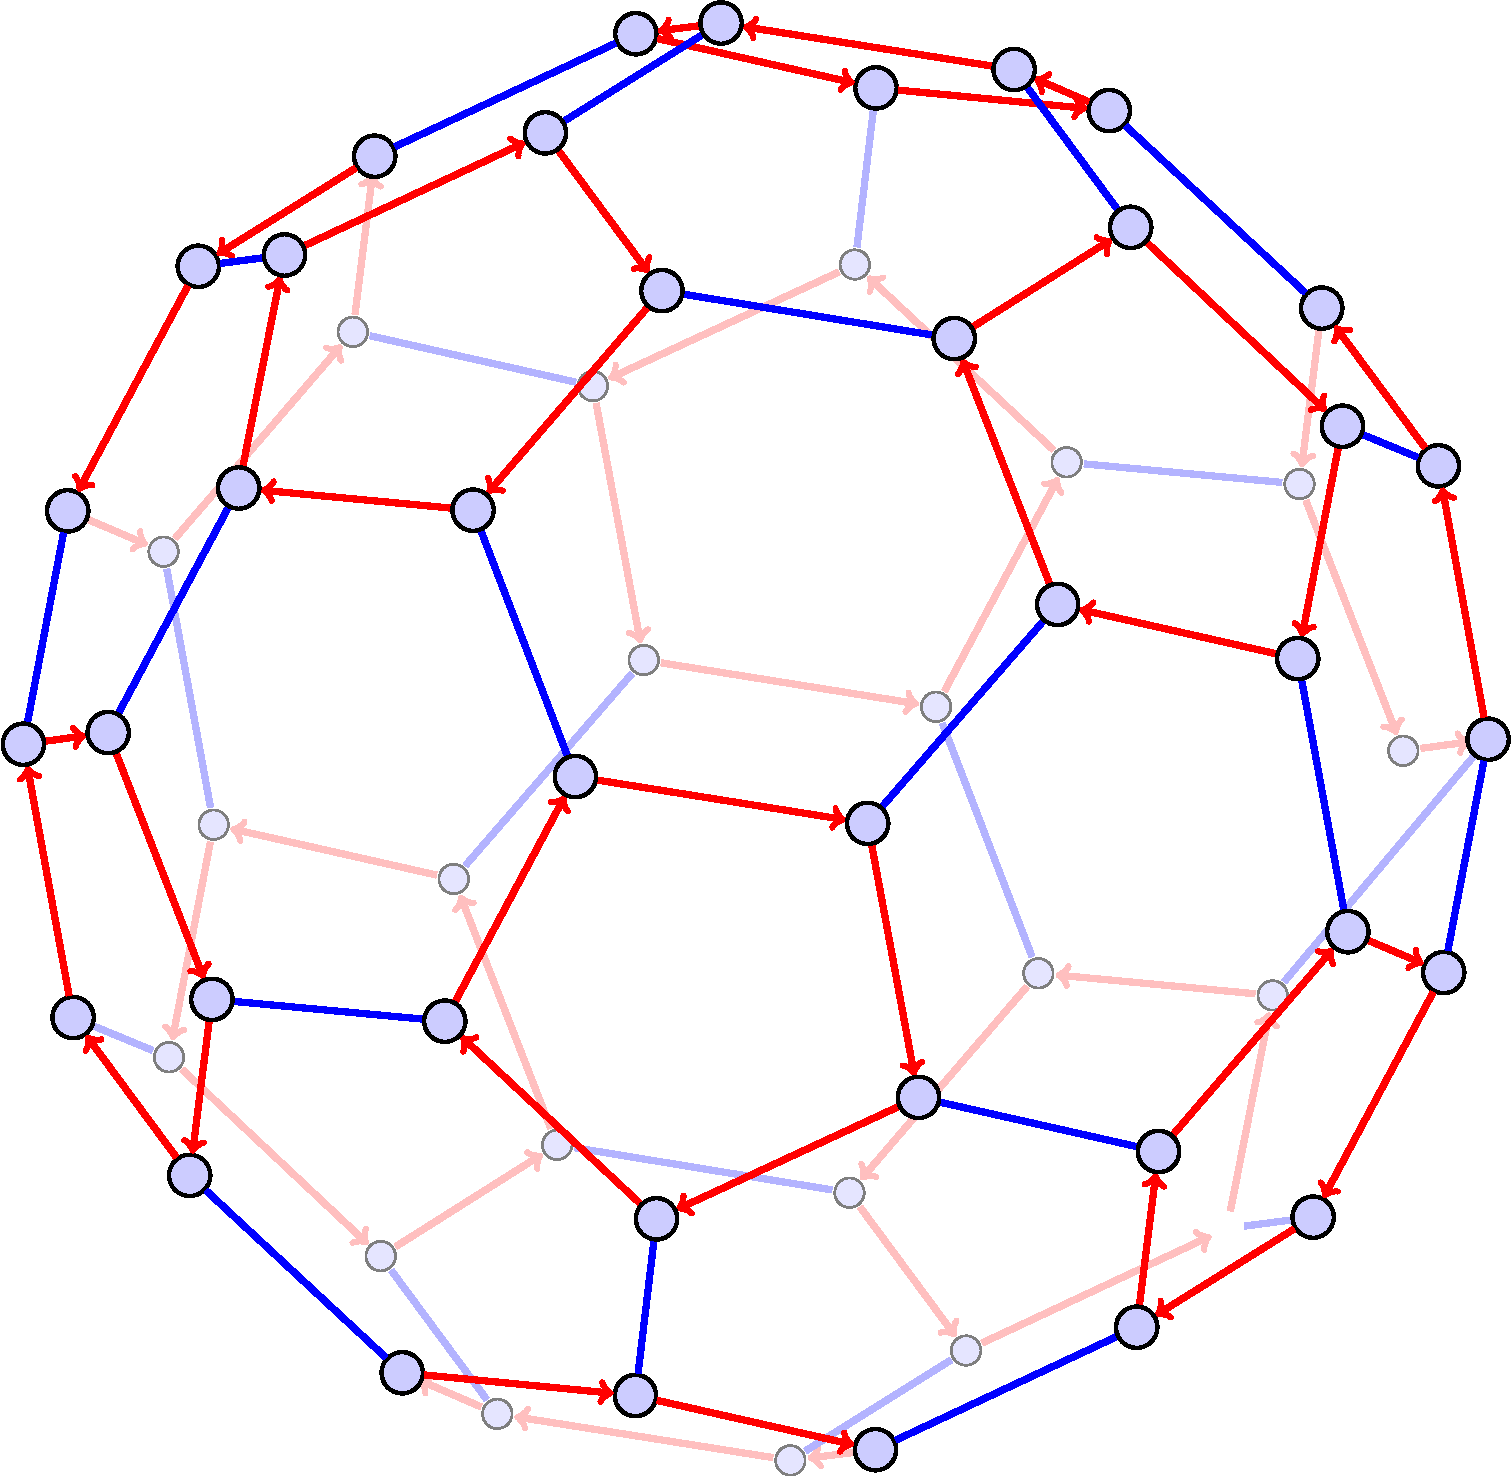
\includegraphics[height=2.5cm]{example/m2.pdf}}
\hspace{4em}
\subcaptionbox{PDF 图像,注意这个图略矮些。如果标题很长的话,它会自动换行\label{fig3}}
{	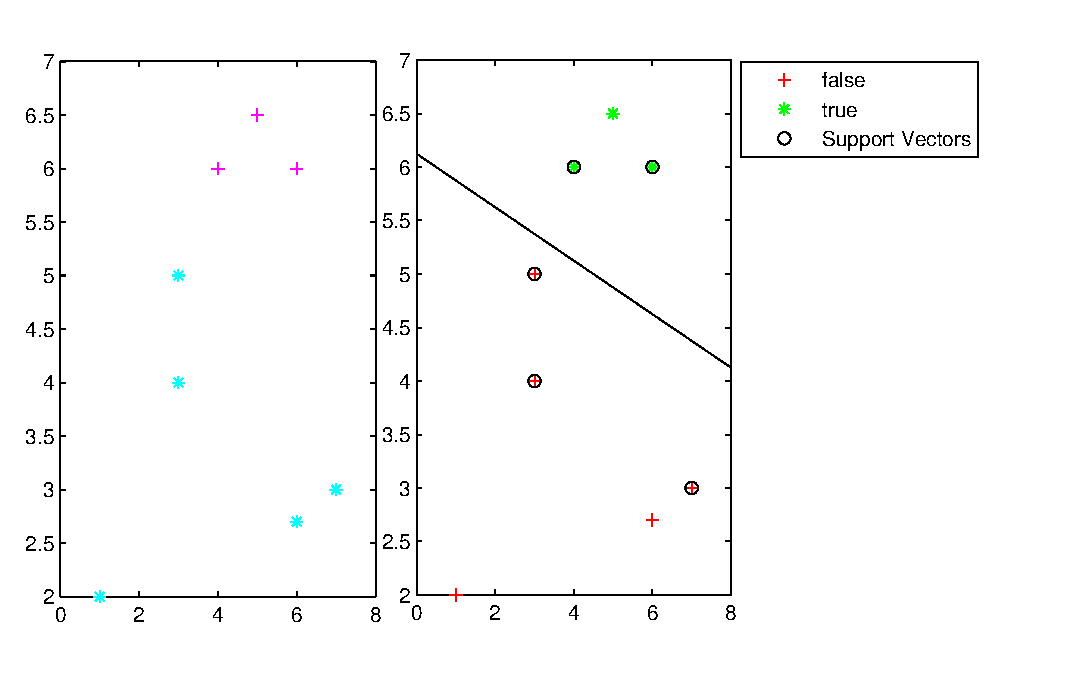
\includegraphics[scale=0.5]{example/figep.eps}}
\bicaption{插入eps和pdf的例子(使用 subcaptionbox 方式)}{An EPS and PDF demo with subcaptionbox}
\label{fig4}
\end{figure}




\section{插入代码}

这里给一个使用listings宏包插入源代码的例子:
\begin{lstlisting}[language={C}, caption={一段C源代码}]
#include <stdio.h>
#include <unistd.h>
#include <sys/types.h>
#include <sys/wait.h>

int main() {
pid_t pid;

switch ((pid = fork())) {
case -1:
printf("fork failed\n");
break;
case 0:
/* child calls exec */
execl("/bin/ls", "ls", "-l", (char*)0);
printf("execl failed\n");
break;
default:
/* parent uses wait to suspend execution until child finishes */
wait((int*)0);
printf("is completed\n");
break;
}

return 0;
}
\end{lstlisting}


\section{参考文献管理}
\label{sec2.5}
\LaTeX 具有将参考文献内容和表现形式分开管理的能力,涉及三个要素:参考文献数据库、参考文献引用格式、在正文中引用参考文献。
这样的流程需要多次编译:
\begin{enumerate}[noitemsep,topsep=0pt,parsep=0pt,partopsep=0pt]
\item 用户将论文中需要引用的参考文献条目,录入纯文本数据库文件(bib文件)。
\item 调用xelatex对论文模板做第一次编译,扫描文中引用的参考文献,生成参考文献入口文件(aux)文件。
\item 调用bibtex,以参考文献格式和入口文件为输入,生成格式化以后的参考文献条目文件(bib)。
\item 再次调用xelatex编译模板,将格式化以后的参考文献条目插入正文。
\end{enumerate}

参考文献数据库(thesis.bib)的条目,可以从Google Scholar搜索引擎\footnote{\url{https://scholar.google.com}}、CiteSeerX搜索引擎\footnote{\url{http://citeseerx.ist.psu.edu}}中查找,文献管理软件Papers\footnote{\url{http://papersapp.com}}、Mendeley\footnote{\url{http://www.mendeley.com}}、JabRef\footnote{\url{http://jabref.sourceforge.net}} 也能够输出条目信息。

下面是在Google Scholar上搜索到的一条文献信息,格式是纯文本:

\begin{lstlisting}[caption={从Google Scholar找到的参考文献条目}, label=googlescholar, escapeinside="", numbers=none]
@phdthesis{"白2008信用风险传染模型和信用衍生品的定价",
title={"信用风险传染模型和信用衍生品的定价"},
author={"白云芬"},
year={2008},
school={"上海交通大学"}
}
\end{lstlisting}

推荐修改后在bib文件中的内容为:

\begin{lstlisting}[caption={修改后的参考文献条目}, label=itemok, escapeinside="", numbers=none]
@phdthesis{bai2008,
title={"信用风险传染模型和信用衍生品的定价"},
author={"白云芬"},
date={2008},
address={"上海"},
school={"上海交通大学"}
}
\end{lstlisting}

参考文献的引用:
\begin{itemize}
\item 参考文献在正文中被引用,使用命令\verb+\cite{key}+,如\cite{M91}。
\item 参考文献未引用但仍希望列在书末的参考文献中,使用命令\verb+\nocite{key}+,如\verb+\nocite{WI64,G03,D01,JS03}+.
\end{itemize}
\nocite{WI64,G03,D01,JS03}

%\chapter{充满正能量和充满负能量的人 - 个人篇}

在我看来,正能量是一种短暂性忘却顾虑,它总是抱着某种希望,能够推动人向前的一种“积极“力量,而负能量是一种不断放大风险顾虑,并对其进行思考和分析的“平淡理性“能量。对于正能量和负能量的使用熟练程度因人而异。

不喜欢用正能量,负能量来区分人。因为人的情感包括喜怒哀乐等,十分复杂,并不能完全明确的将其划分成正负两类。那些自以为正能量满满的人,往往是自以为是的; 而负能量的人中往往也有很多是明辨是非的。这两类人并没有严格的好坏区分。正能量可能会做错事,负能量可能会做对事。

正能量的人,他内心往往也隐藏着负能量,负能量的人也向往着拥有正能量。但是对于这两种能量,过尤而不及。对于真正想要成长来说,适当的负能量是必要的土壤; 而适当的正能量是你撒下的种子,它会引导你去克服困难,迎难而上。

这两股能量此消彼长,比如当你消耗着自己的正能量无私帮助他人时,你的负能量也会随之增加(这就是能量守恒)。有些人正能量能够极速增加到一定的水平,但是储存不了多久,消耗得特别快,而转化成的负能量可以储存比较长时间,消耗很慢。

因此如何将两种能量保持在平稳但有一定波动水平上至关重要,有网友建议画画,而我个人感觉冥想是个不错的办法,但是要坚持做下去。因为正能量在被消耗的过程中,会转化成现实中的创造力活动,消耗正能量产生的负能量却被储存起来,不能被消耗,这时就可以通过冥想来让这种能量以蒸发的方式慢慢消散(冥想的时间自己去定义)

%\include{tex/chapter7}
%


%\include{tex/chapter9}
%\include{tex/chapter10}
\backmatter	
%======================================================================
% 打印参考文献
1111111\cite{123a}
\printbibliography[heading=bibintoc]
\makeatletter
\makeatother
\end{document}
